\documentclass[conf,hidelinks]{new-aiaa} % insert '[draft]' option to show overfull boxes
%---------- USER-ADDED PACKAGES
\usepackage{amsmath}
\usepackage[english]{babel}
\usepackage{booktabs} 	% For tables
\usepackage{breqn}
\usepackage{caption} 	% For subfigures
\usepackage[capitalise]{cleveref}
\usepackage{subfigure}
\usepackage{float}
\usepackage[T1]{fontenc}
\usepackage{gensymb}
\usepackage{graphicx}
\usepackage{import}		% Package for breaking down lengthy documents into submodules
\usepackage{pdfpages} 	% To include PDF pages in appendix
\usepackage{placeins}	% Floatbarrier
\usepackage{siunitx} 	% For the degree symbol "\ang{}"
\usepackage{titlesec}
\usepackage{todonotes}
\usepackage{type1cm}
\usepackage{wasysym}
\usepackage{wrapfig}	% For inline figures
\usepackage{listings} %--- For including MATLAB code ---%
\usepackage{color} %red, green, blue, yellow, cyan, magenta, black, white
\definecolor{mygreen}{RGB}{28,172,0} % color values Red, Green, Blue
\definecolor{mylilas}{RGB}{170,55,241}
\lstset{language=Matlab,%
	basicstyle=\footnotesize\ttfamily,
	breaklines=true,%
	morekeywords={matlab2tikz},
	keywordstyle=\color{blue},%
	morekeywords=[2]{1}, keywordstyle=[2]{\color{black}},
	identifierstyle=\color{black},%
	stringstyle=\color{mylilas},
	commentstyle=\color{mygreen},%
	showstringspaces=false,%without this there will be a symbol in the places where there is a space
	numbers=left,%
	numberstyle={\tiny \color{black}},% size of the numbers
	numbersep=9pt, % this defines how far the numbers are from the text
	emph=[1]{for,end,break},emphstyle=[1]\color{red}, %some words to emphasise
}
%---End MATLAB code inclusion package ---%
\makeatletter
\makeatother
% Variables
\newcommand{\figwidth}{3.4in}				% Width of single figure
\newcommand{\figheight}{2.43in}				% Height of single figure
\newcommand{\figwidthlegend}{4.0in}			% Width of single figure with outer legend
\newcommand{\doubfigf}{.475}				% Text width factor in double figure
\AtBeginDocument{\renewcommand{\abstractname}{}}

%\title{Best Practices for Wake Model and Optimization Algorithm Selection in Wind Farm Layout Optimization}

%\author{Nicholas F. Baker\footnote{Masters Student, Department of Mechanical Engineering, 360 EB, Provo, UT 84602, AIAA Student Member},
%		 Andrew P. J. Stanley\footnote{Ph.D. Candidate, Department of Mechanical Engineering, 360 EB, Provo, UT 84602, AIAA Student Member},
%		 Jared J. Thomas\footnote{Ph.D. Student, Department of Mechanical Engineering, 360 EB, Provo, UT 84602, AIAA Student Member},
%		 and Andrew Ning\footnote{Assistant Professor, Department of Mechanical Engineering, 360 EB, Provo, UT 84602, AIAA Senior Member}}
%	\affil{Brigham Young University, Provo, Utah 84602.}
%\author{Katherine Dykes\footnote{Senior Engineer, National Wind Technology Center, 15013 Denver West Pkwy, Golden, CO 80401}}
%	\affil{National Renewable Energy Laboratory, Golden, Colorado 80401}

\begin{document}
%\maketitle{}

%---------- Tables ----------%

\begin{table}[h!]
    \begin{center}
        \caption{16 turbine scenario participant results}
        \label{tab:results1}
        \begin{tabular}{r l l c r r}
            \hline
            Rank	& Algorithm											& sub\#	& Grad.	& AEP			& Increase		\\	%& Norm.		\\
            \hline
            1       & Quantum								            & 12    & GF	& 421561.8972	&	14.88 \% 	\\ %&	- \% 	\\
            2       & SNOPT\texttt{+}WEC								& 4     & G		& 418924.4064	&	14.17 \% 	\\ %&	- \% 	\\
            3       & fmincon											& 5     & G		& 414141.2938	&	12.86 \% 	\\ %&	-1.14 \% 	\\
            4       & SNOPT												& 8     & G		& 412251.1945	&	12.35 \% 	\\ %&	-1.59 \% 	\\
			5       & SNOPT												& 1     & G		& 411182.2200	&	12.06 \% 	\\ %&	-1.85 \% 	\\
			6		& SLSQP												& 11	& G		& 409850.3275	&	11.69 \% 	\\ %&	-3.85 \% 	\\
            7       & Preconditioned Sequential Quadratic Programming	& 2     & G		& 409689.4417	&	11.65 \% 	\\ %&	-2.20 \% 	\\
            8       & Multistart Interior-Point							& 10    & G		& 408360.7813	&	11.29 \% 	\\ %&	-2.52 \% 	\\
			9       & Full Pseudo-Gradient Approach						& 3     & GF	& 402318.7567	&	9.64 \% 	\\ %&	-3.96 \% 	\\
            10      & Basic Genetic Algorithm							& 7     & GF	& 392587.8580	&	6.99 \% 	\\ %&	-6.29 \% 	\\
            11      & Simple Particle Swarm Optimization				& 6     & GF	& 388758.3573	&	5.95 \% 	\\ %&	-7.20 \% 	\\
            12      & Simple Pseudo-Gradient Approach					& 9     & GF	& 388342.7004	&	5.83 \% 	\\ %&	-7.30 \% 	\\
            13		& (Example Layout)									& -		& -		& 366941.5712	&	- 			\\ %&	-12.41 \% 	\\
            \hline
        \end{tabular}
    \end{center}

    \begin{center}
        \caption{36 turbine scenario participant results}
        \label{tab:results2}
        \begin{tabular}{r l c c l r}
            \hline
            Rank	& Algorithm											& sub\#	& Grad.	& AEP			& Increase		\\	%& Norm.		\\
            \hline
            1       & Quantum								            & 12    & GF	& 882383.3040	&	19.58 \% 	\\ %&	- \% 	\\
            2		& SNOPT\texttt{+}WEC								& 4		& G		& 863676.2993   &	17.05 \% 	\\ %&	- \% 	\\
            3		& Multistart Interior-Point							& 10	& G		& 851631.9310	&	15.42 \% 	\\ %&	-1.39 \% 	\\
            4		& Preconditioned Sequential Quadratic Programming	& 2     & G		& 849369.7863	&	15.11 \% 	\\ %&	-1.66 \% 	\\
			5		& SNOPT												& 8     & G		& 846357.8142	&	14.70 \% 	\\ %&	-2.01 \% 	\\
			6		& SLSQP												& 11	& G		& 846255.1503	&	14.68 \% 	\\ %&	-3.85 \% 	\\
            7		& SNOPT												& 1     & G		& 844281.1609	&	14.42 \% 	\\ %&	-2.25 \% 	\\
            8		& Full Pseudo-Gradient Approach						& 3     & GF	& 828745.5992	&	12.31 \% 	\\ %&	-4.04 \% 	\\
            9		& fmincon											& 5     & G		& 820394.2402	&	11.18 \% 	\\ %&	-5.01 \% 	\\
            10		& Simple Pseudo-Gradient Approach					& 9     & GF	& 813544.2105	&	10.25 \% 	\\ %&	-5.80 \% 	\\
            11		& Basic Genetic Algorithm							& 7     & GF	& 777475.7827	&	5.37 \% 	\\ %&	-9.98 \% 	\\
            12		& Simple Particle Swarm Optimization				& 6     & GF	& 776000.1425	&	5.17 \% 	\\ %&	-14.56 \% 	\\
            13		& (Example Layout)									& -		& -		& 737883.0985	&	- 			\\ %&	-14.57 \% 	\\
            \hline
        \end{tabular}
    \end{center}

    \begin{center}
        \caption{64 turbine scenario participant results}
        \label{tab:results3}
        \begin{tabular}{r l c c l r}
            \hline
            Rank	& Algorithm											& sub\#	& Grad.	& AEP			& Increase		\\	%& Norm.		\\
            \hline
            1       & Quantum								            & 12    & GF	& 1526474.8025	&	17.88 \% 	\\ %&	- \% 	\\
            2		& SNOPT\texttt{+}WEC								& 4 	& G		& 1513311.1936	&	16.86 \% 	\\ %&	- \% 	\\
			3		& Preconditioned Sequential Quadratic Programming	& 2		& G		& 1506388.4151	&	16.33 \% 	\\ %&	-0.46 \% 	\\
			4		& SLSQP												& 11	& G		& 1484287.2607	&	14.62 \% 	\\ %&	-3.85 \% 	\\
            5		& Multistart Interior-Point							& 10	& G		& 1480850.9759	&	14.35 \% 	\\ %&	-2.15 \% 	\\
            6		& SNOPT												& 1		& G		& 1476689.6627 	&	14.03 \% 	\\ %&	-2.42 \% 	\\
			7		& Full Pseudo-Gradient Approach						& 3		& GF	& 1455075.6084	&	12.36 \% 	\\ %&	-3.85 \% 	\\
            8		& SNOPT												& 8		& G		& 1445967.3772	&	11.66 \% 	\\ %&	-4.45 \% 	\\
            9		& Simple Pseudo-Gradient Approach					& 9		& GF	& 1422268.7144	&	9.83 \% 	\\ %&	-6.02 \% 	\\
            10		& Simple Particle Swarm Optimization				& 6		& GF    & 1364943.0077	&	5.40 \% 	\\ %&	-9.80 \% 	\\
            11		& fmincon											& 5		& G		& 1336164.5498 	&	3.18 \% 	\\ %&	-11.71 \% 	\\
            12		& Basic Genetic Algorithm							& 7		& GF	& 1332883.4328	&	2.93 \% 	\\ %&	-11.92 \% 	\\
            13		& (Example Layout)									& -		& -		& 1294974.2977	&	- 			\\ %&	-14.43 \% 	\\
            \hline
        \end{tabular}
    \end{center}
\end{table}

%---------- Display of layouts ----------%
\newpage
\section*{Appendix}
This appendix contains plots of the optimized wind farm layouts submitted by all participants for case study 1. The optimized layouts for case study 1 are shown in \cref{fig:16turbs,fig:36turbs,fig:64turbs} for the 16, 36, and 64 turbine wind farms, respectively.

\begin{figure}[htbp!]
	\centering
	\subfigure[\textit{sub1}]{
		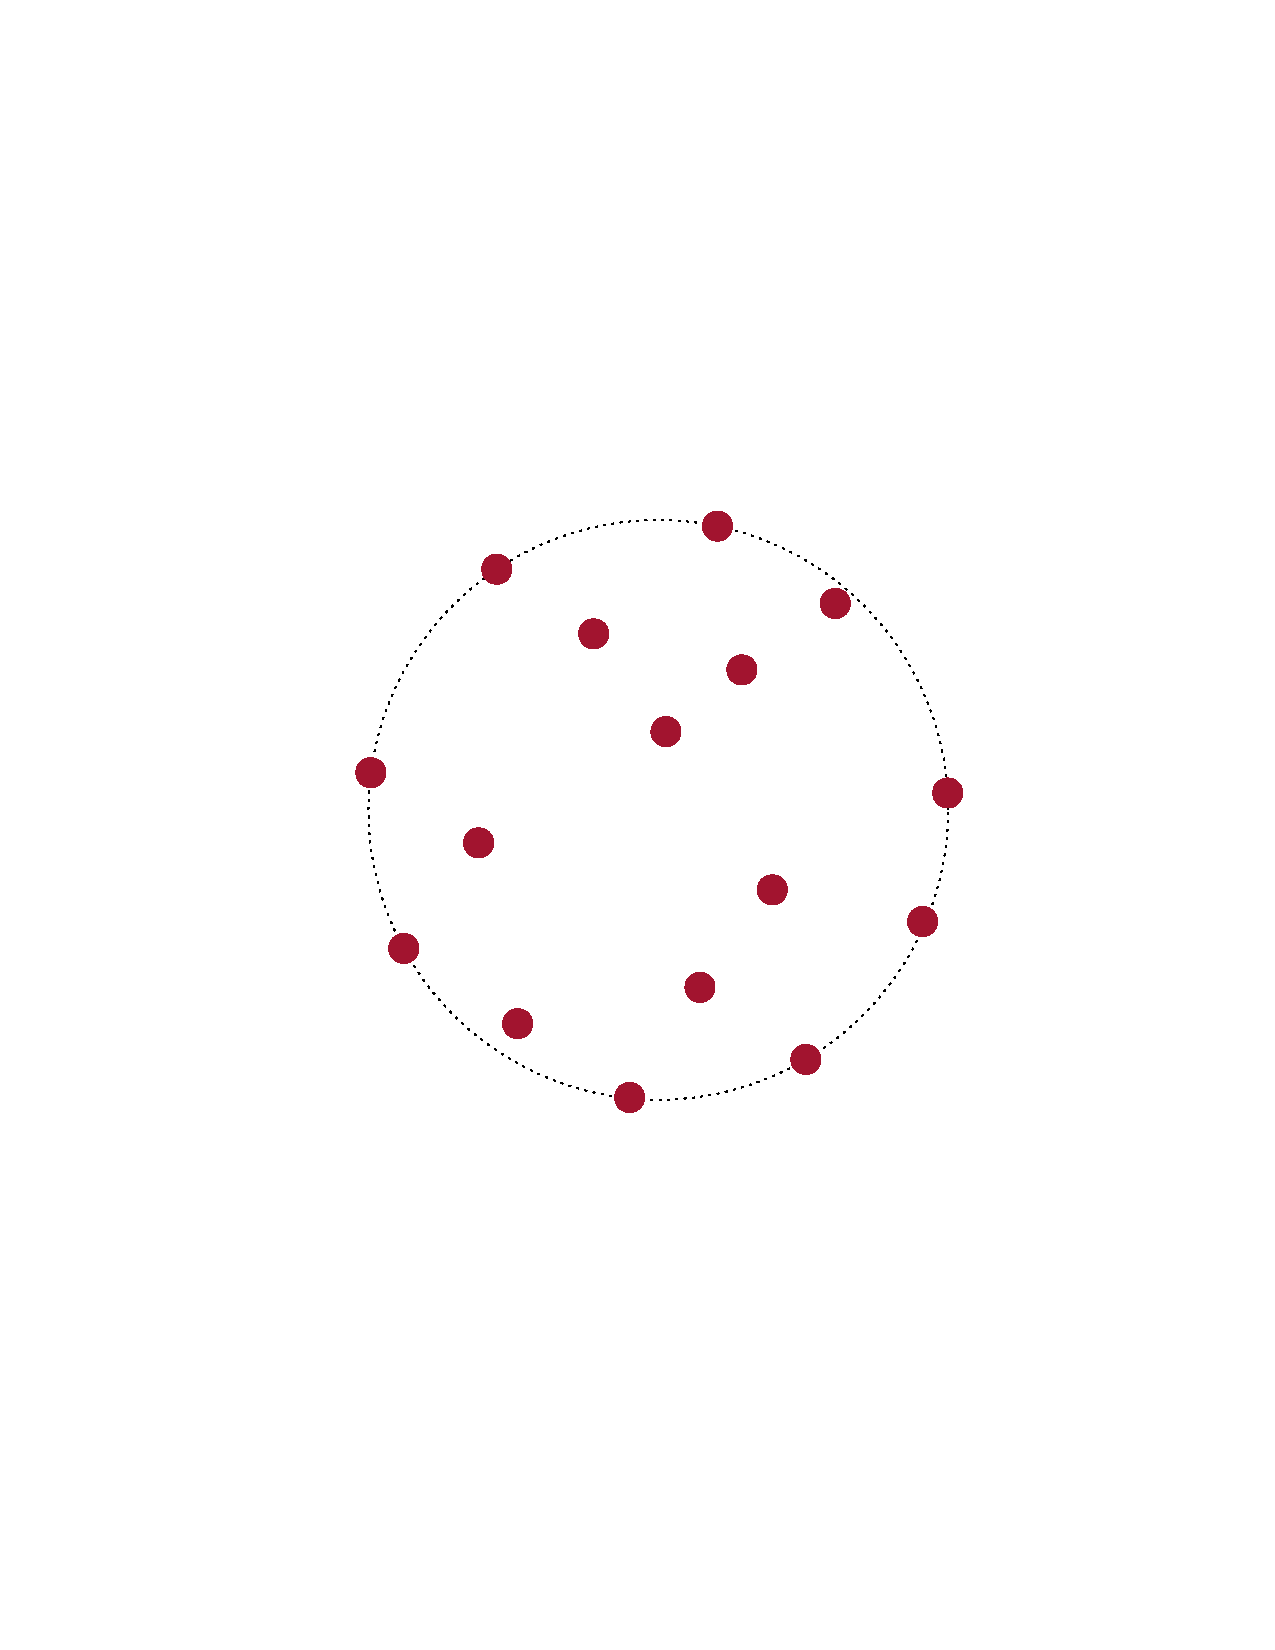
\includegraphics[clip, width=0.3\textwidth, scale=0.025, trim={3cm 8cm 3cm 8cm}]{figures/iea37-opt16-par1.pdf}
	}
	\subfigure[\textit{sub2}]{
		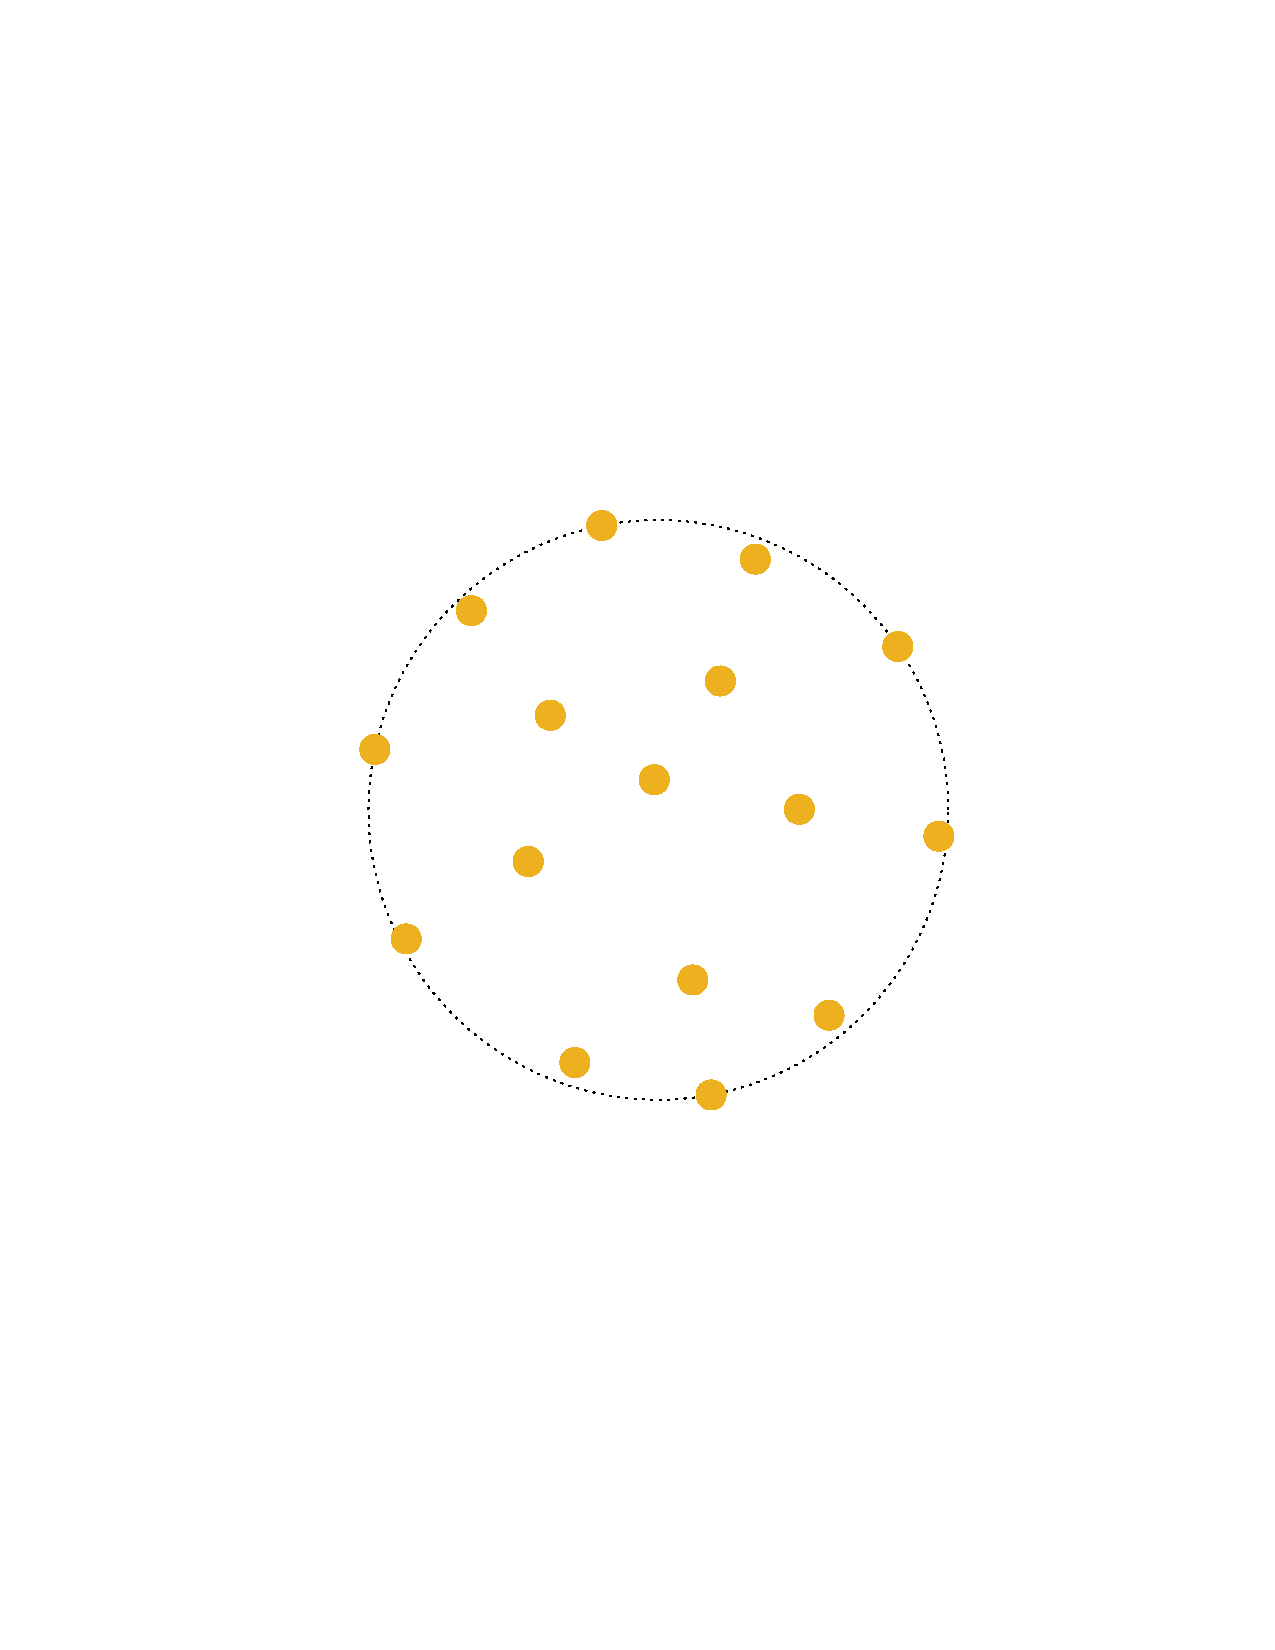
\includegraphics[clip, width=0.3\textwidth,scale=0.025, trim={3cm 8cm 3cm 8cm}]{figures/iea37-opt16-par2.pdf}
	}
	\subfigure[\textit{sub3}]{
		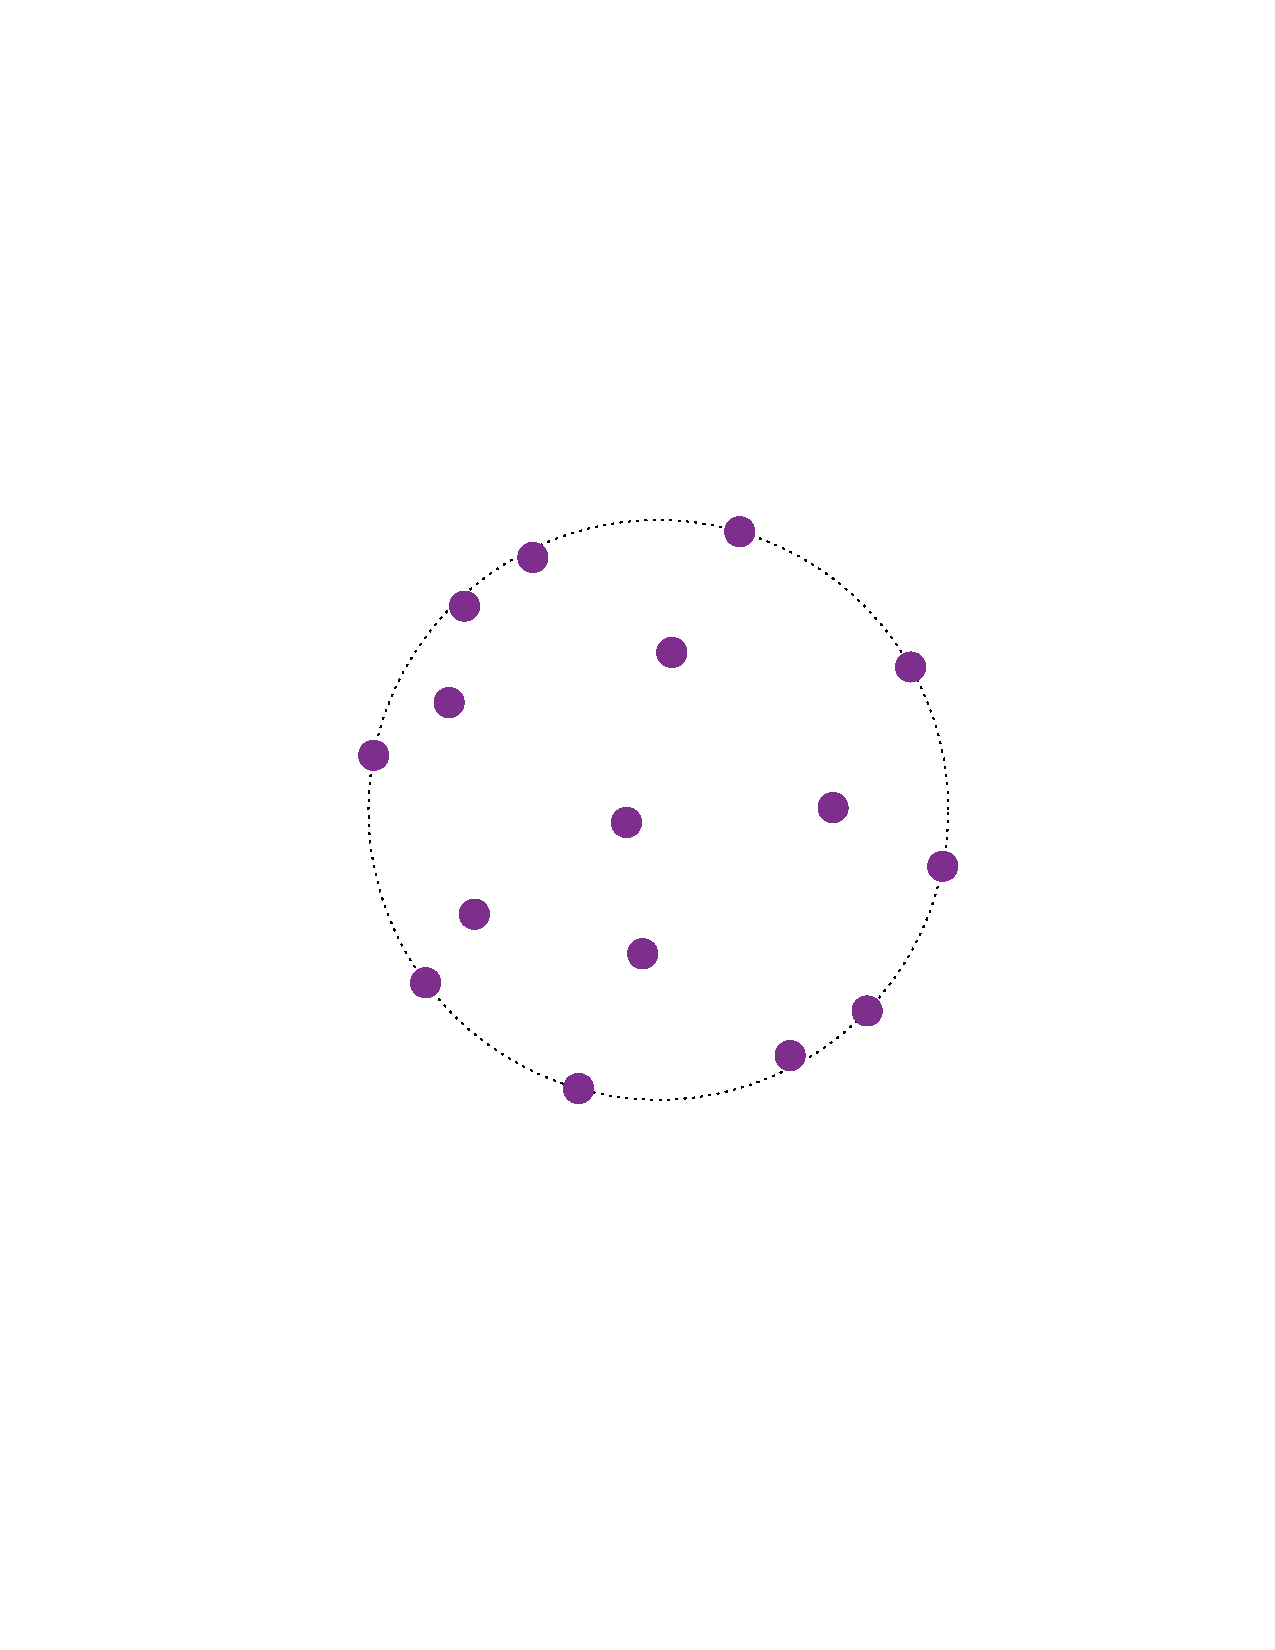
\includegraphics[clip, width=0.3\textwidth,scale=0.025, trim={3cm 8cm 3cm 8cm}]{figures/iea37-opt16-par3.pdf}
	}
	\subfigure[\textit{sub4}]{
		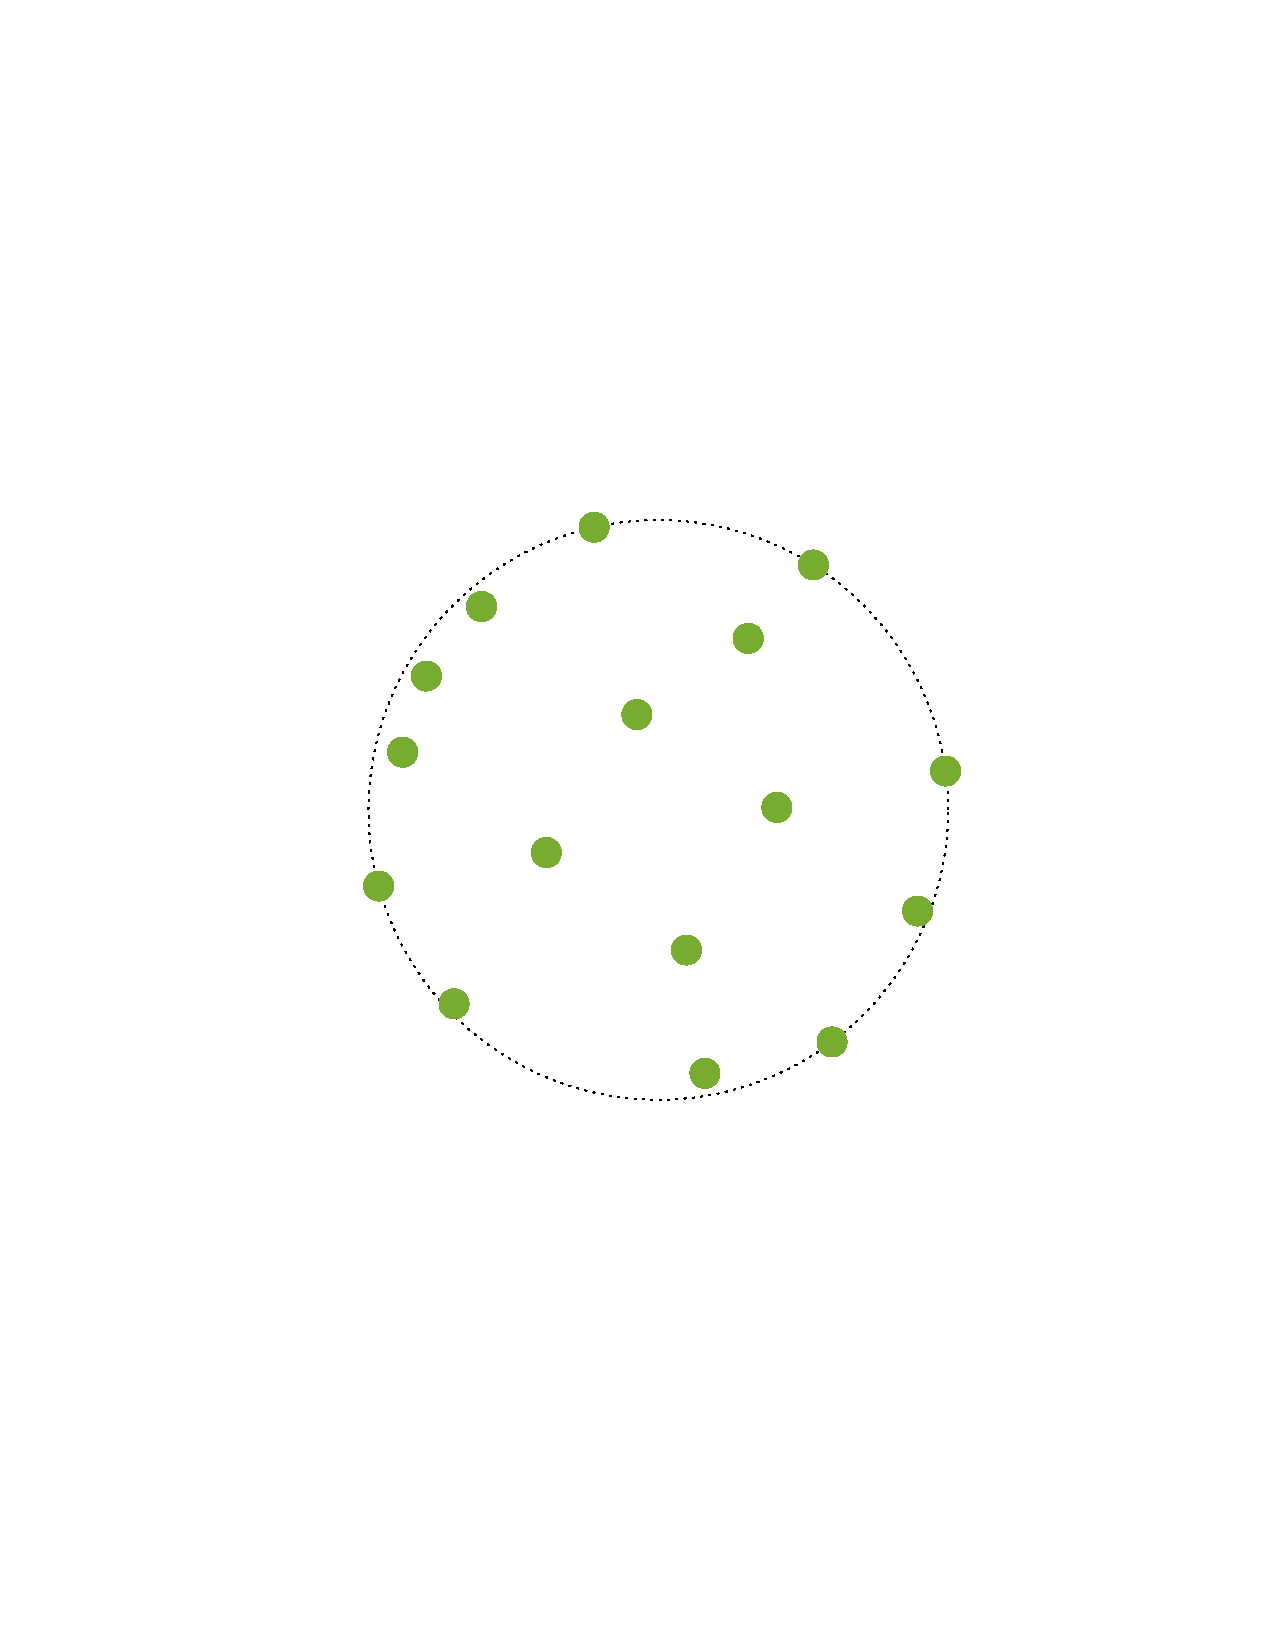
\includegraphics[clip, width=0.3\textwidth, scale=0.025, trim={3cm 8cm 3cm 8cm}]{figures/iea37-opt16-par4.pdf}
	}
	\subfigure[\textit{sub5}]{
		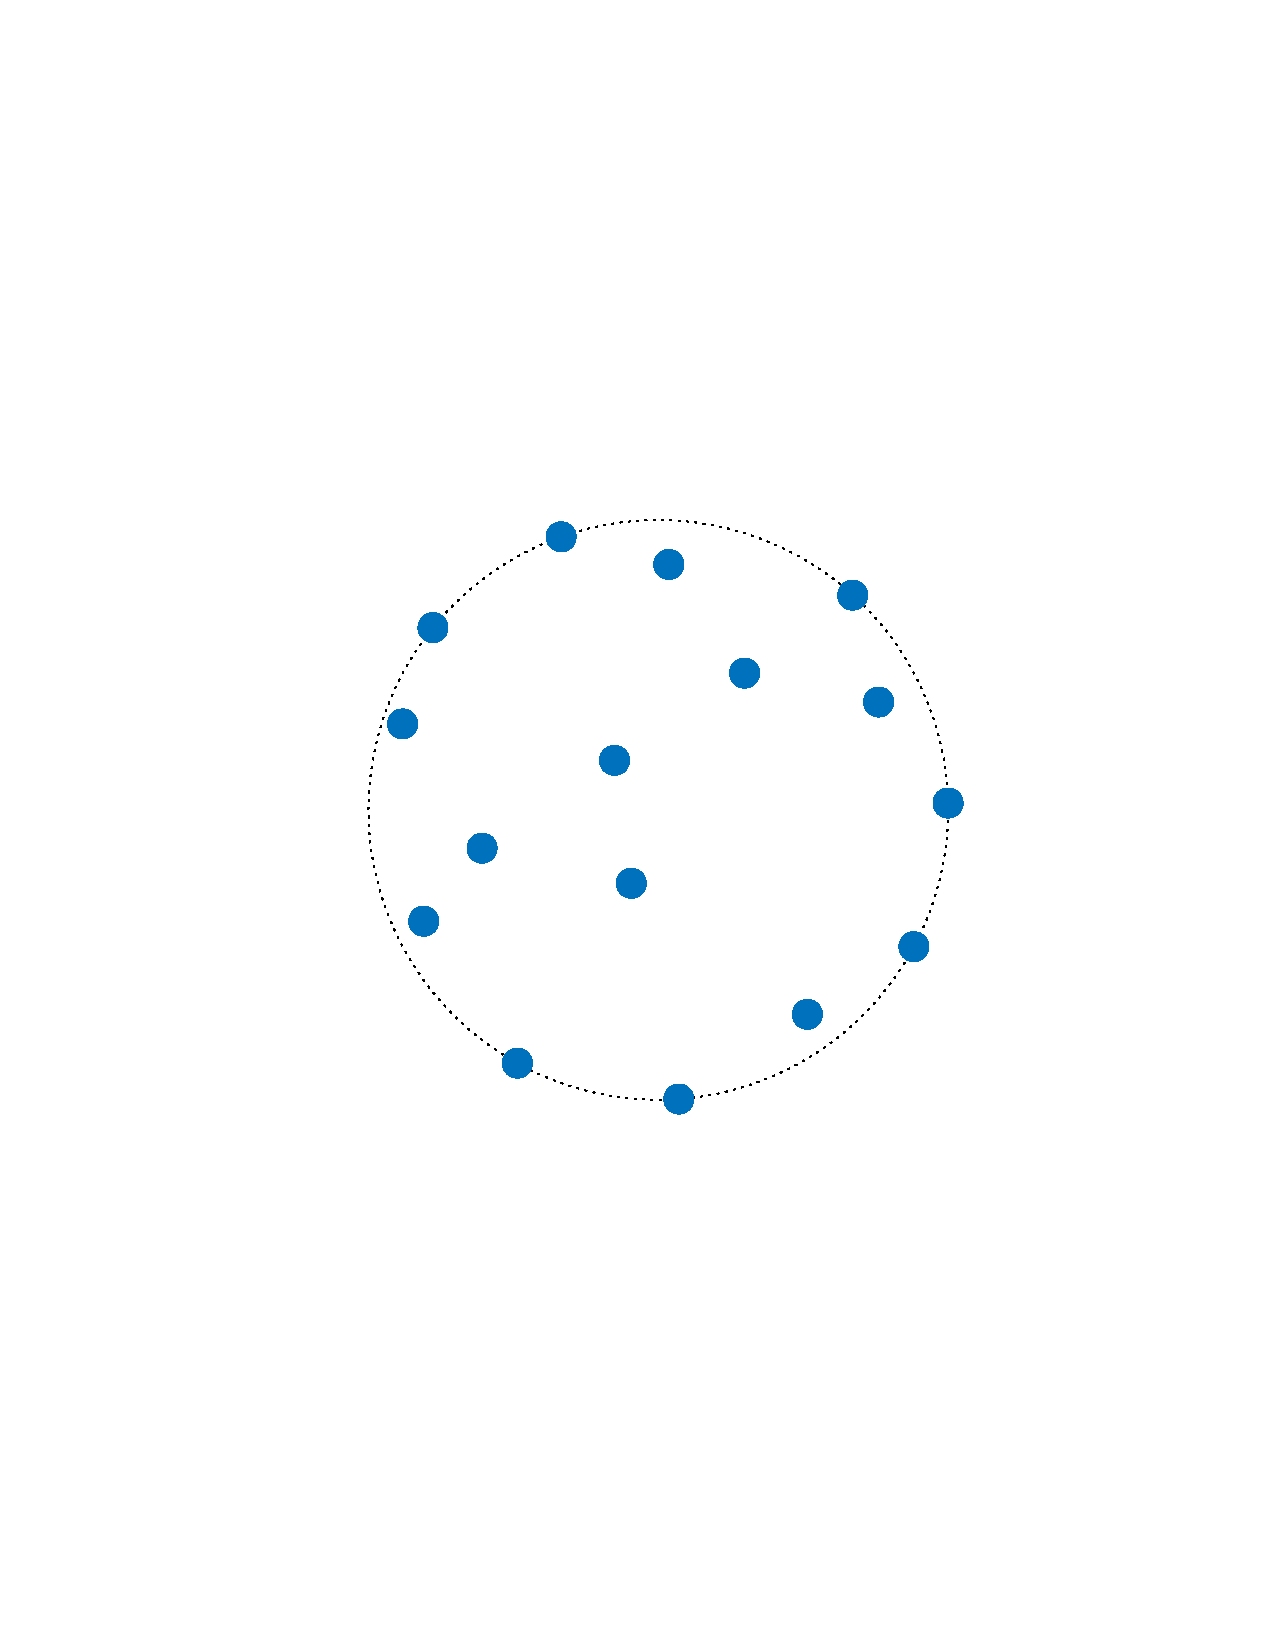
\includegraphics[clip, width=0.3\textwidth, scale=0.025, trim={3cm 8cm 3cm 8cm}]{figures/iea37-opt16-par5.pdf}
	}
	\subfigure[\textit{sub6}]{
		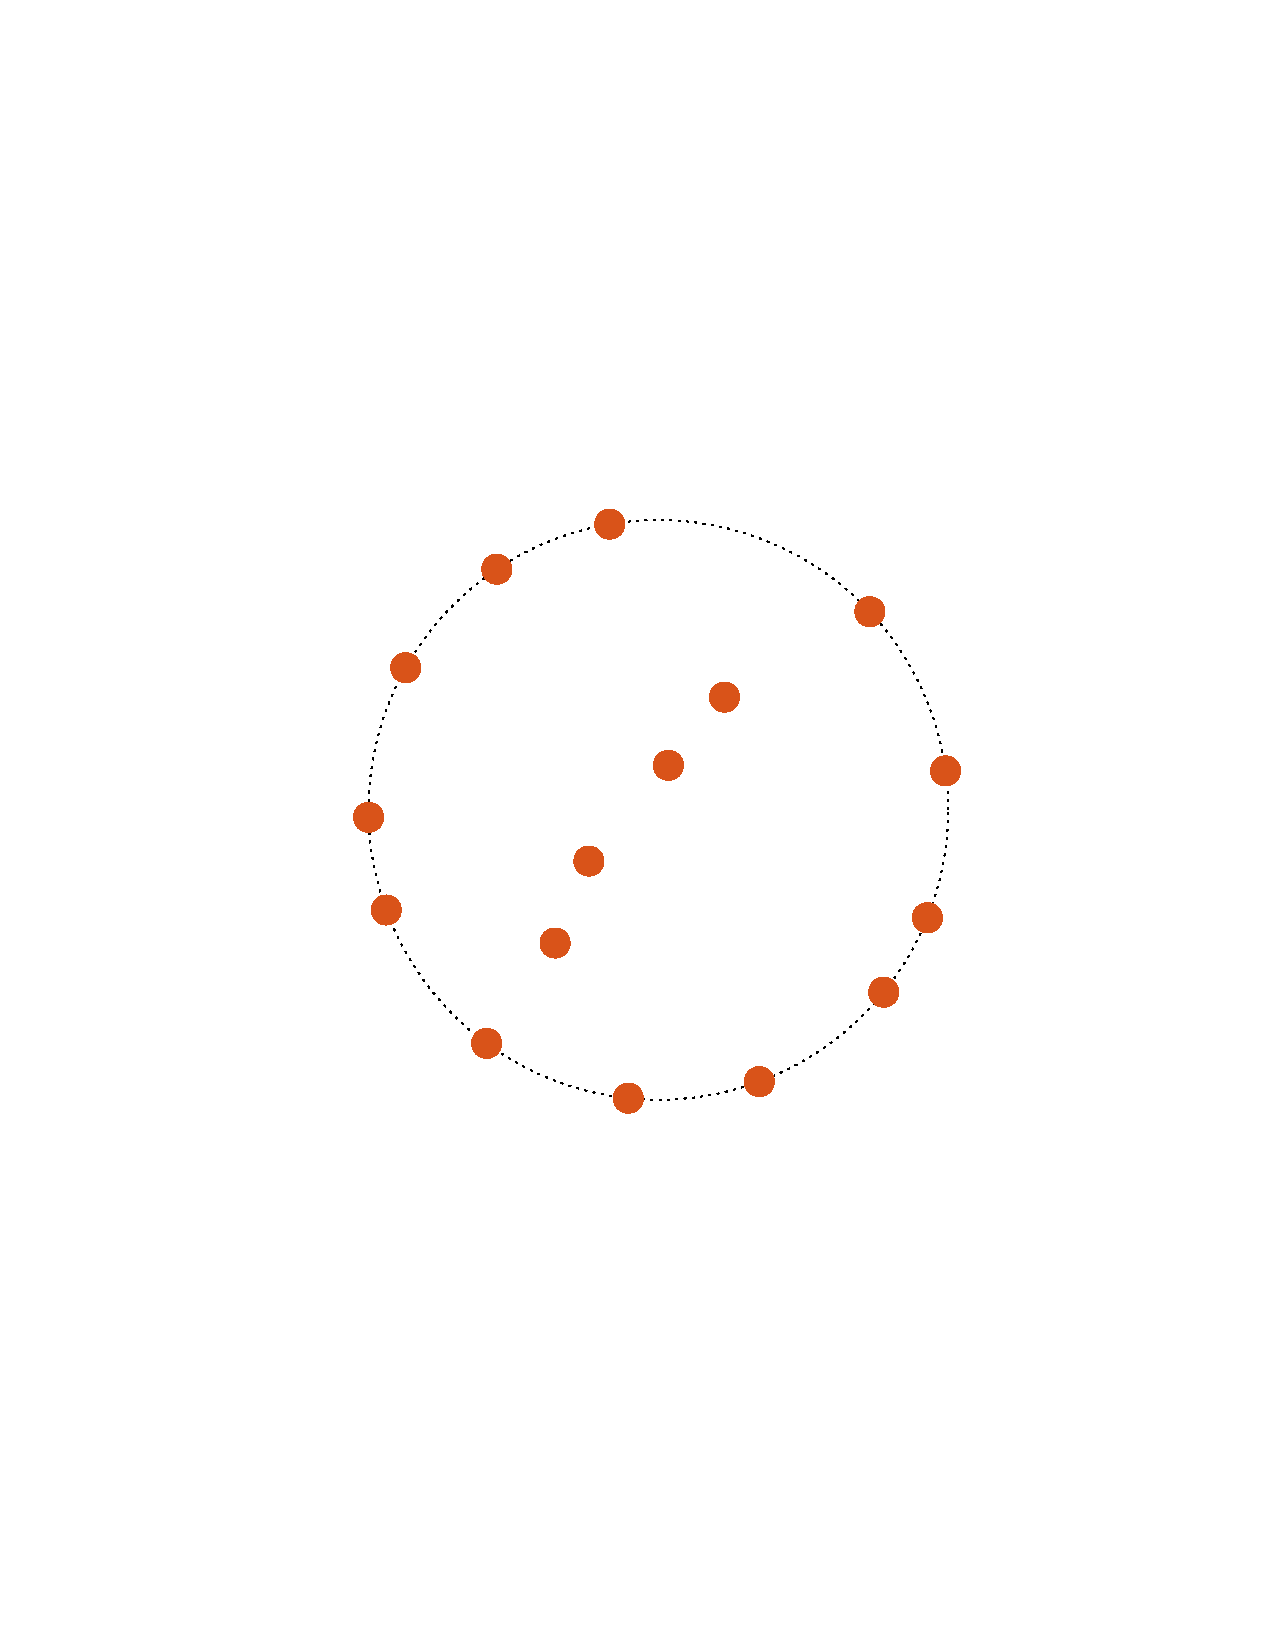
\includegraphics[clip, width=0.3\textwidth, scale=0.025, trim={3cm 8cm 3cm 8cm}]{figures/iea37-opt16-par6.pdf}
	}
	\subfigure[\textit{sub7}]{
		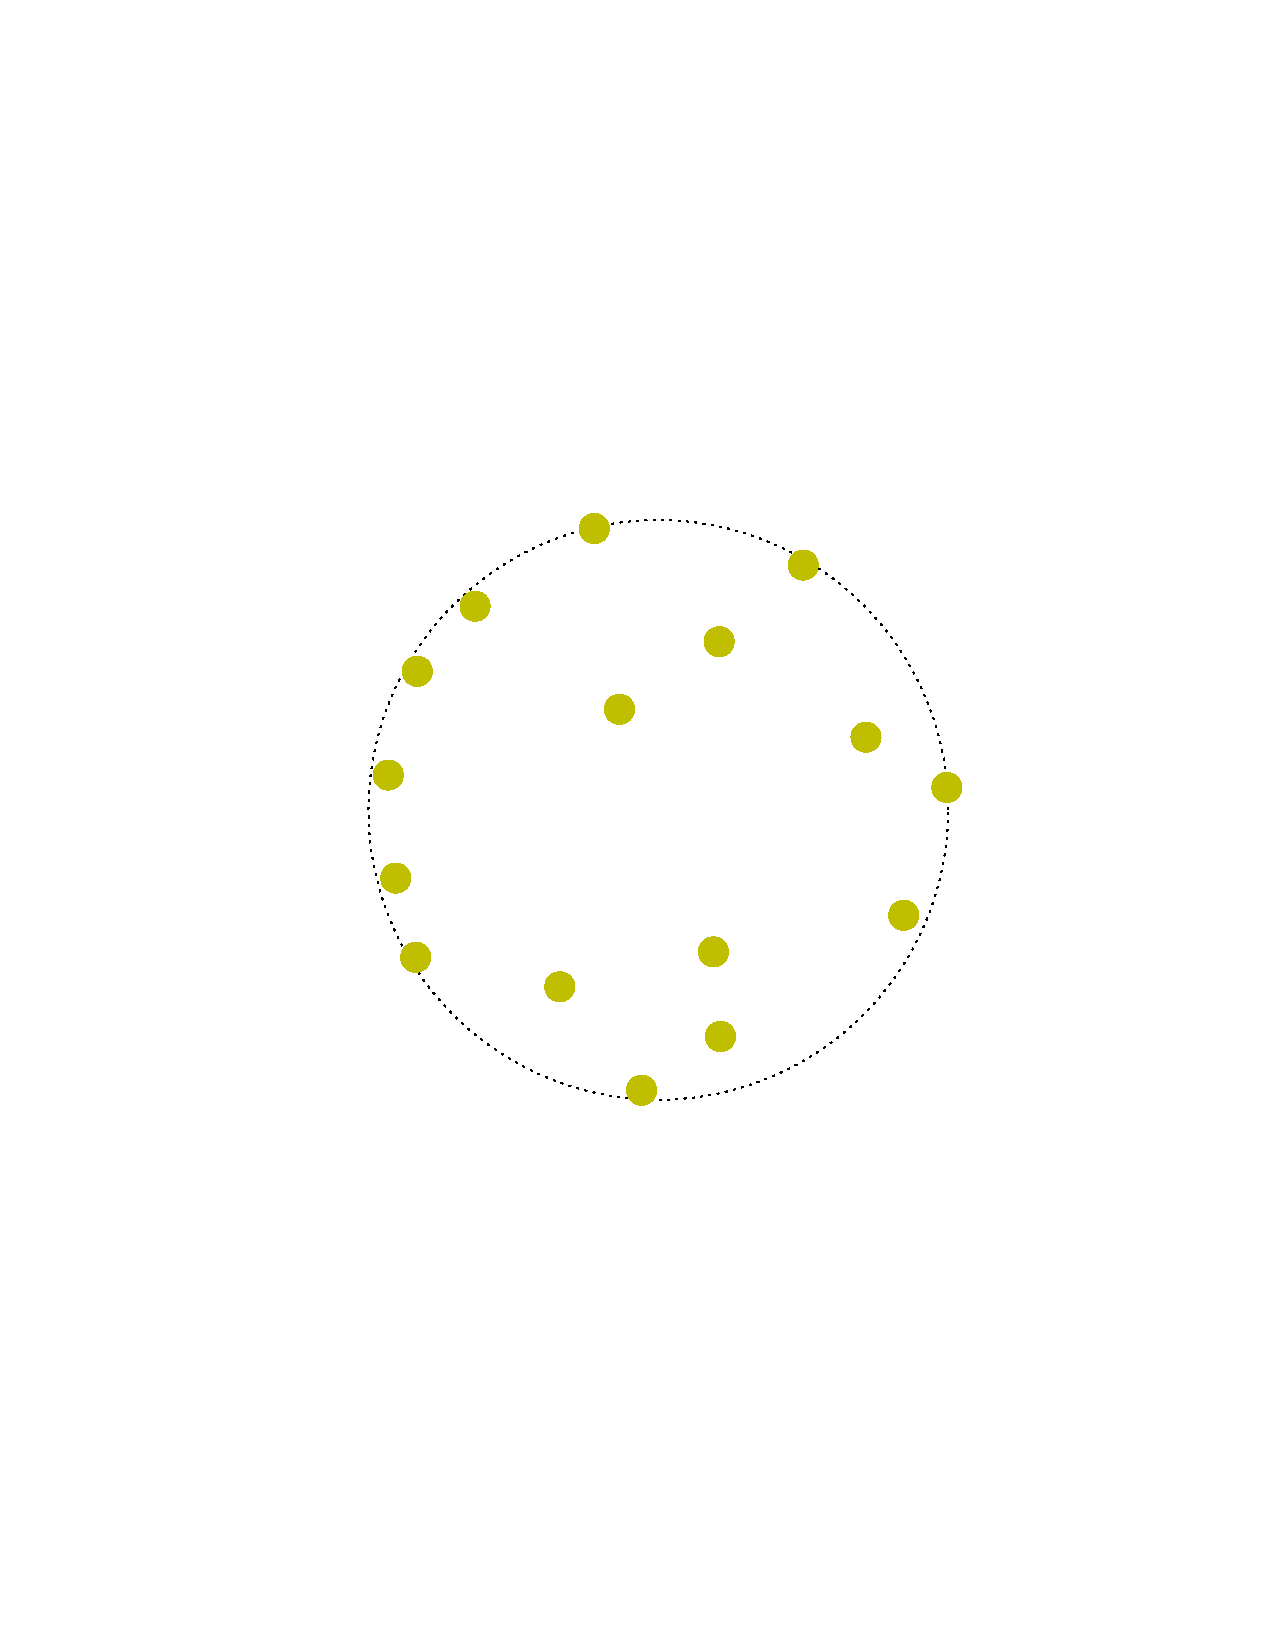
\includegraphics[clip, width=0.3\textwidth,scale=0.025, trim={3cm 8cm 3cm 8cm}]{figures/iea37-opt16-par7.pdf}
	}
	\subfigure[\textit{sub8}]{
		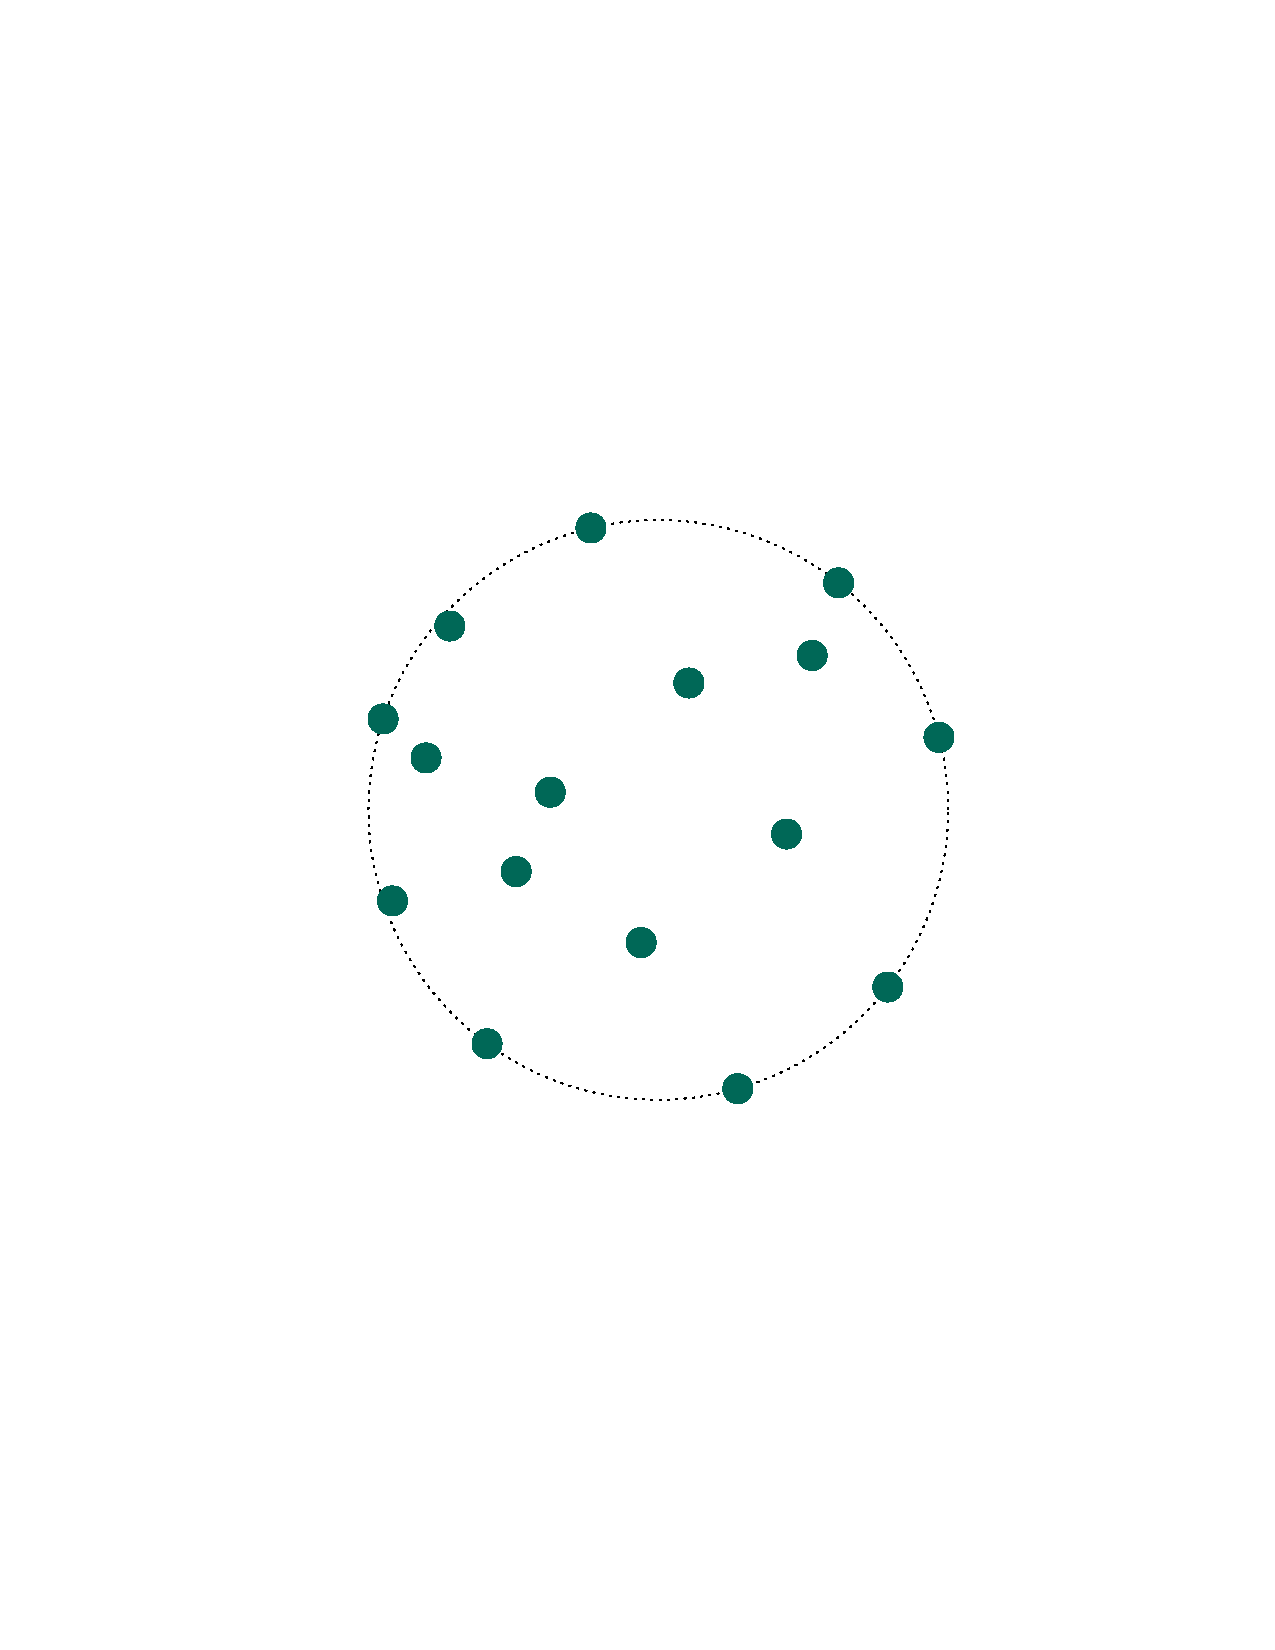
\includegraphics[clip, width=0.3\textwidth,scale=0.025, trim={3cm 8cm 3cm 8cm}]{figures/iea37-opt16-par8.pdf}
	}
	\subfigure[\textit{sub9}]{
		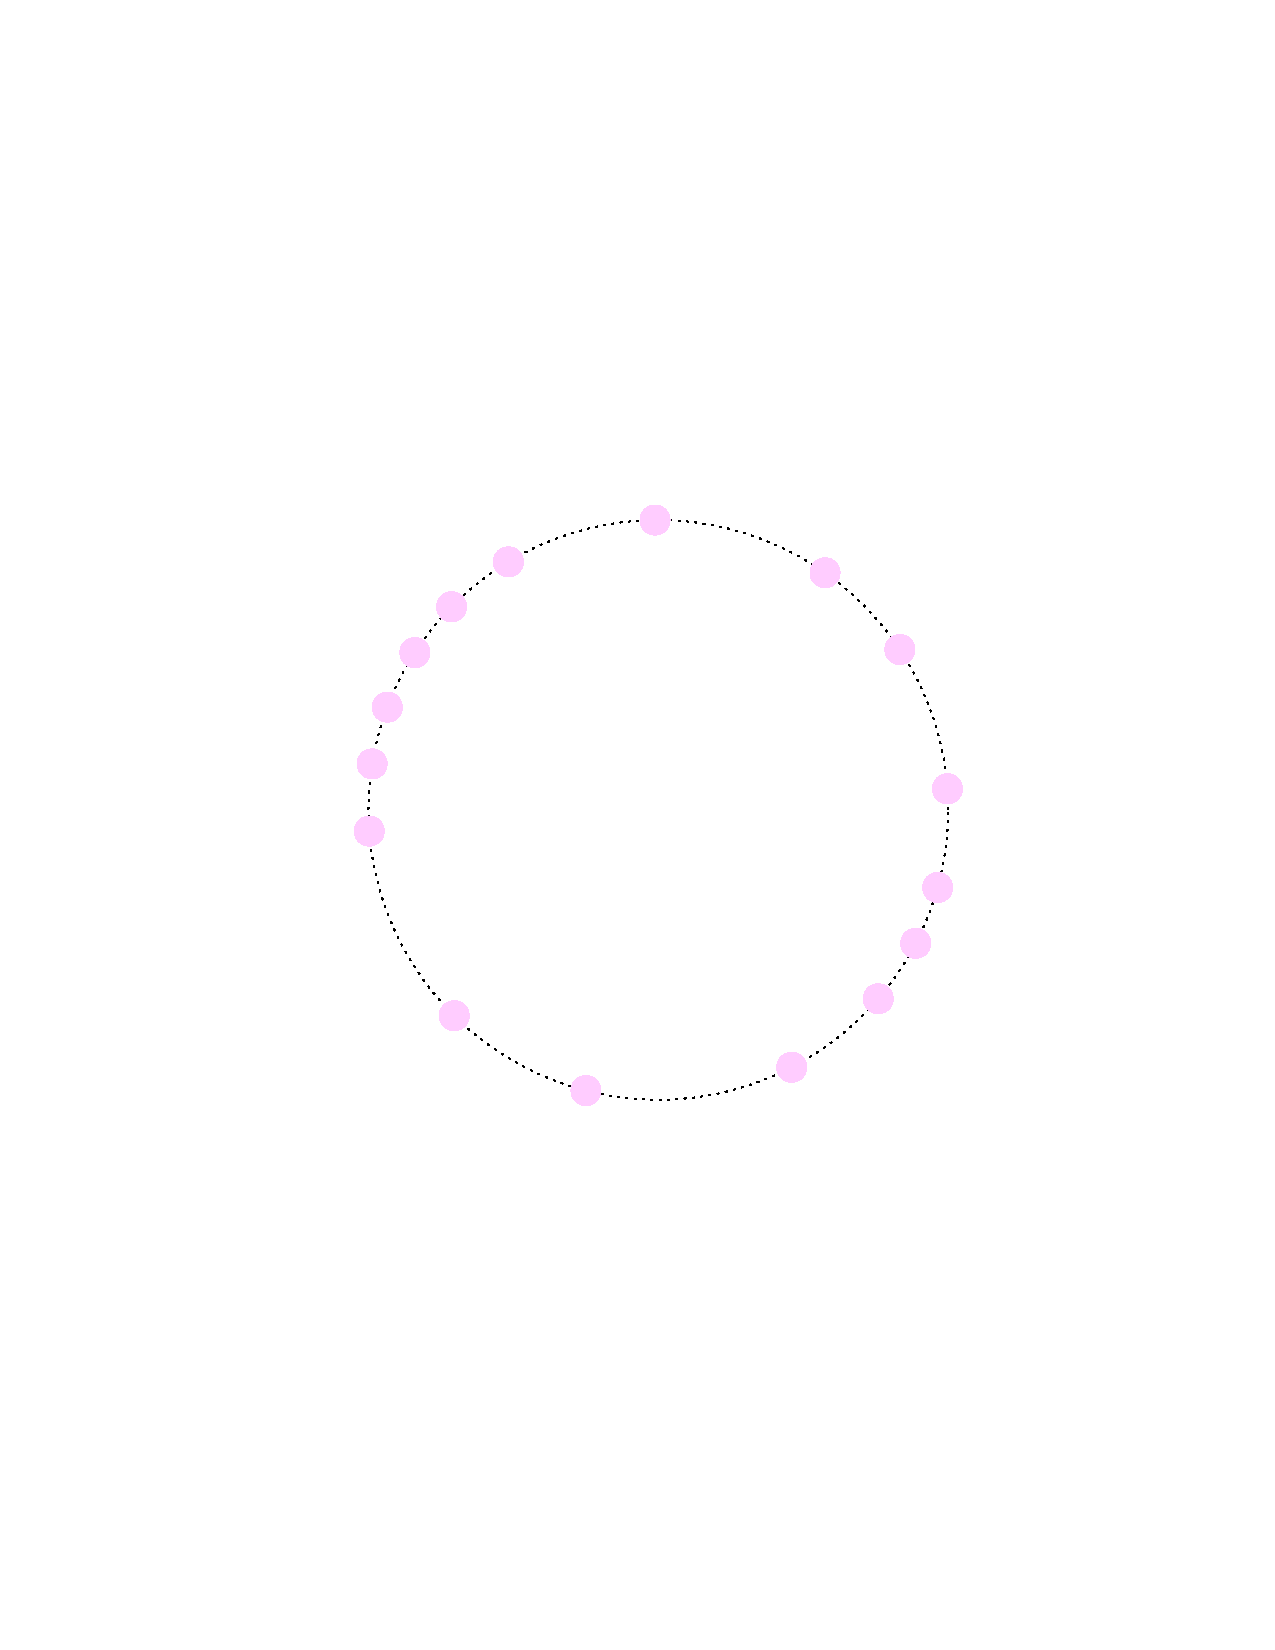
\includegraphics[clip, width=0.3\textwidth, scale=0.025, trim={3cm 8cm 3cm 8cm}]{figures/iea37-opt16-par9.pdf}
	}
	\subfigure[\textit{sub10}]{
		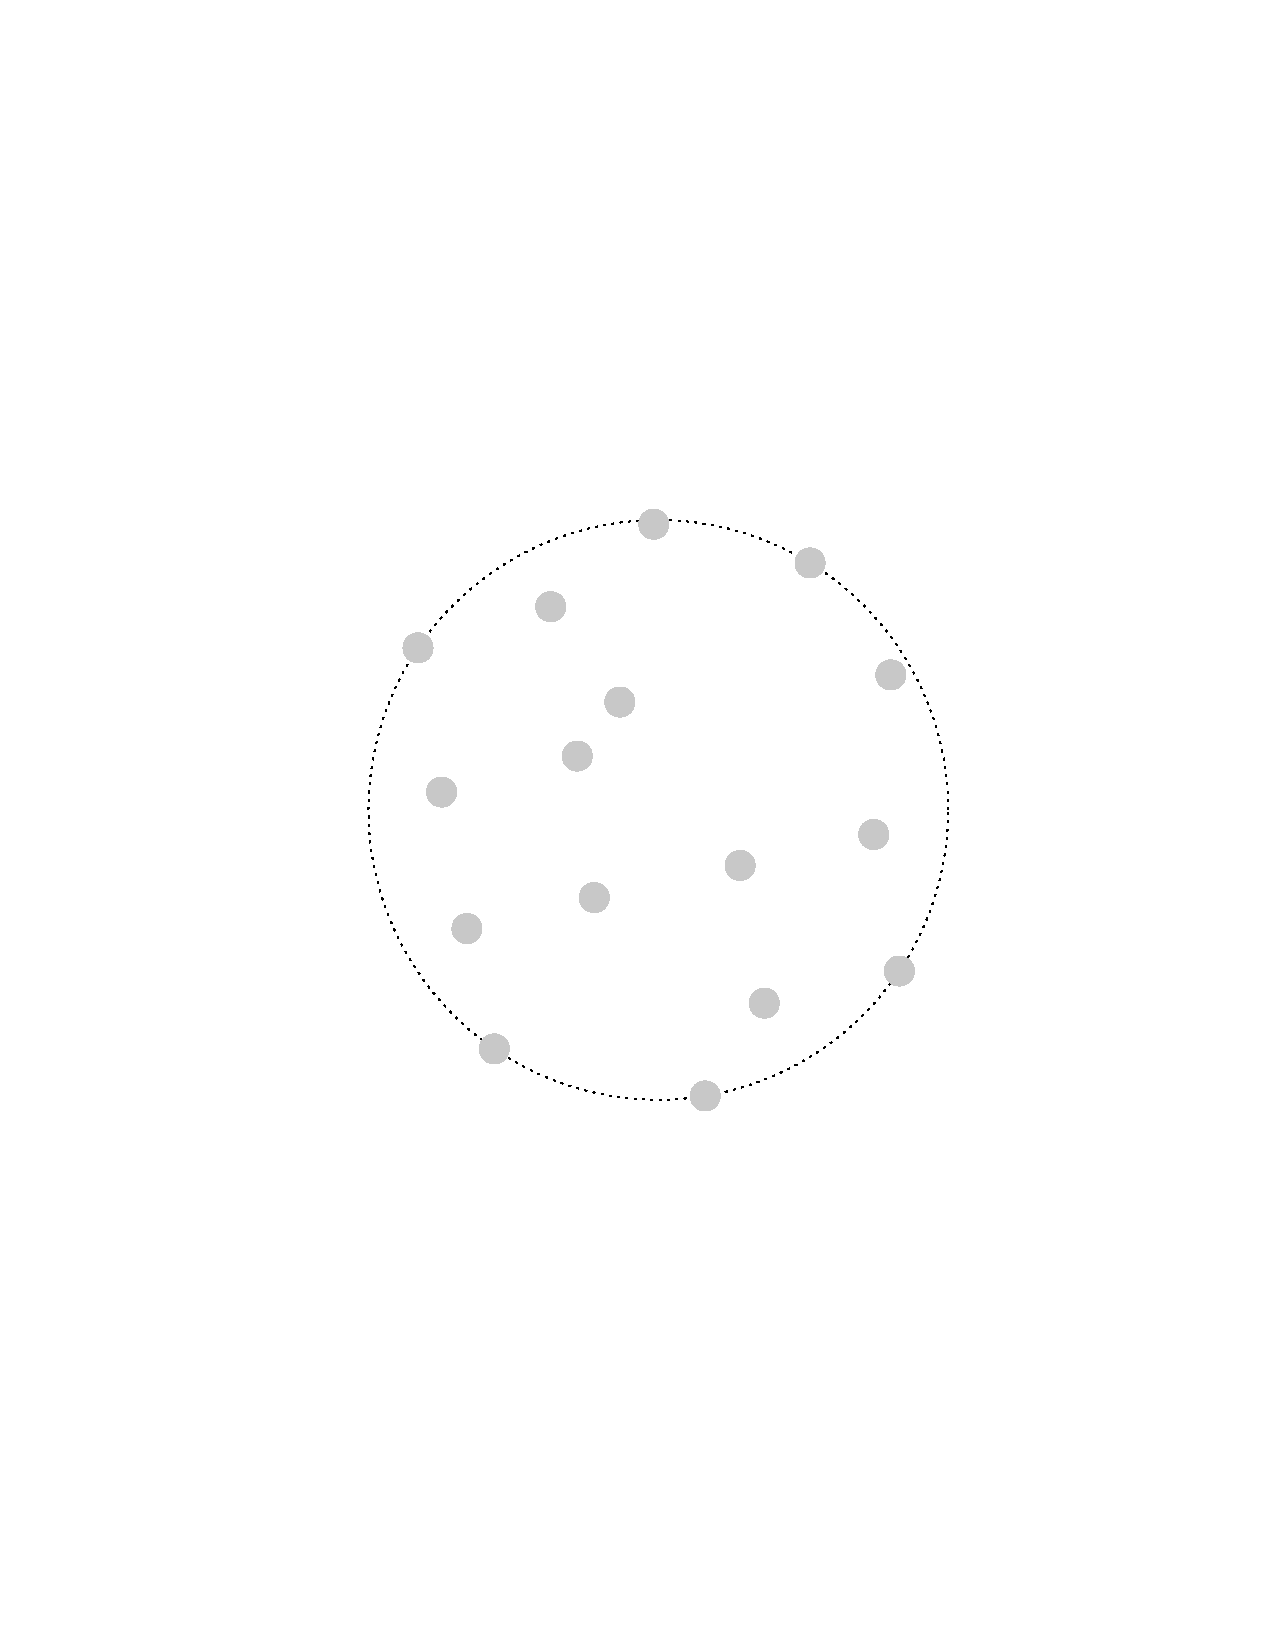
\includegraphics[clip, width=0.3\textwidth, scale=0.025, trim={3cm 8cm 3cm 8cm}]{figures/iea37-opt16-par10.pdf}
    }
    \subfigure[\textit{sub11}]{
		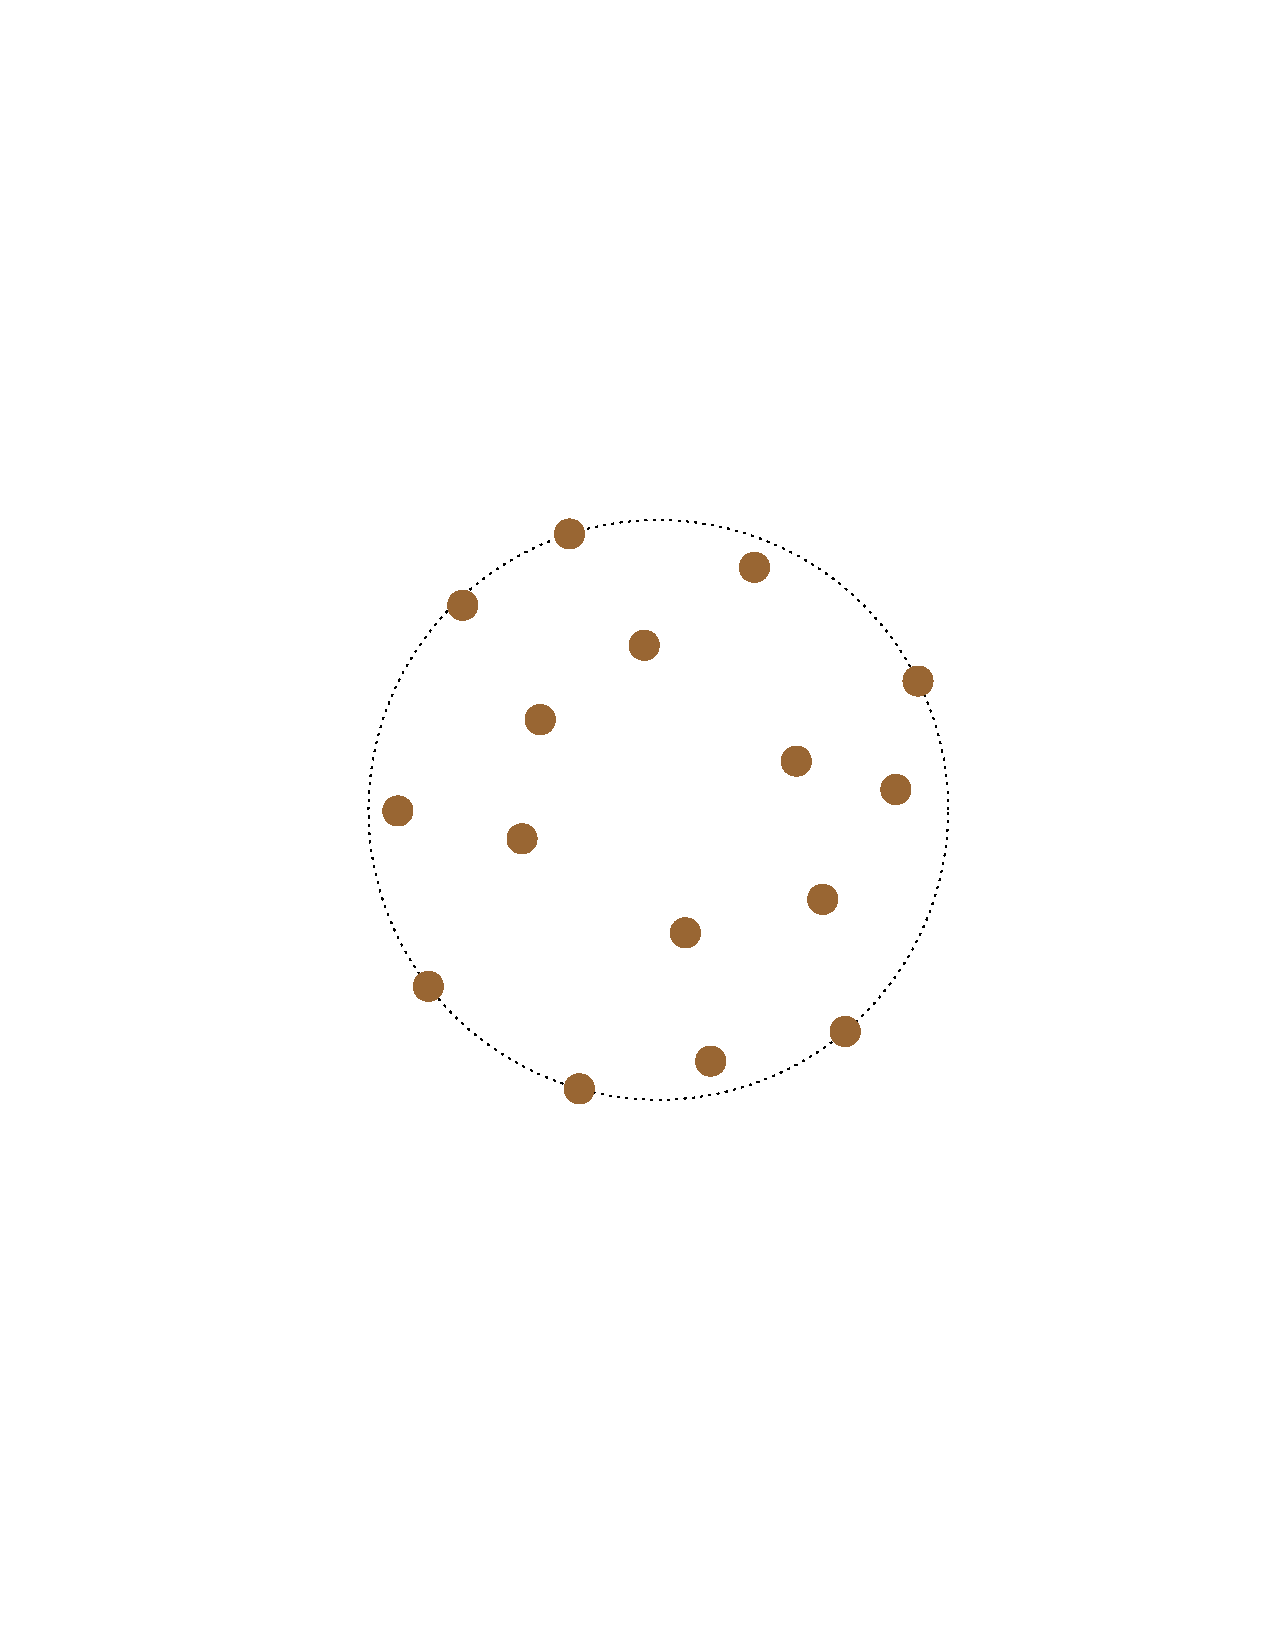
\includegraphics[clip, width=0.3\textwidth, scale=0.025, trim={3cm 8cm 3cm 8cm}]{figures/iea37-opt16-par11.pdf}
	}
	\subfigure[\textit{sub12}]{
		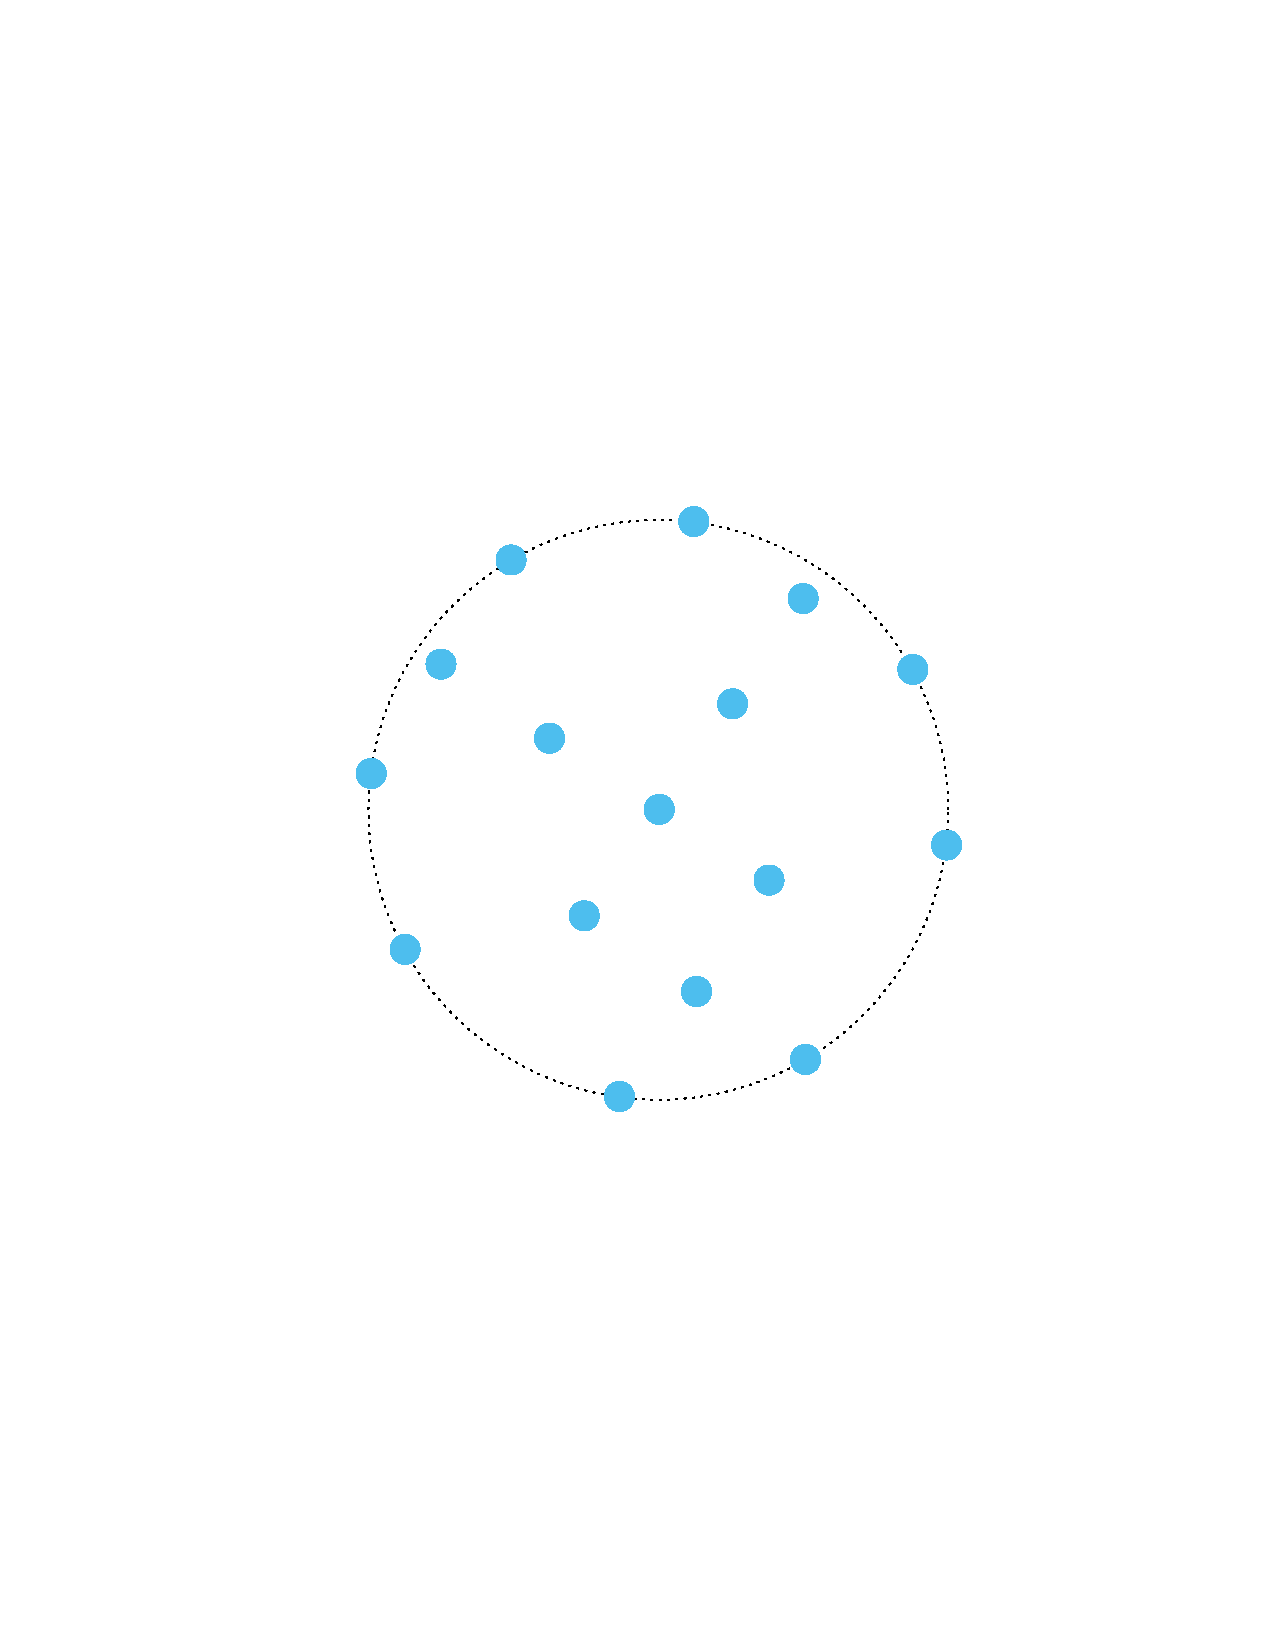
\includegraphics[clip, width=0.3\textwidth, scale=0.025, trim={3cm 8cm 3cm 8cm}]{figures/iea37-opt16-par12.pdf}
	}
	\caption{Case study 1: optimized wind farm layouts with 16 wind turbines.}
	\label{fig:16turbs}
\end{figure}

\begin{figure}[htbp!]
	\centering
	\subfigure[\textit{sub1}]{
		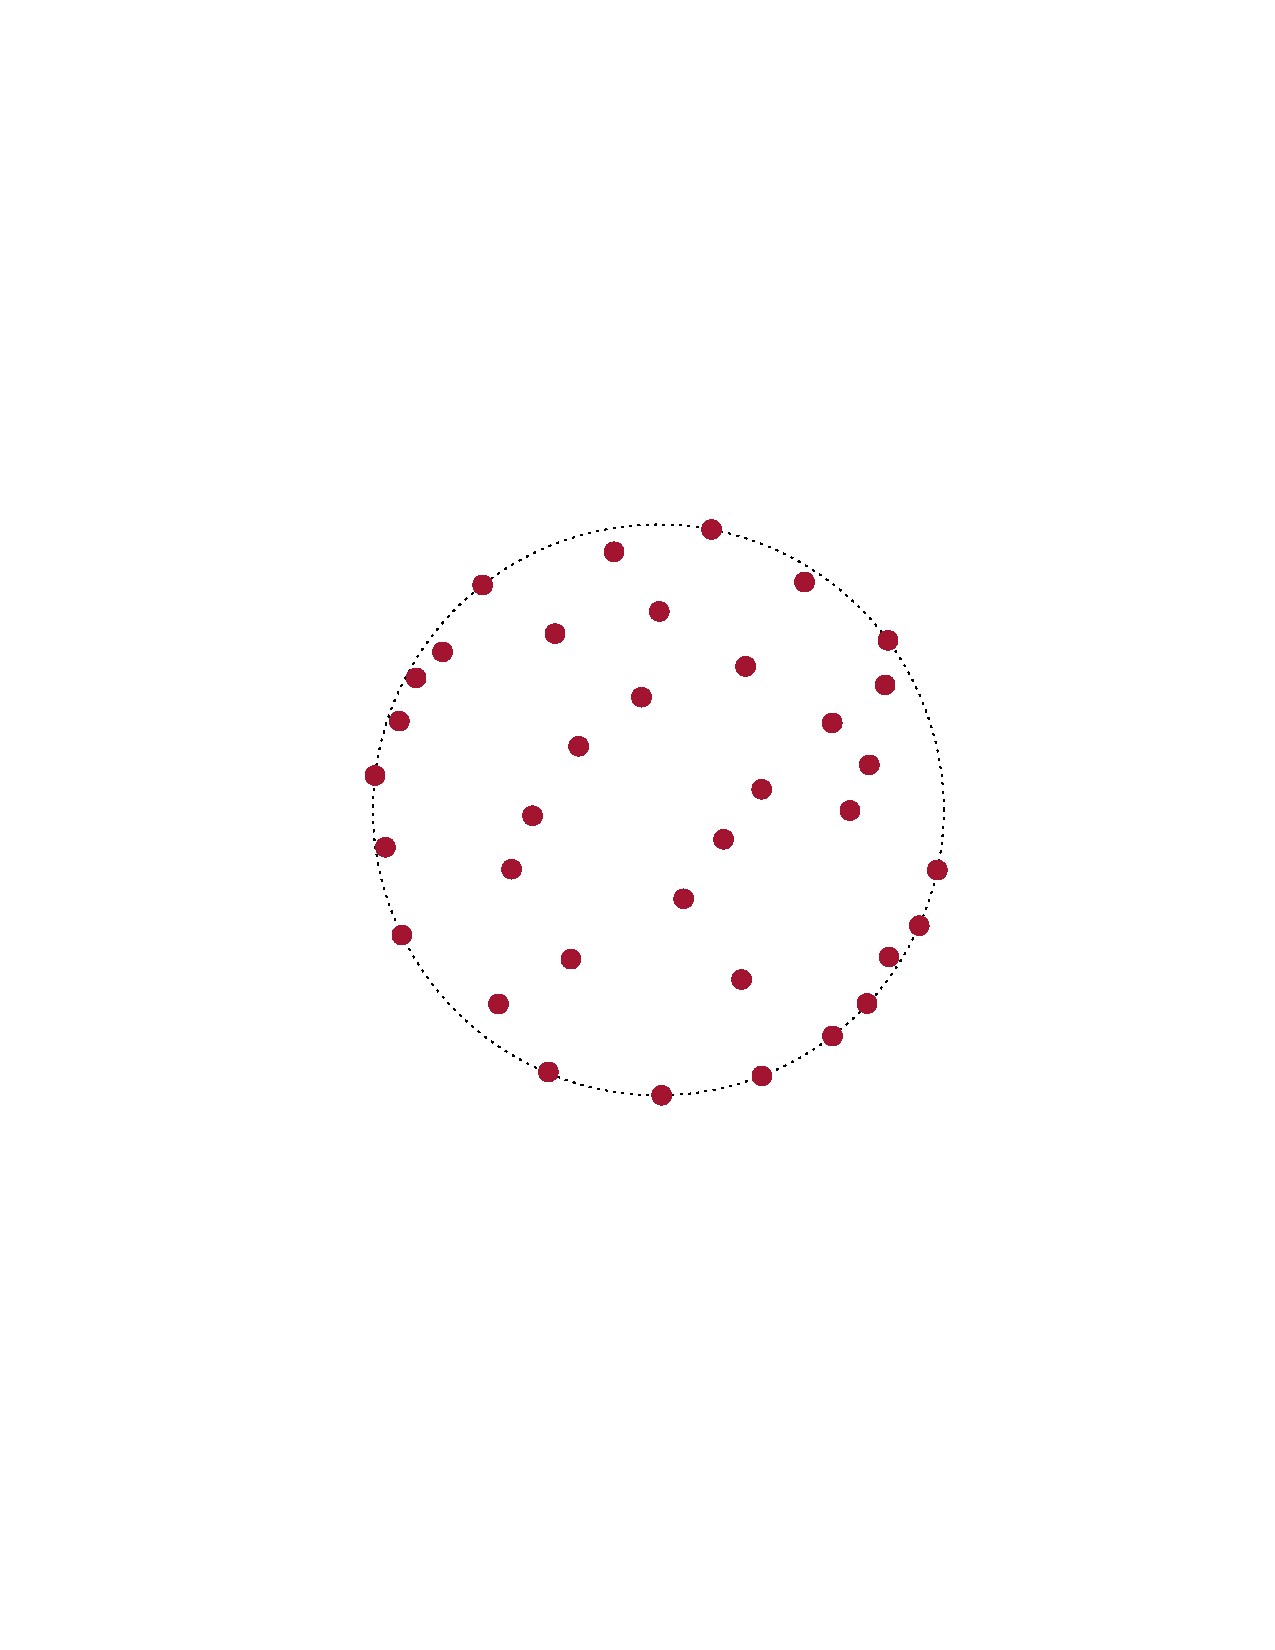
\includegraphics[clip, width=0.3\textwidth, scale=0.025, trim={3cm 8cm 3cm 8cm}]{figures/iea37-opt36-par1.pdf}
	}
	\subfigure[\textit{sub2}]{
		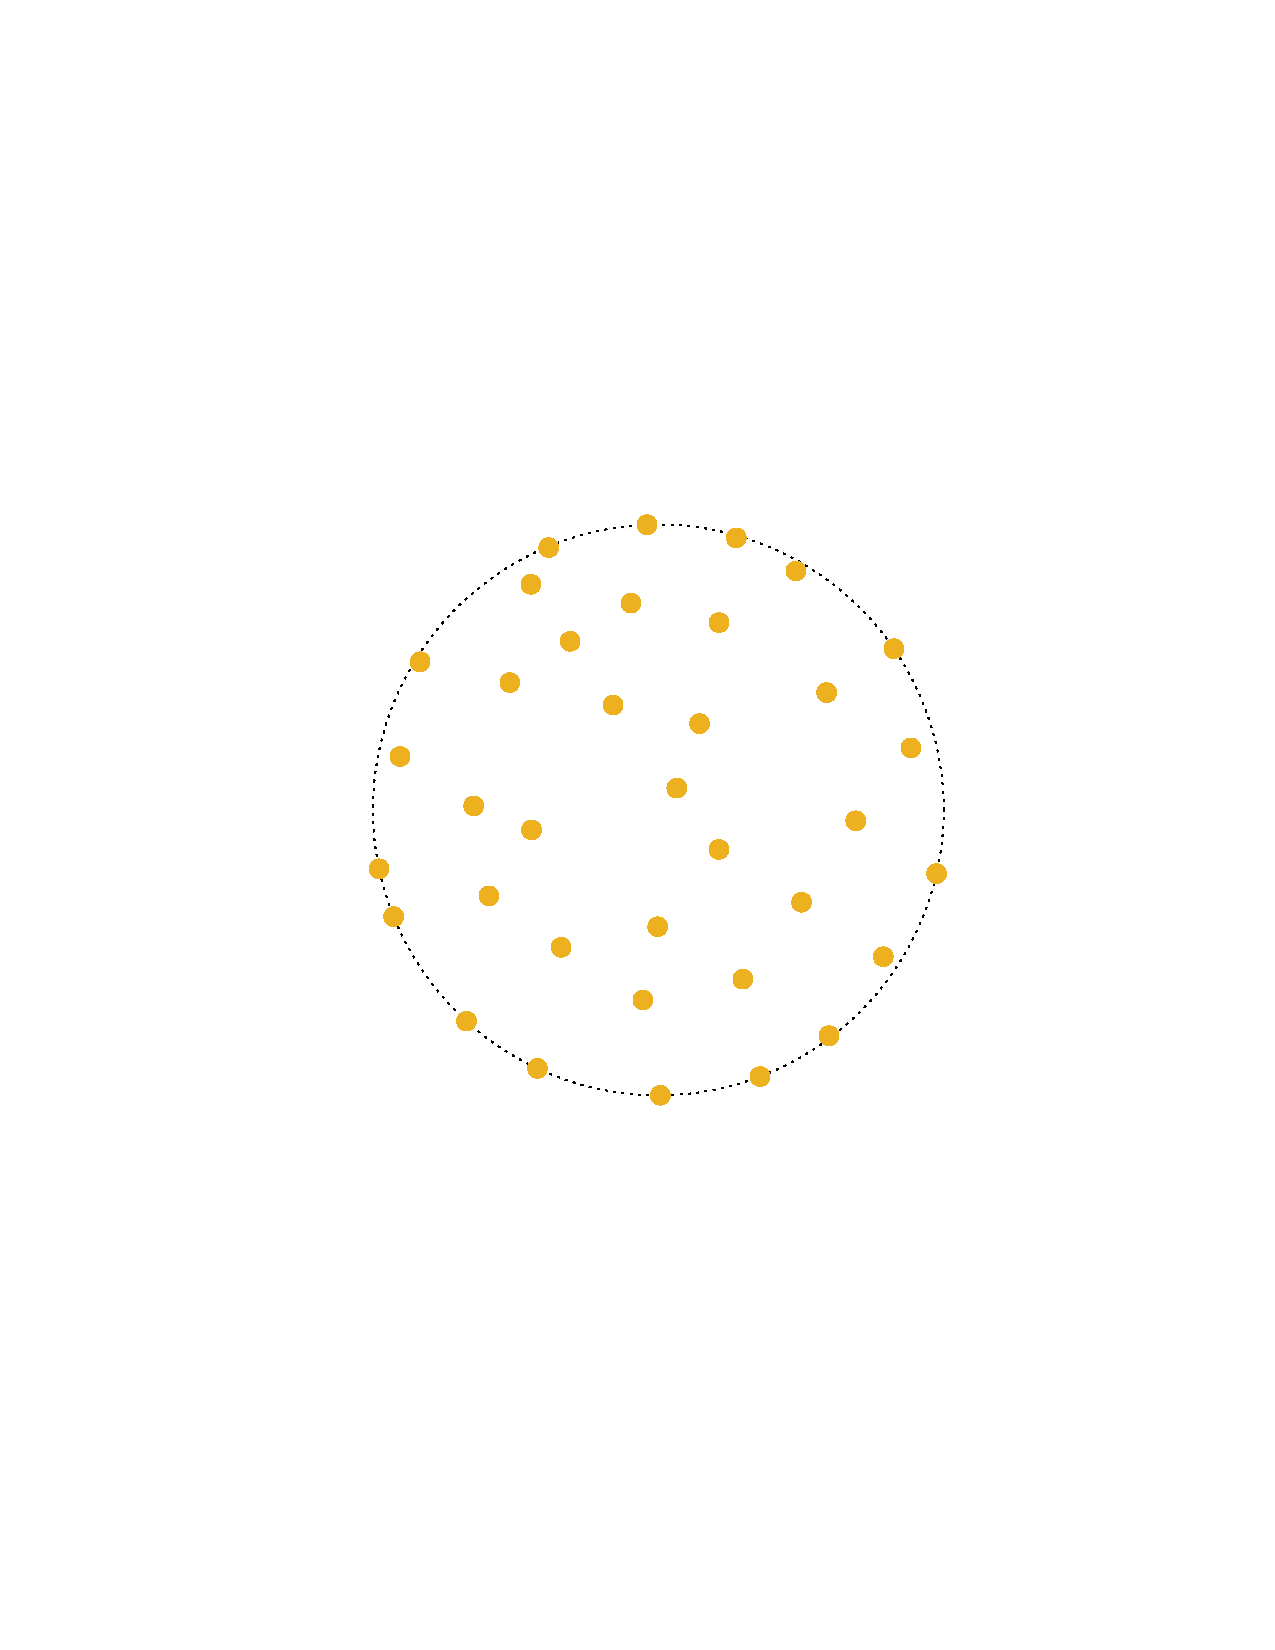
\includegraphics[clip, width=0.3\textwidth,scale=0.025, trim={3cm 8cm 3cm 8cm}]{figures/iea37-opt36-par2.pdf}
	}
	\subfigure[\textit{sub3}]{
		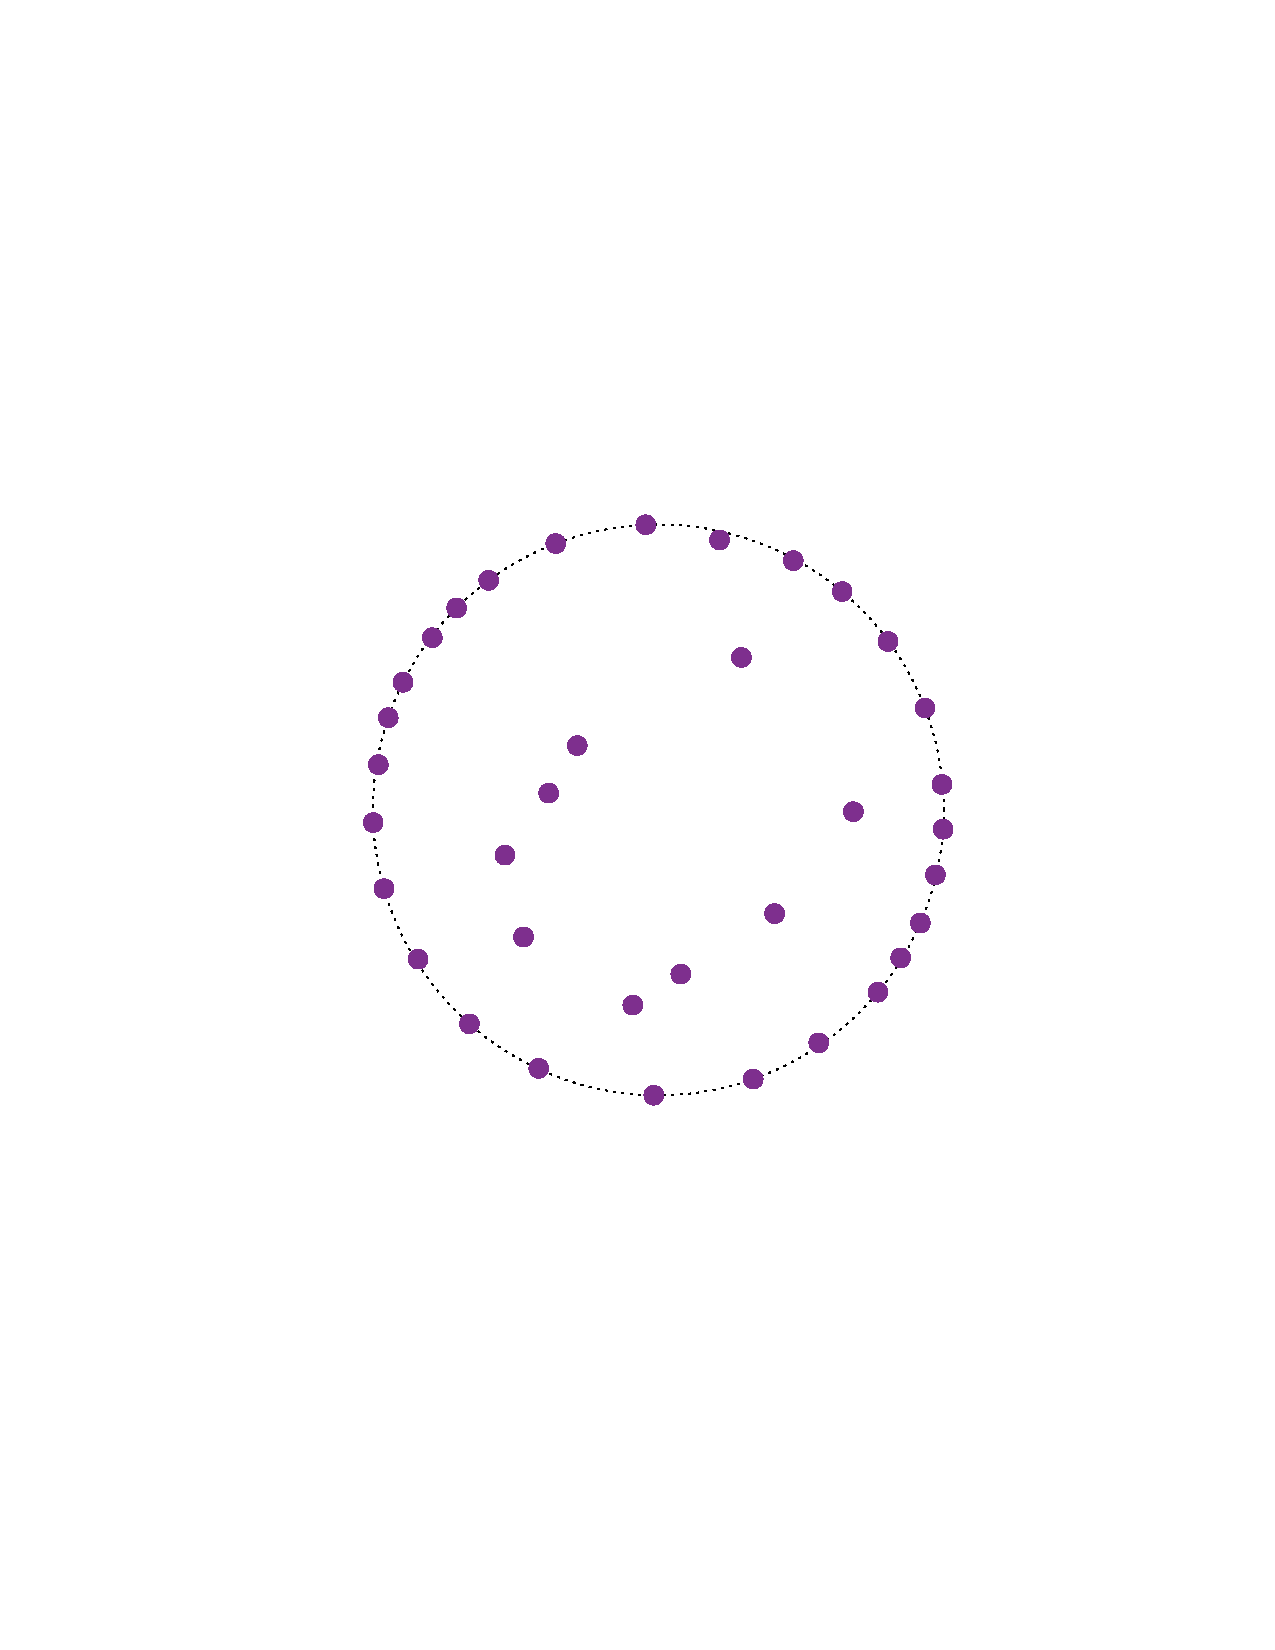
\includegraphics[clip, width=0.3\textwidth,scale=0.025, trim={3cm 8cm 3cm 8cm}]{figures/iea37-opt36-par3.pdf}
	}
	\subfigure[\textit{sub4}]{
		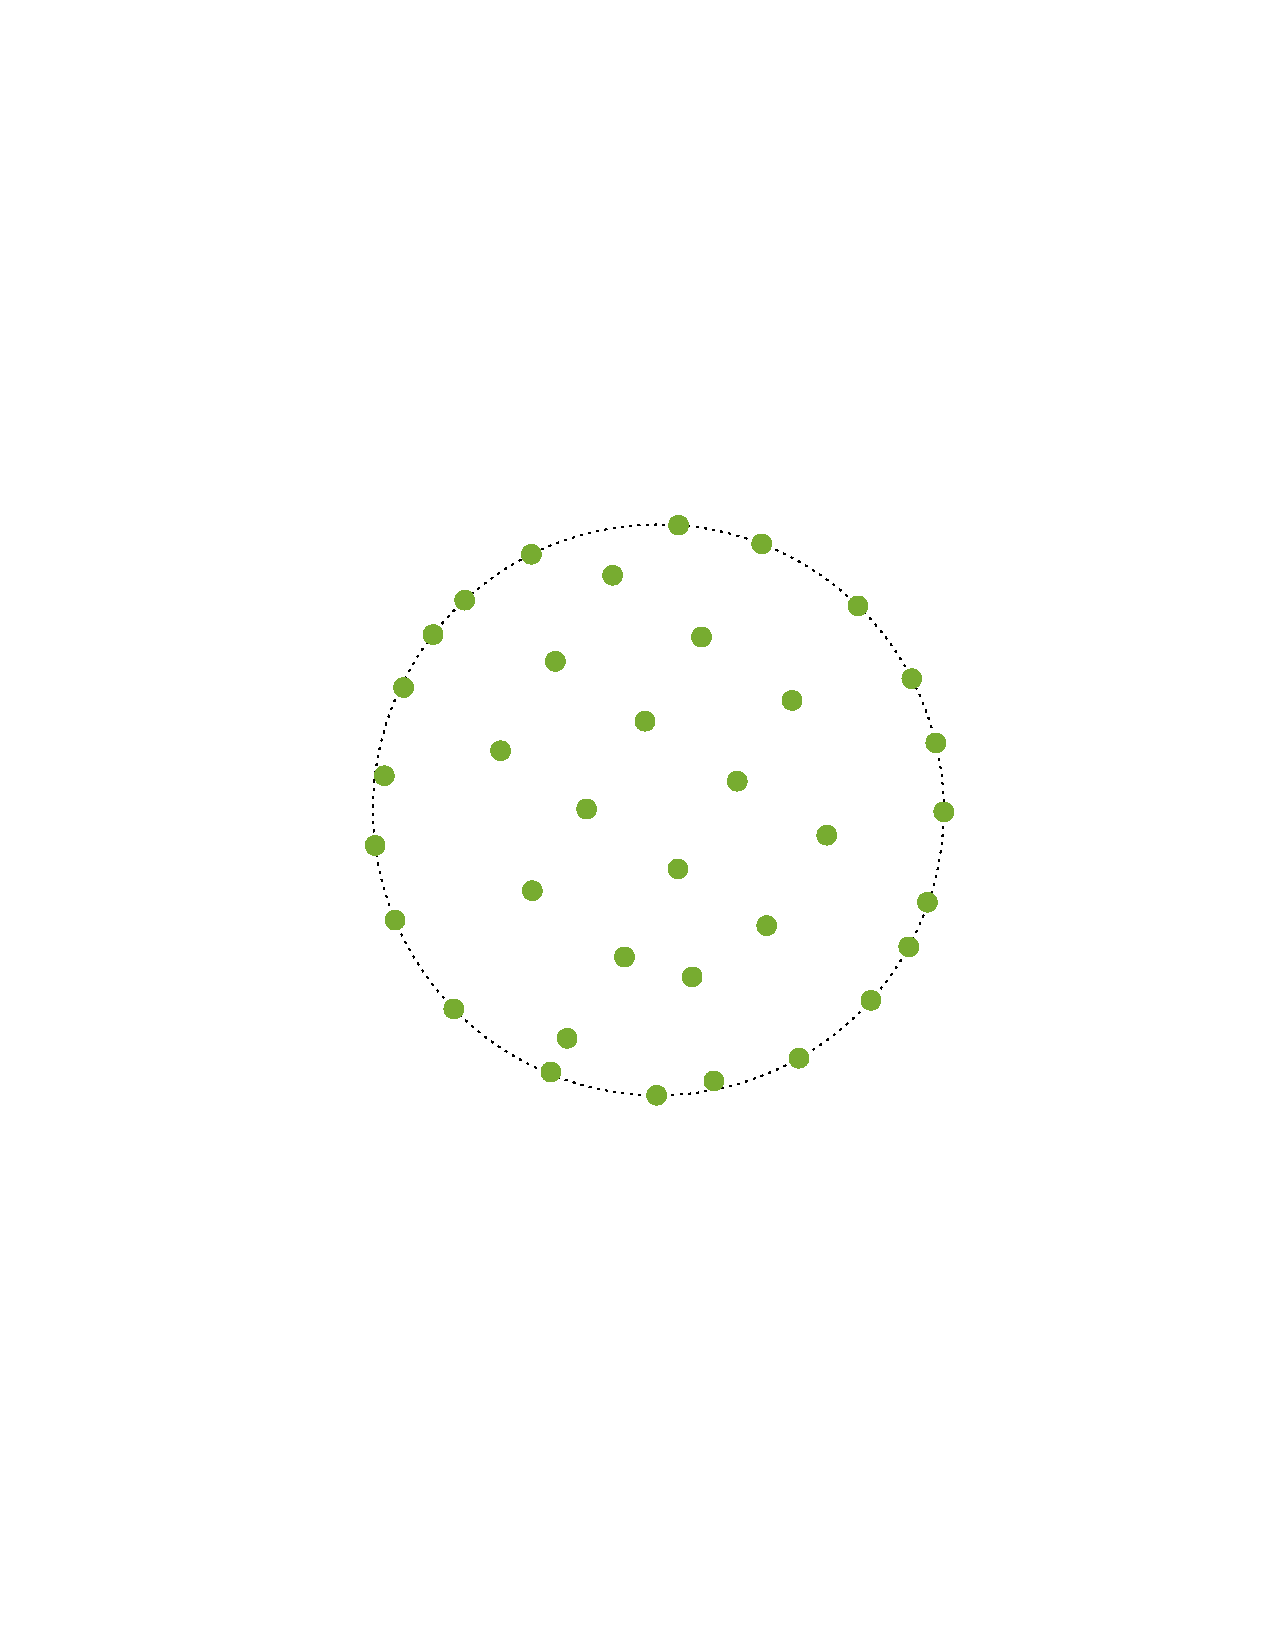
\includegraphics[clip, width=0.3\textwidth, scale=0.025, trim={3cm 8cm 3cm 8cm}]{figures/iea37-opt36-par4.pdf}
	}
	\subfigure[\textit{sub5}]{
		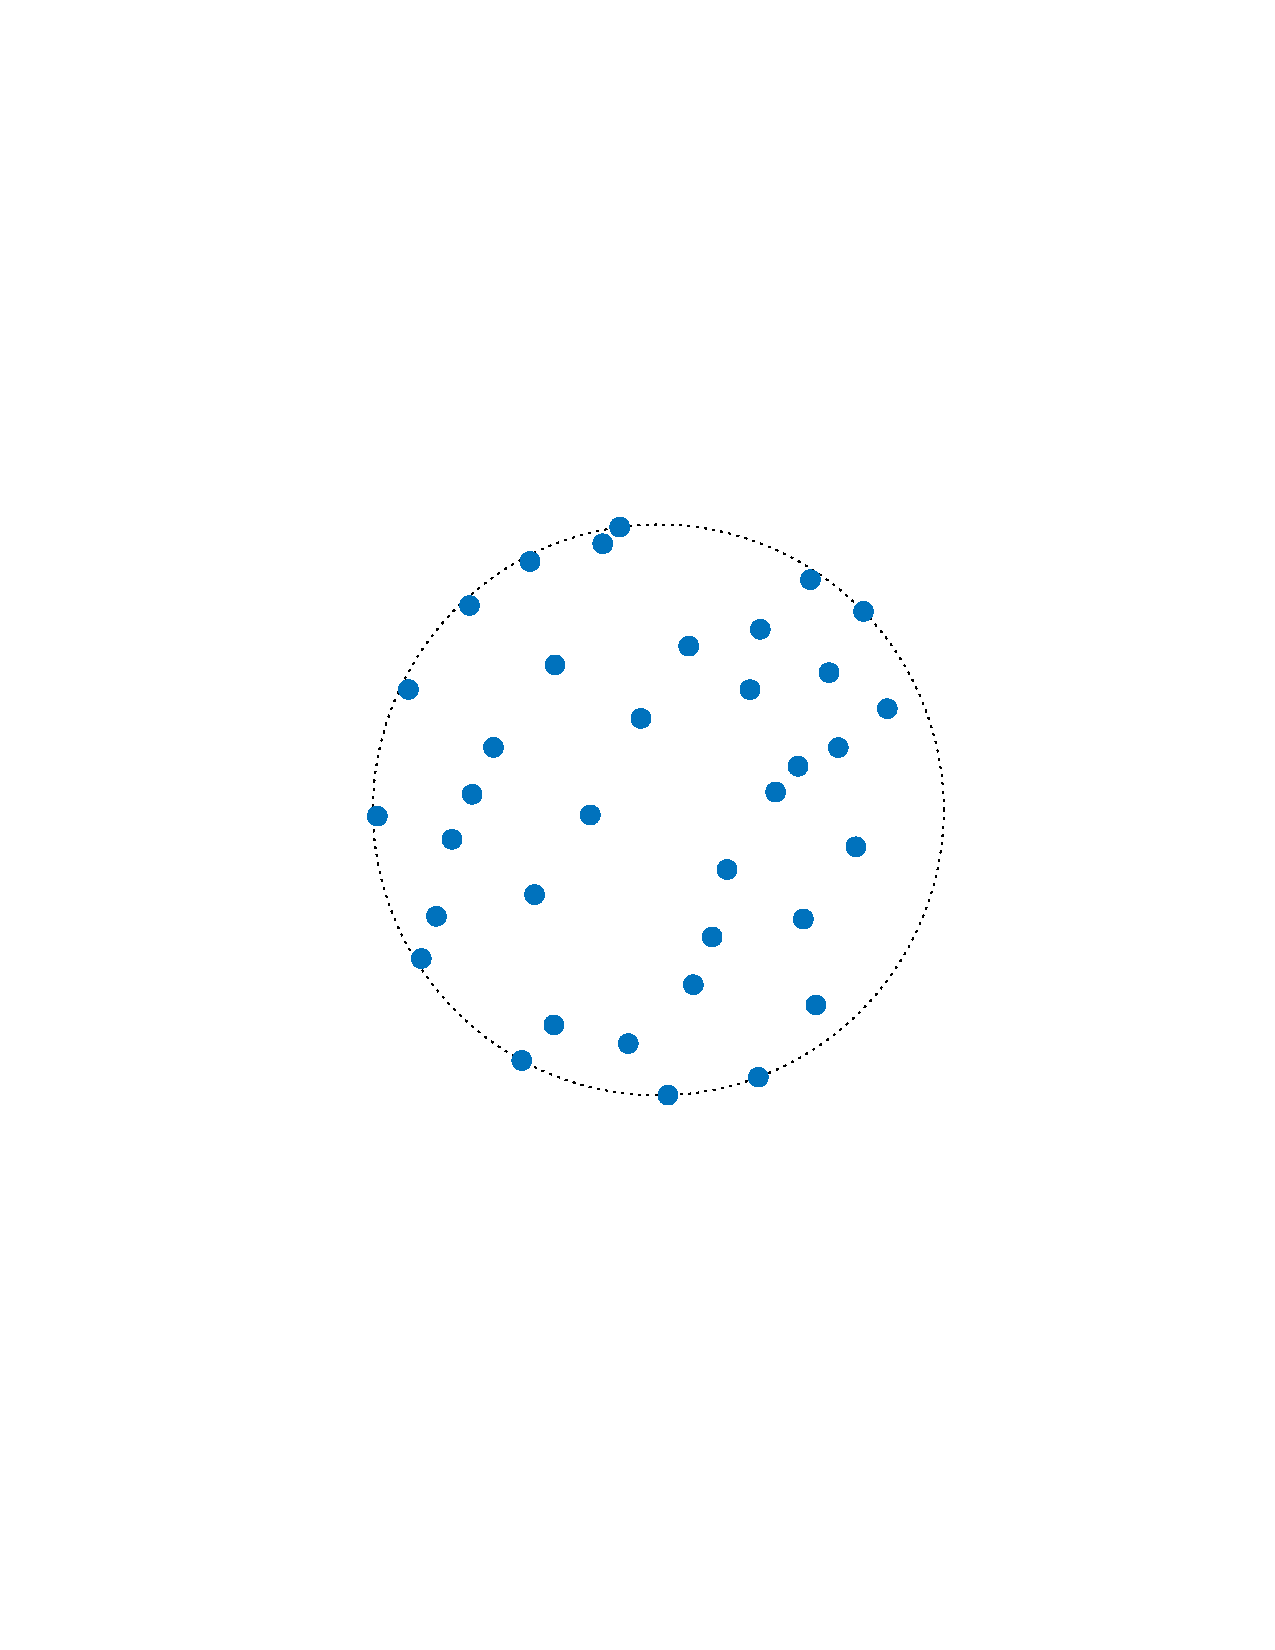
\includegraphics[clip, width=0.3\textwidth, scale=0.025, trim={3cm 8cm 3cm 8cm}]{figures/iea37-opt36-par5.pdf}
	}
	\subfigure[\textit{sub6}]{
		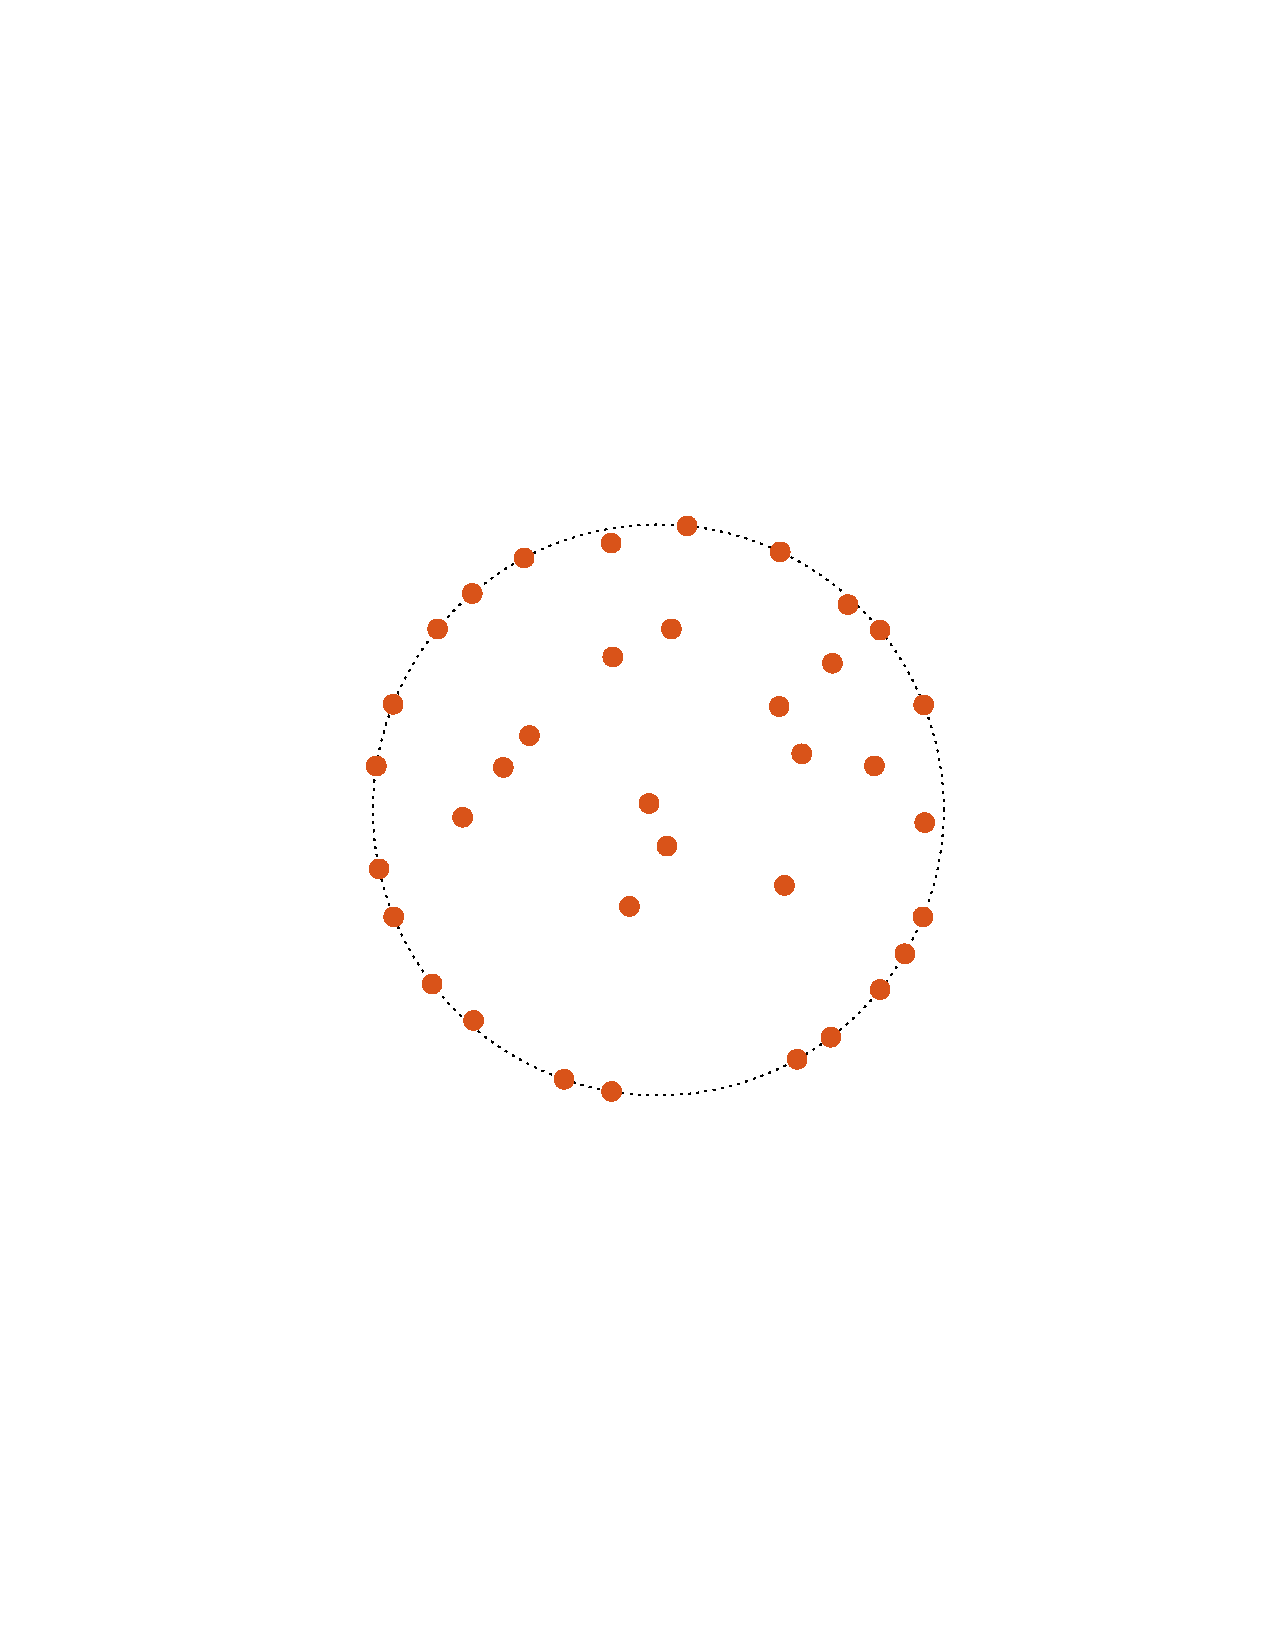
\includegraphics[clip, width=0.3\textwidth, scale=0.025, trim={3cm 8cm 3cm 8cm}]{figures/iea37-opt36-par6.pdf}
	}
	\subfigure[\textit{sub7}]{
		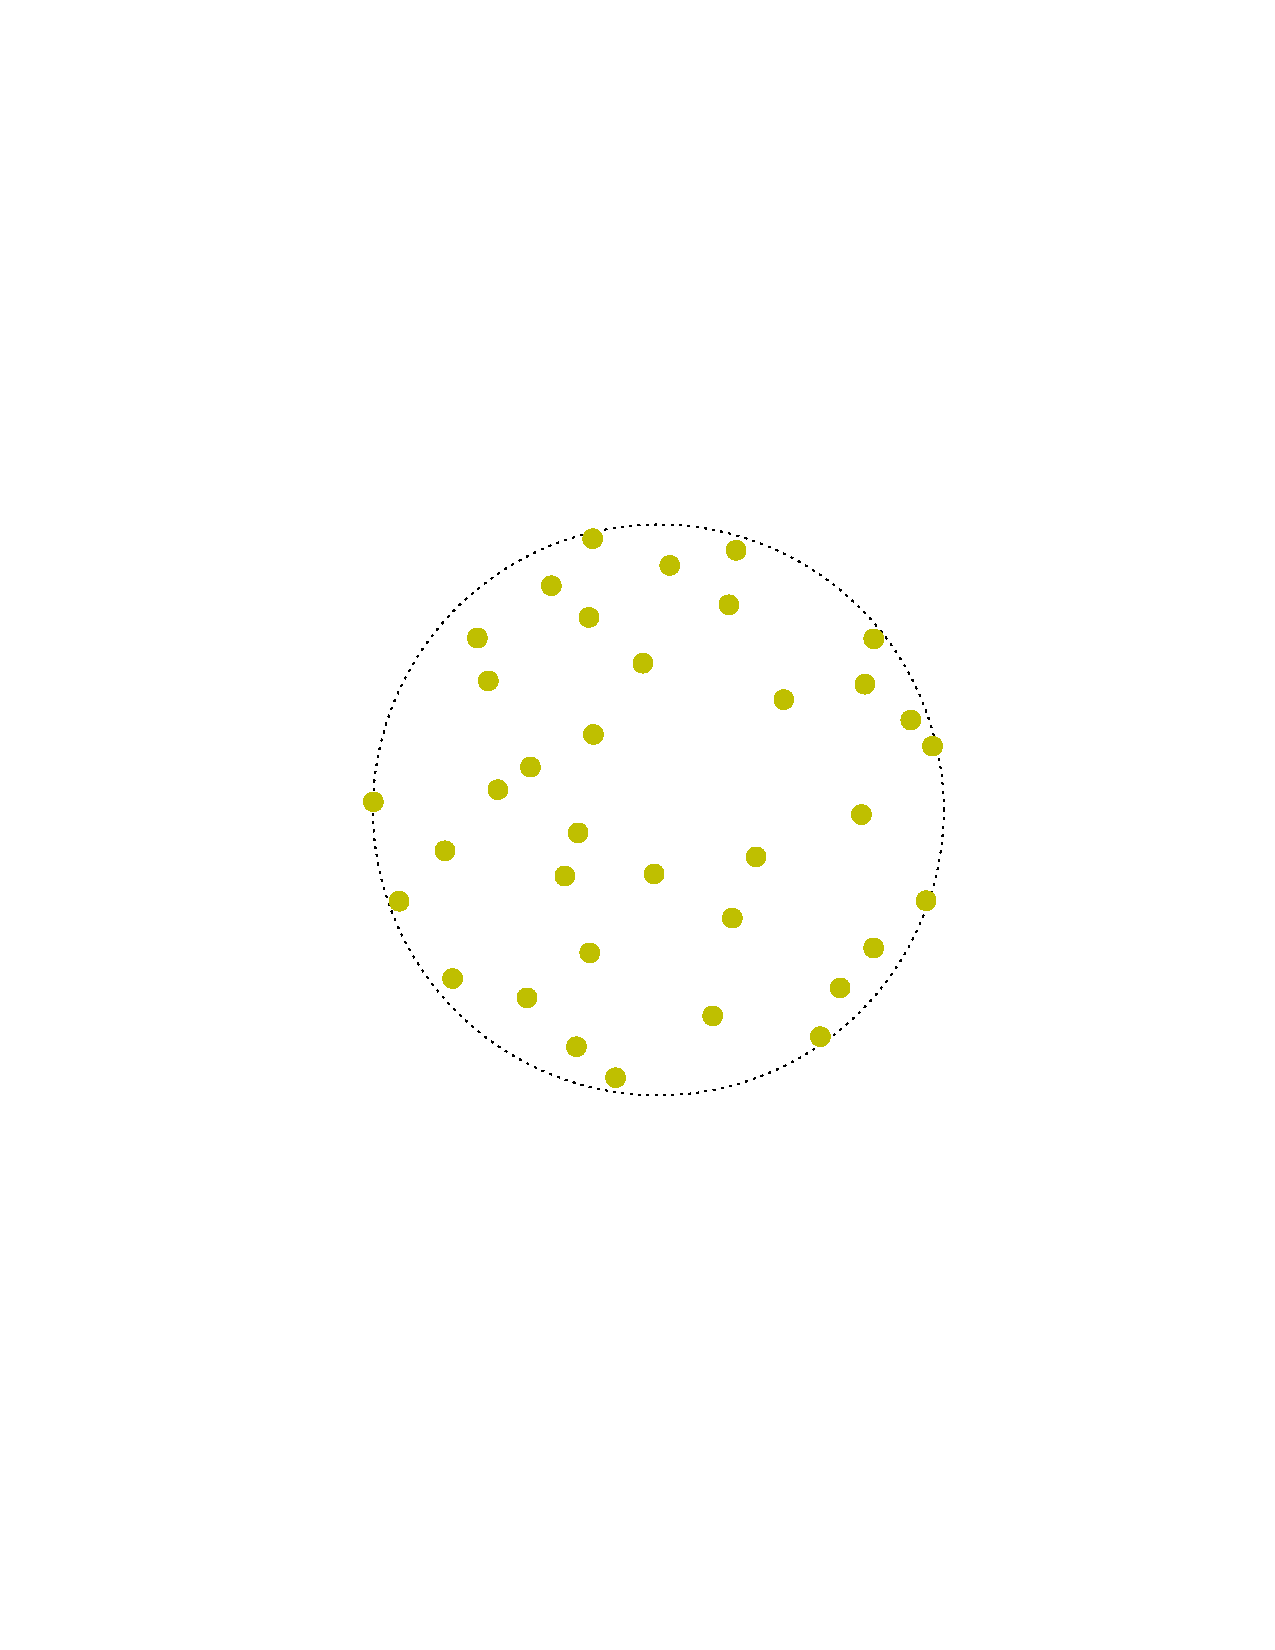
\includegraphics[clip, width=0.3\textwidth,scale=0.025, trim={3cm 8cm 3cm 8cm}]{figures/iea37-opt36-par7.pdf}
	}
	\subfigure[\textit{sub8}]{
		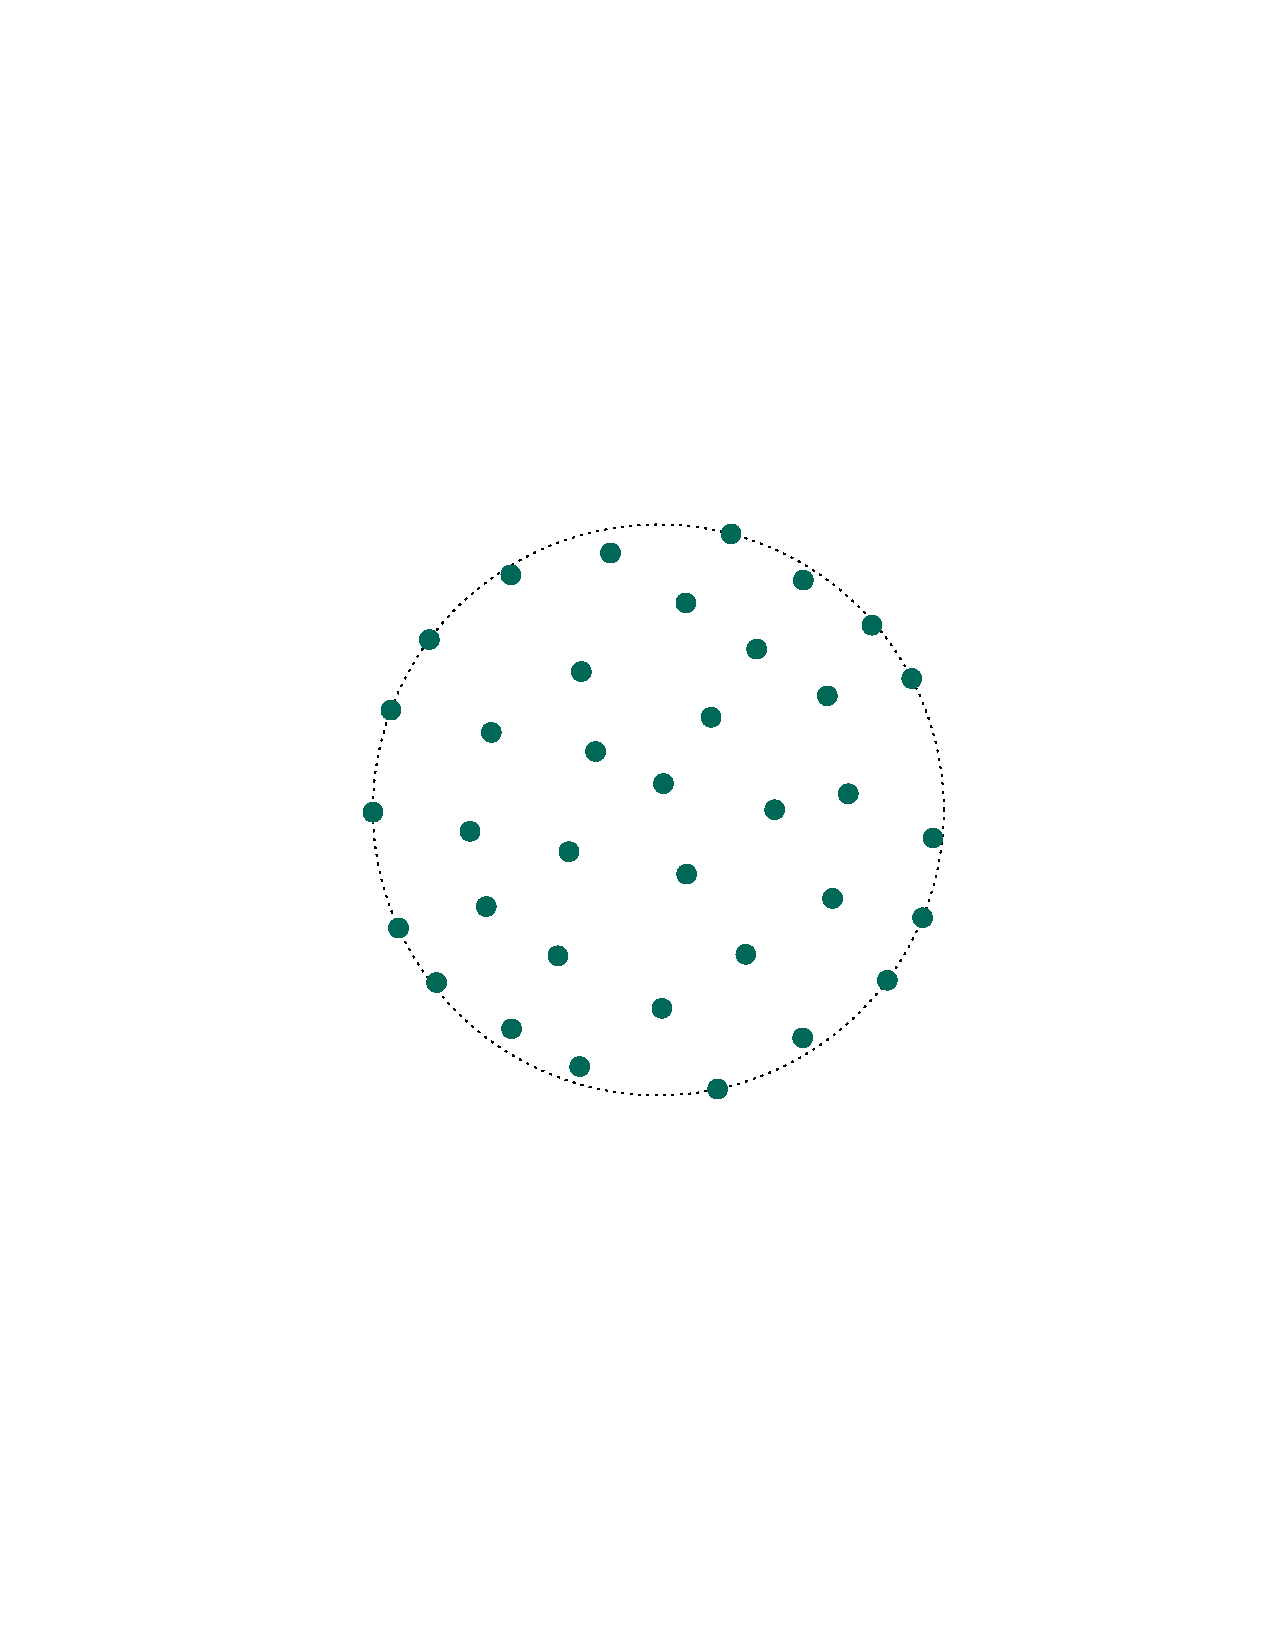
\includegraphics[clip, width=0.3\textwidth,scale=0.025, trim={3cm 8cm 3cm 8cm}]{figures/iea37-opt36-par8.pdf}
	}
	\subfigure[\textit{sub9}]{
		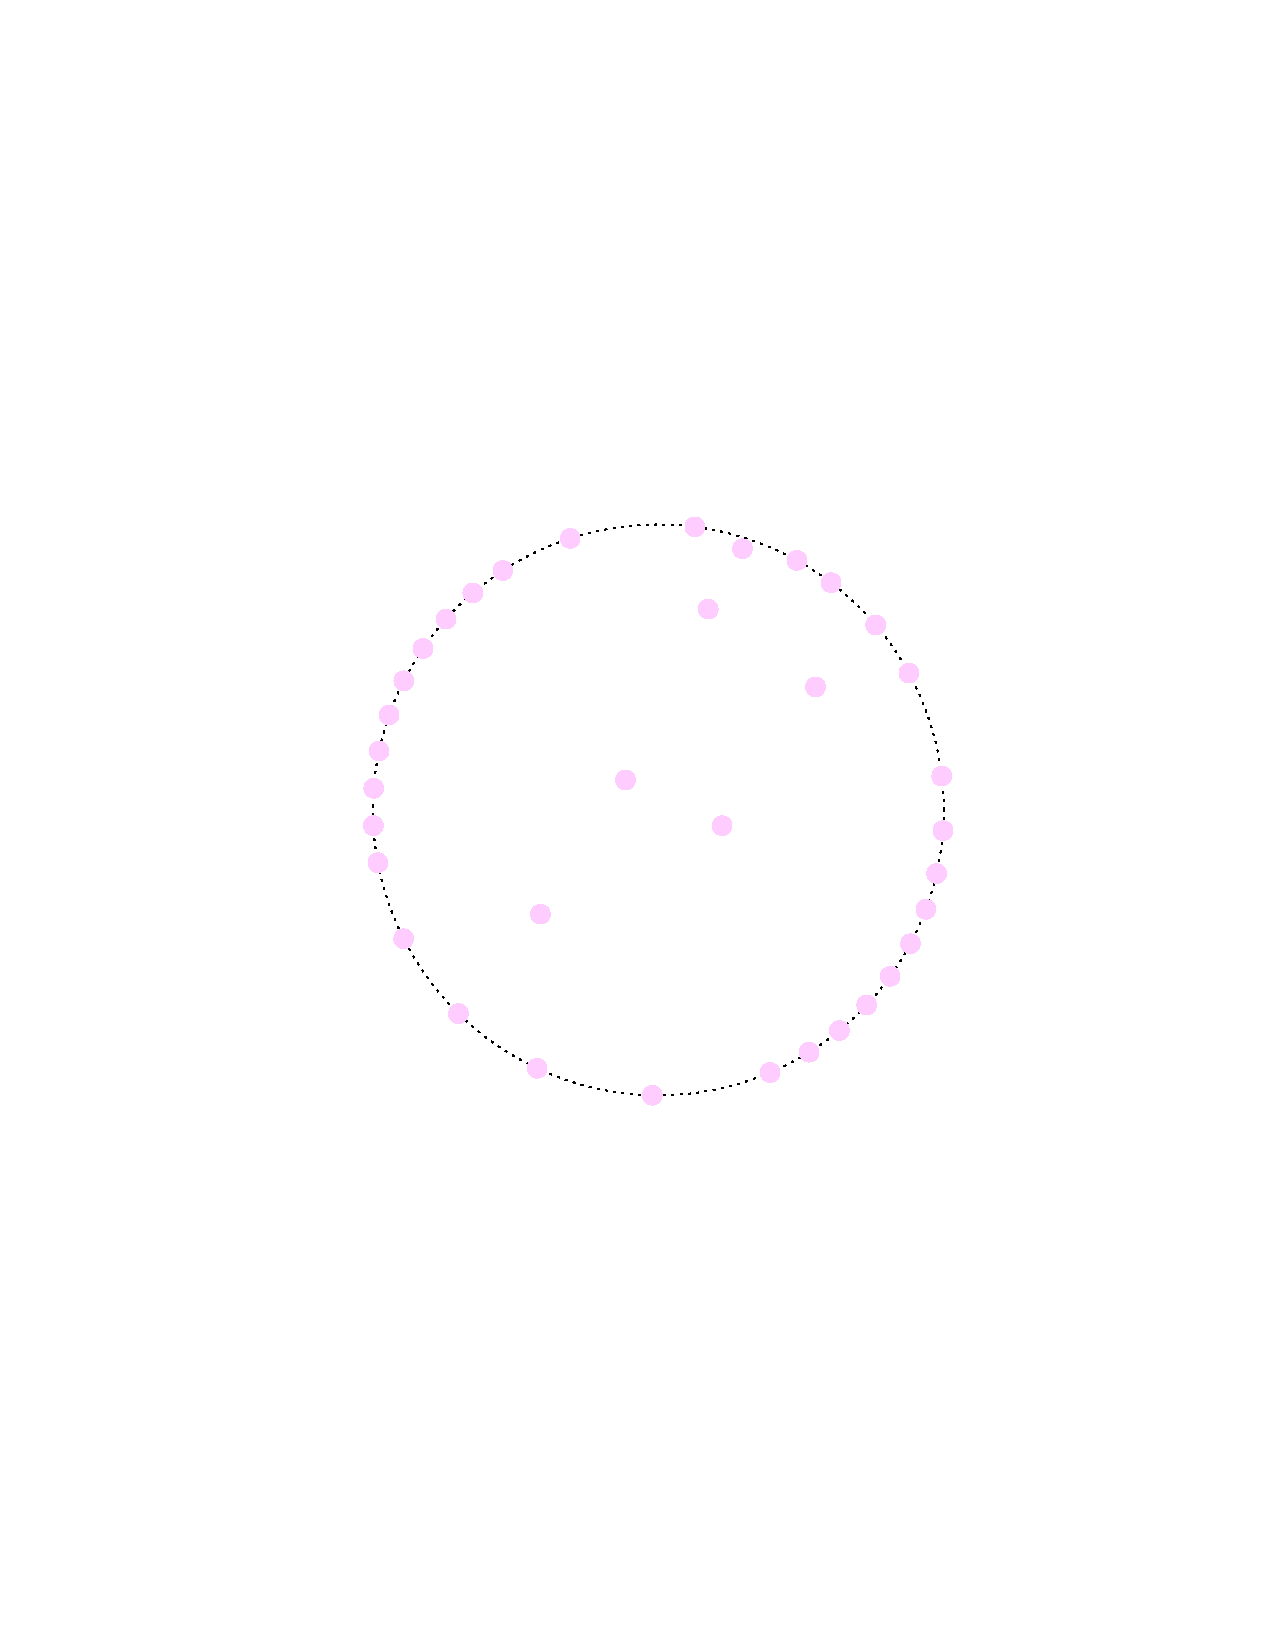
\includegraphics[clip, width=0.3\textwidth, scale=0.025, trim={3cm 8cm 3cm 8cm}]{figures/iea37-opt36-par9.pdf}
	}
	\subfigure[\textit{sub10}]{
		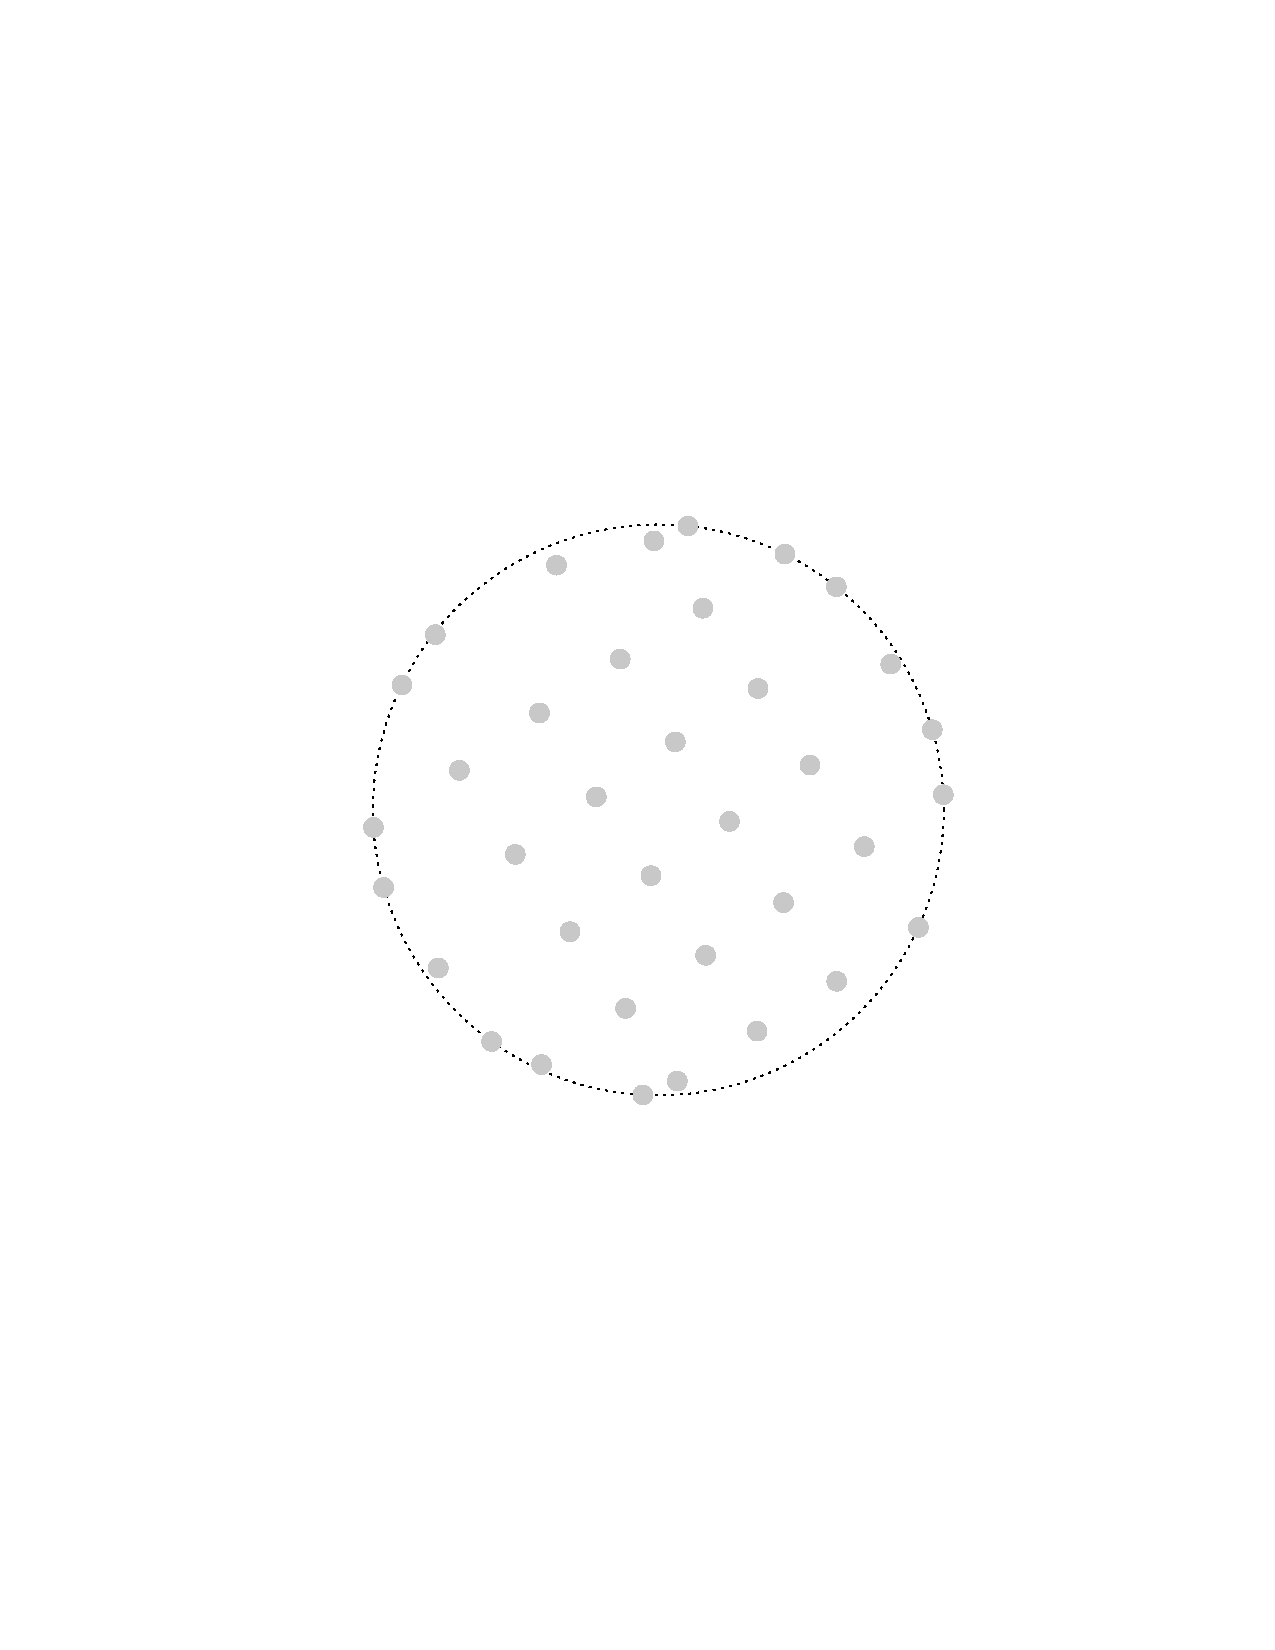
\includegraphics[clip, width=0.3\textwidth, scale=0.025, trim={3cm 8cm 3cm 8cm}]{figures/iea37-opt36-par10.pdf}
    }
    \subfigure[\textit{sub11}]{
		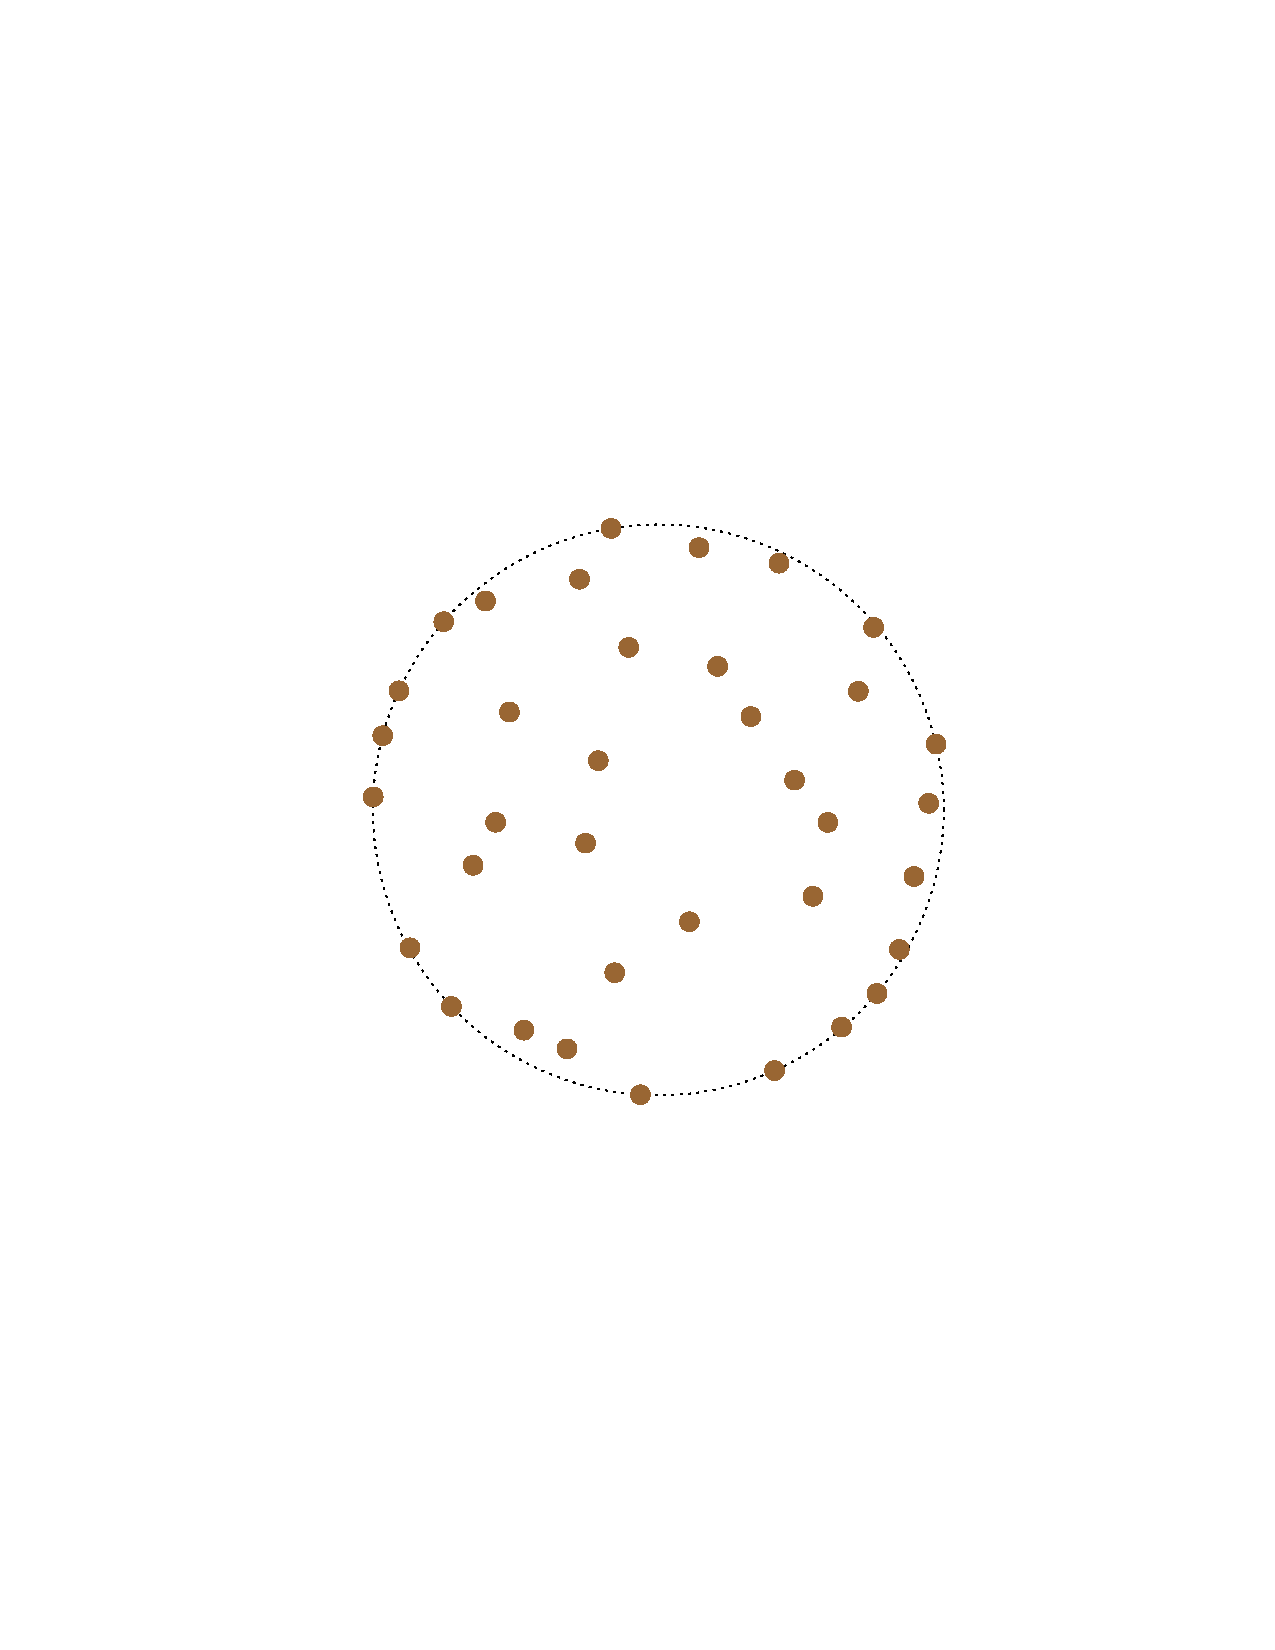
\includegraphics[clip, width=0.3\textwidth, scale=0.025, trim={3cm 8cm 3cm 8cm}]{figures/iea37-opt36-par11.pdf}
	}
	\subfigure[\textit{sub12}]{
		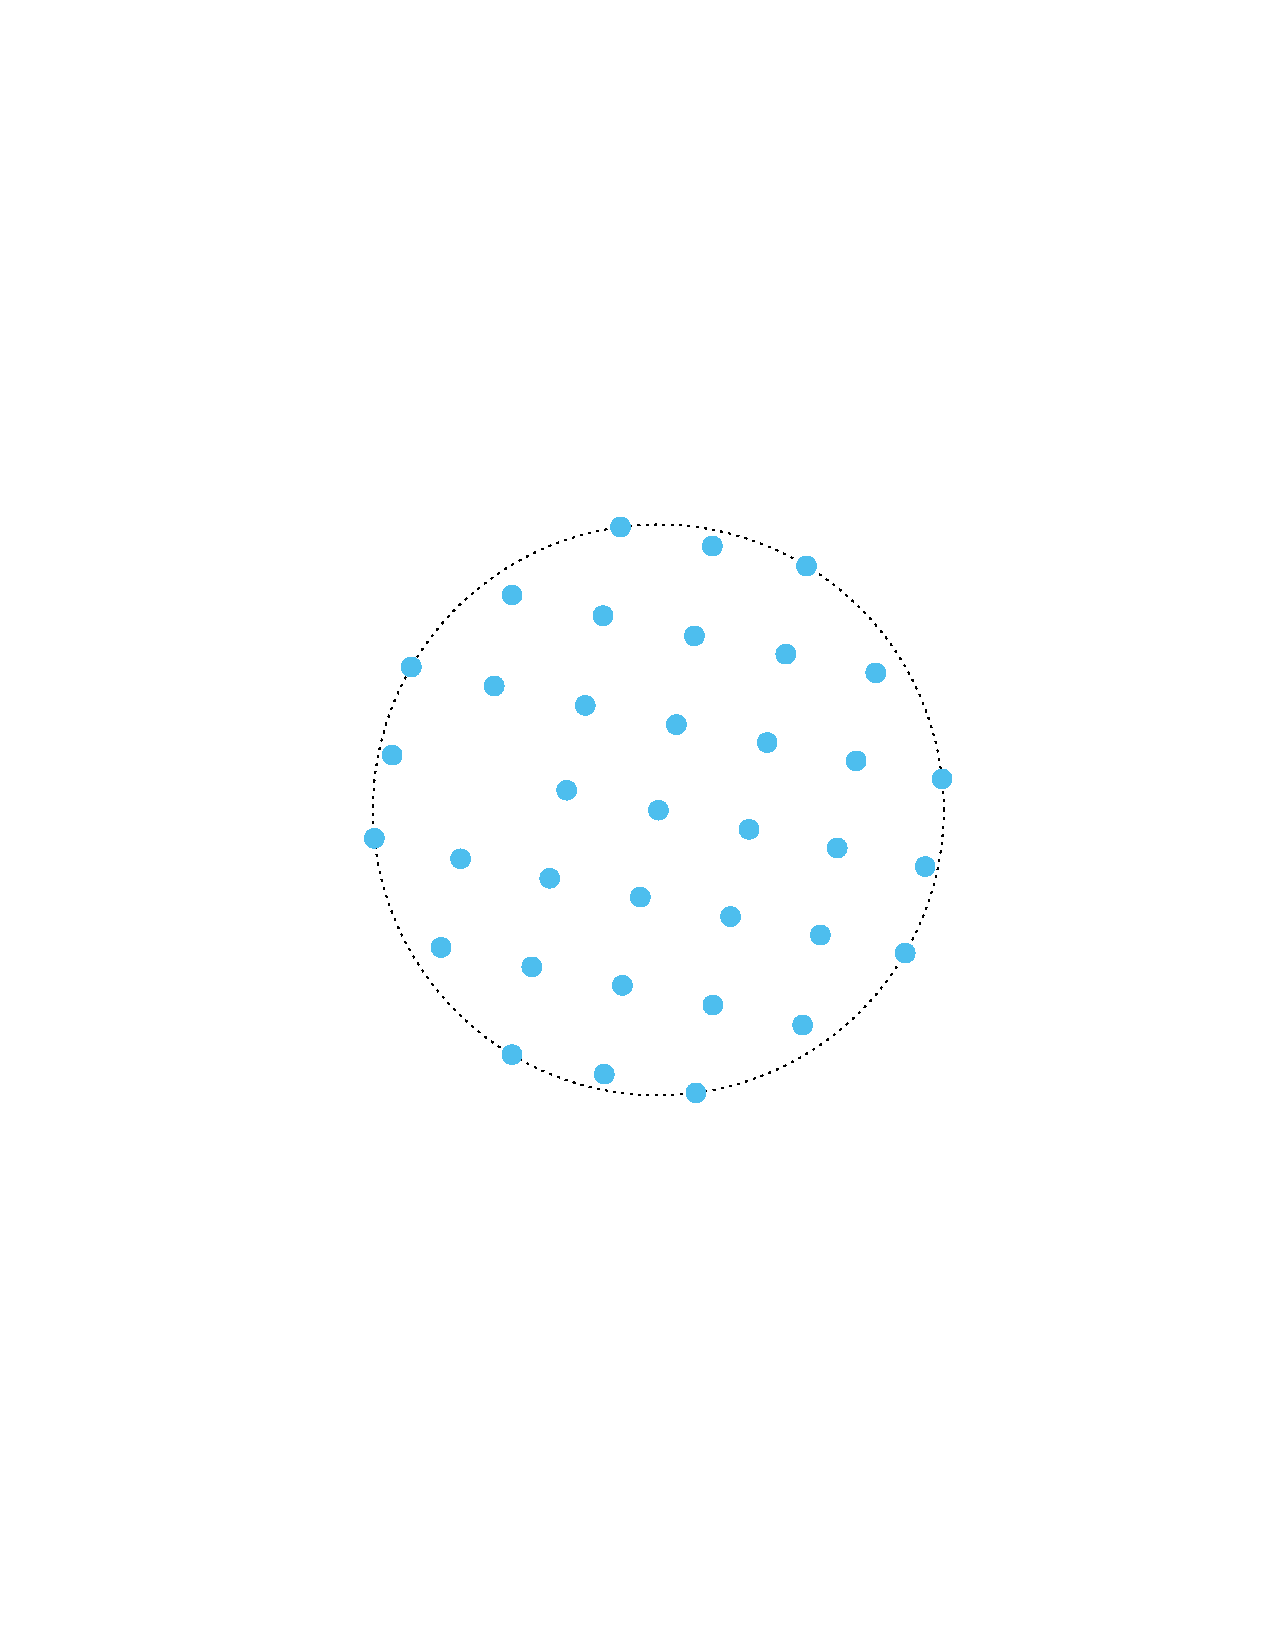
\includegraphics[clip, width=0.3\textwidth, scale=0.025, trim={3cm 8cm 3cm 8cm}]{figures/iea37-opt36-par12.pdf}
	}
	\caption{Case study 1: optimized wind farm layouts with 36 wind turbines.}
	\label{fig:36turbs}
\end{figure}

\begin{figure}[htbp!]
	\centering
	\subfigure[\textit{sub1}]{
		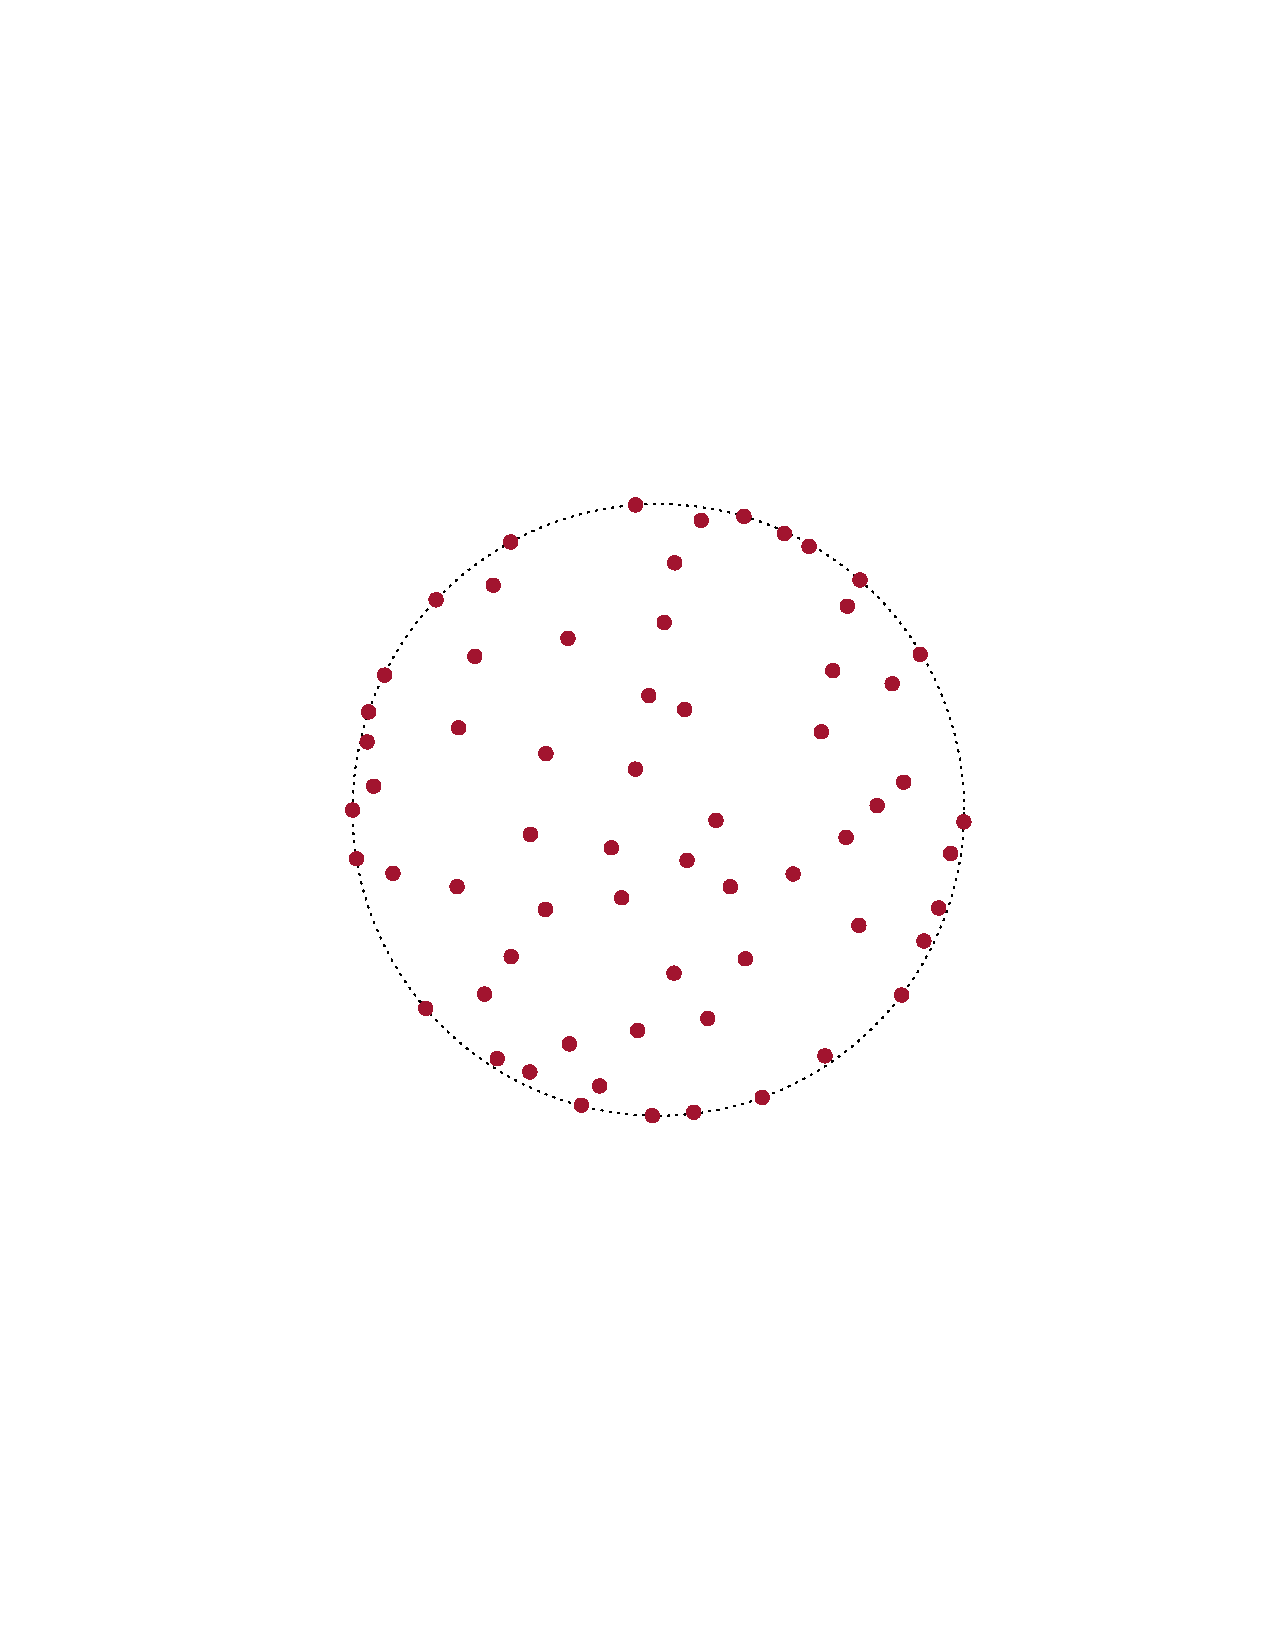
\includegraphics[clip, width=0.3\textwidth, scale=0.025, trim={3cm 8cm 3cm 8cm}]{figures/iea37-opt64-par1.pdf}
	}
	\subfigure[\textit{sub2}]{
		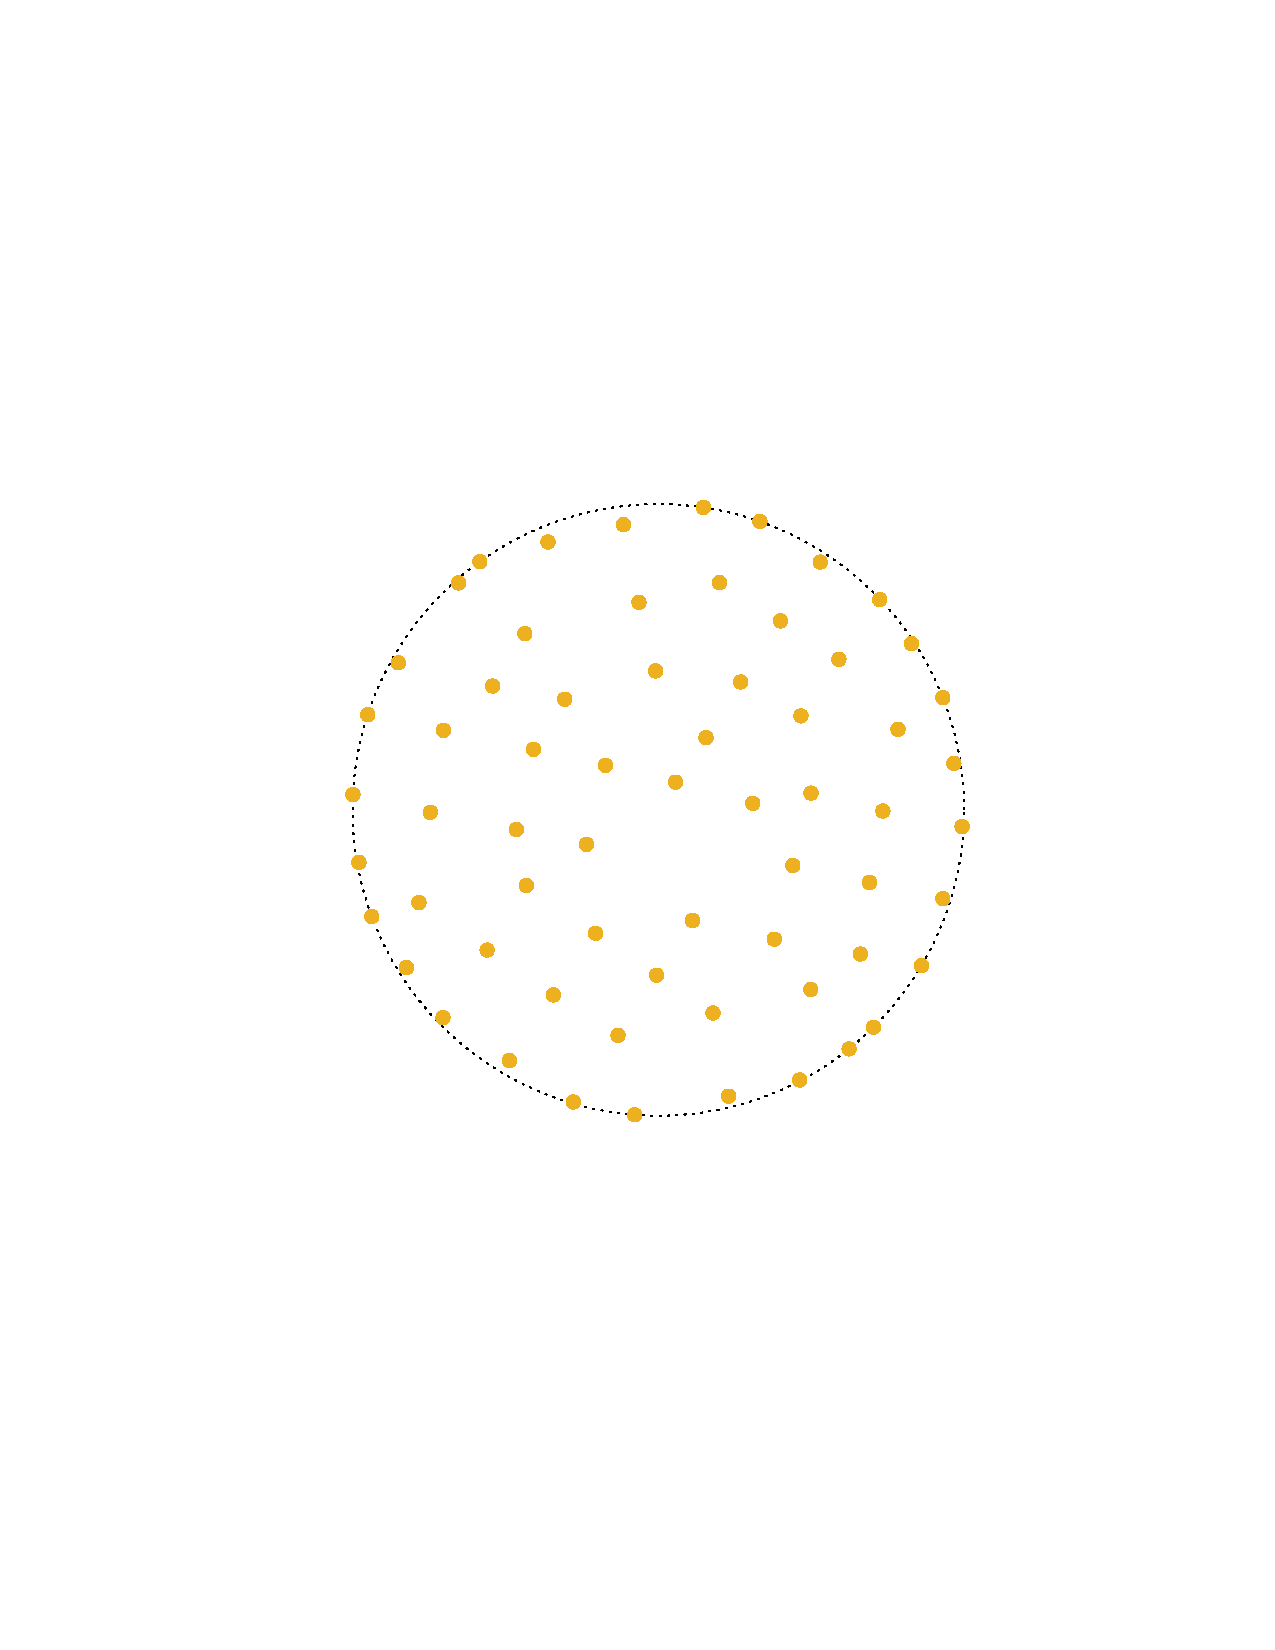
\includegraphics[clip, width=0.3\textwidth,scale=0.025, trim={3cm 8cm 3cm 8cm}]{figures/iea37-opt64-par2.pdf}
	}
	\subfigure[\textit{sub3}]{
		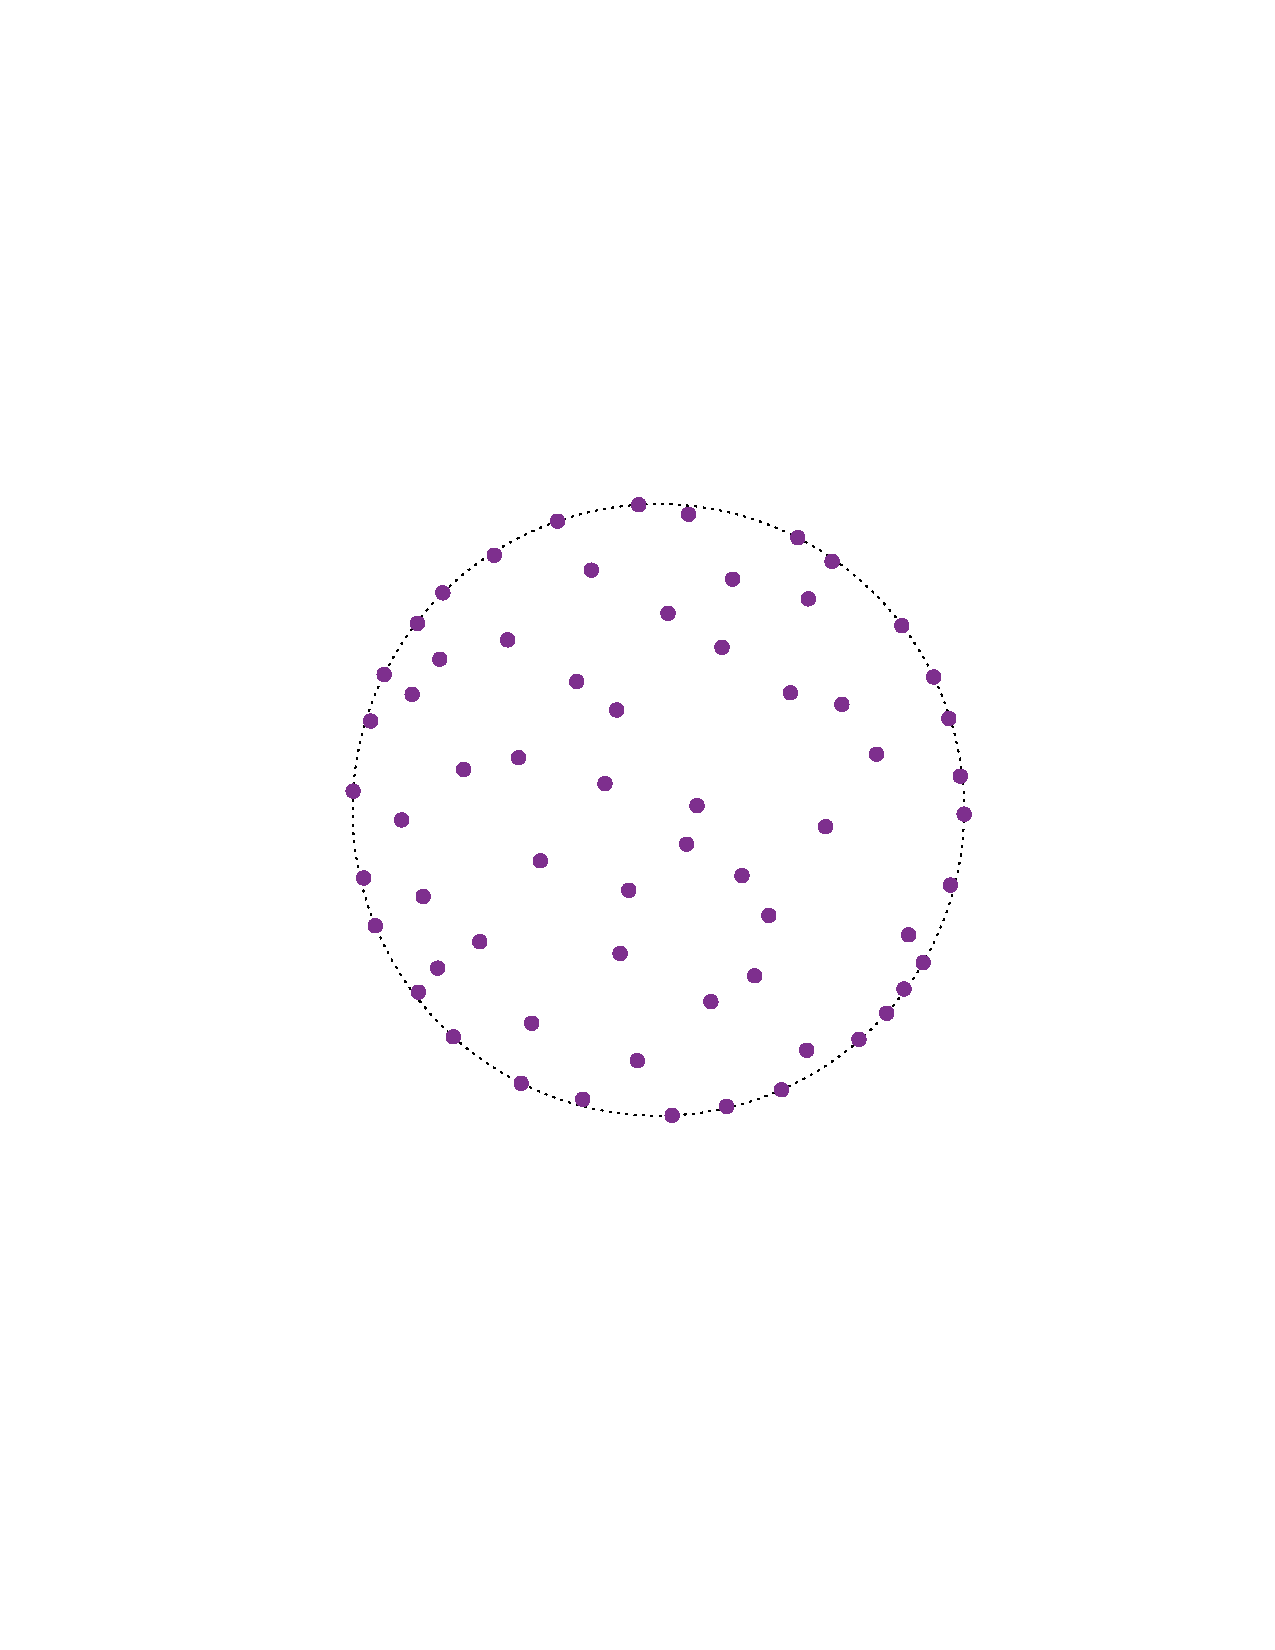
\includegraphics[clip, width=0.3\textwidth,scale=0.025, trim={3cm 8cm 3cm 8cm}]{figures/iea37-opt64-par3.pdf}
	}
	\subfigure[\textit{sub4}]{
		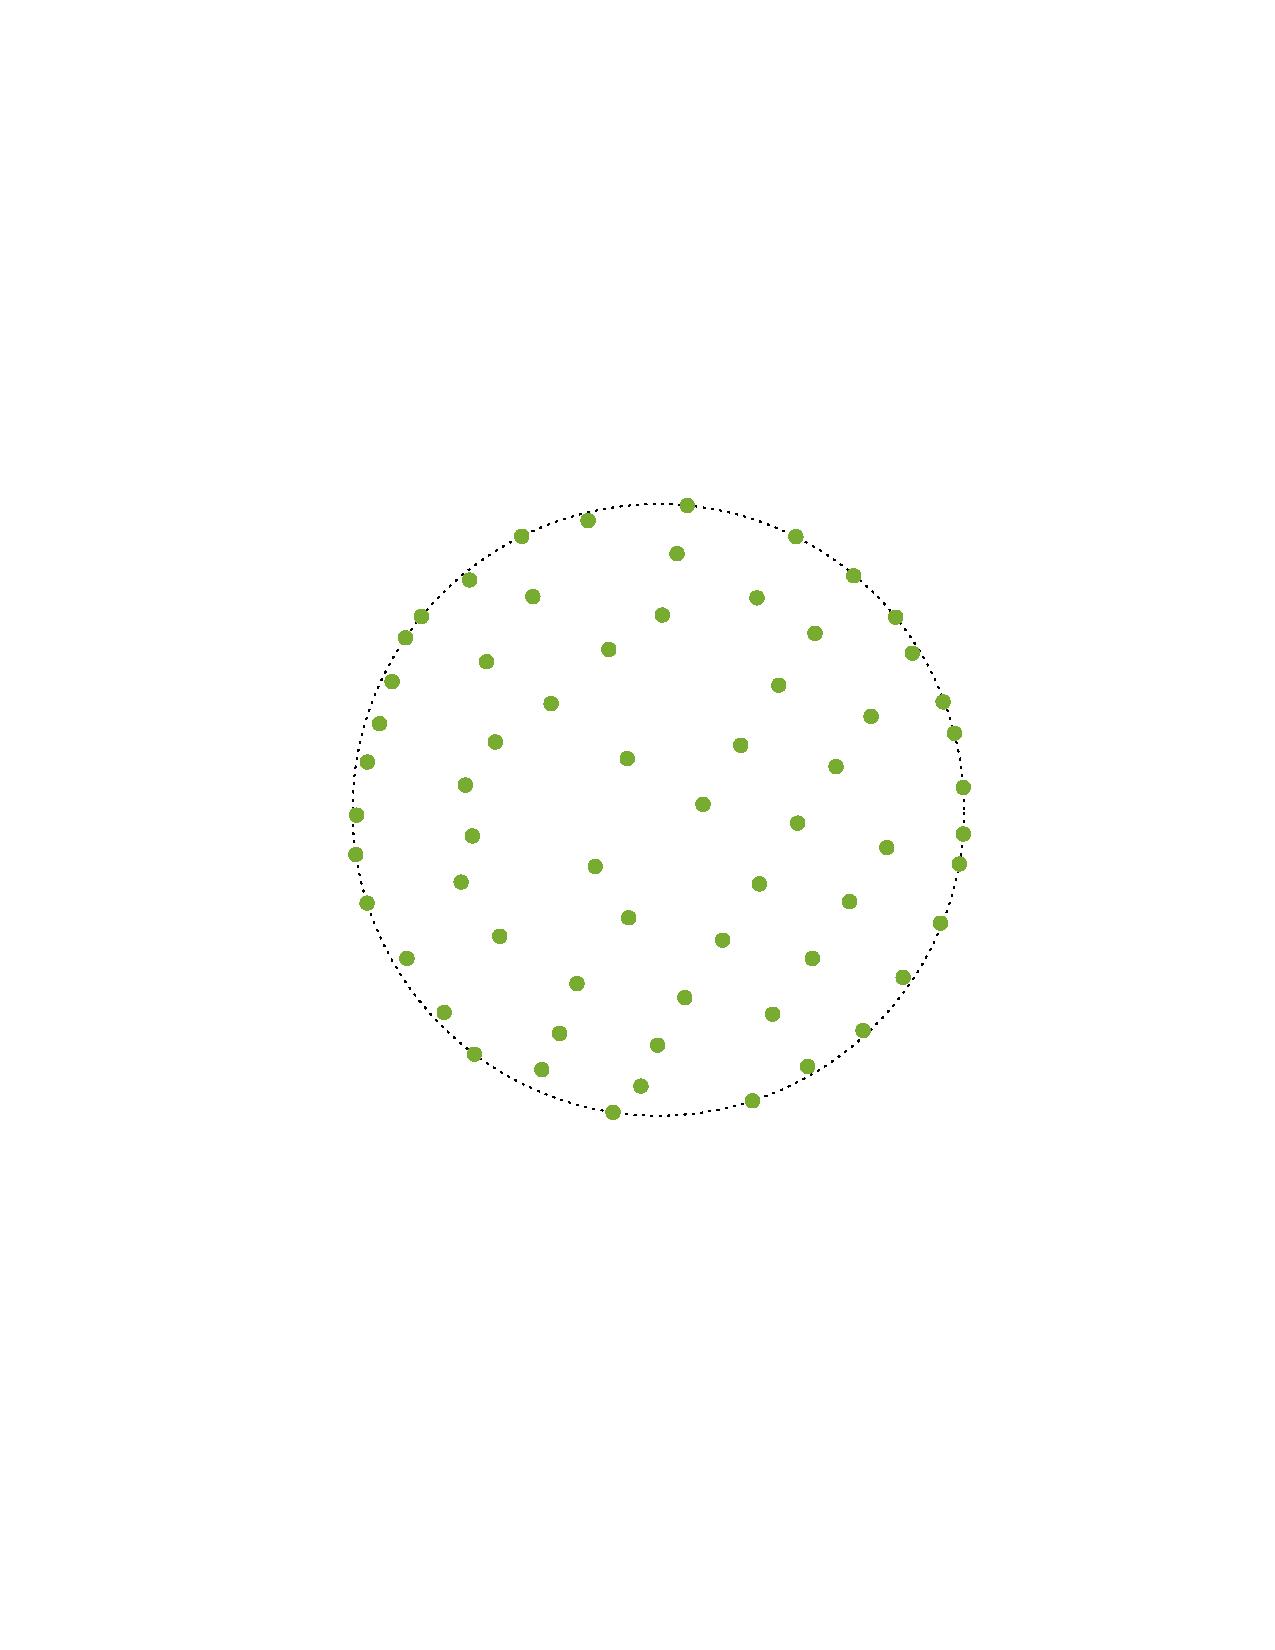
\includegraphics[clip, width=0.3\textwidth, scale=0.025, trim={3cm 8cm 3cm 8cm}]{figures/iea37-opt64-par4.pdf}
	}
	\subfigure[\textit{sub5}]{
		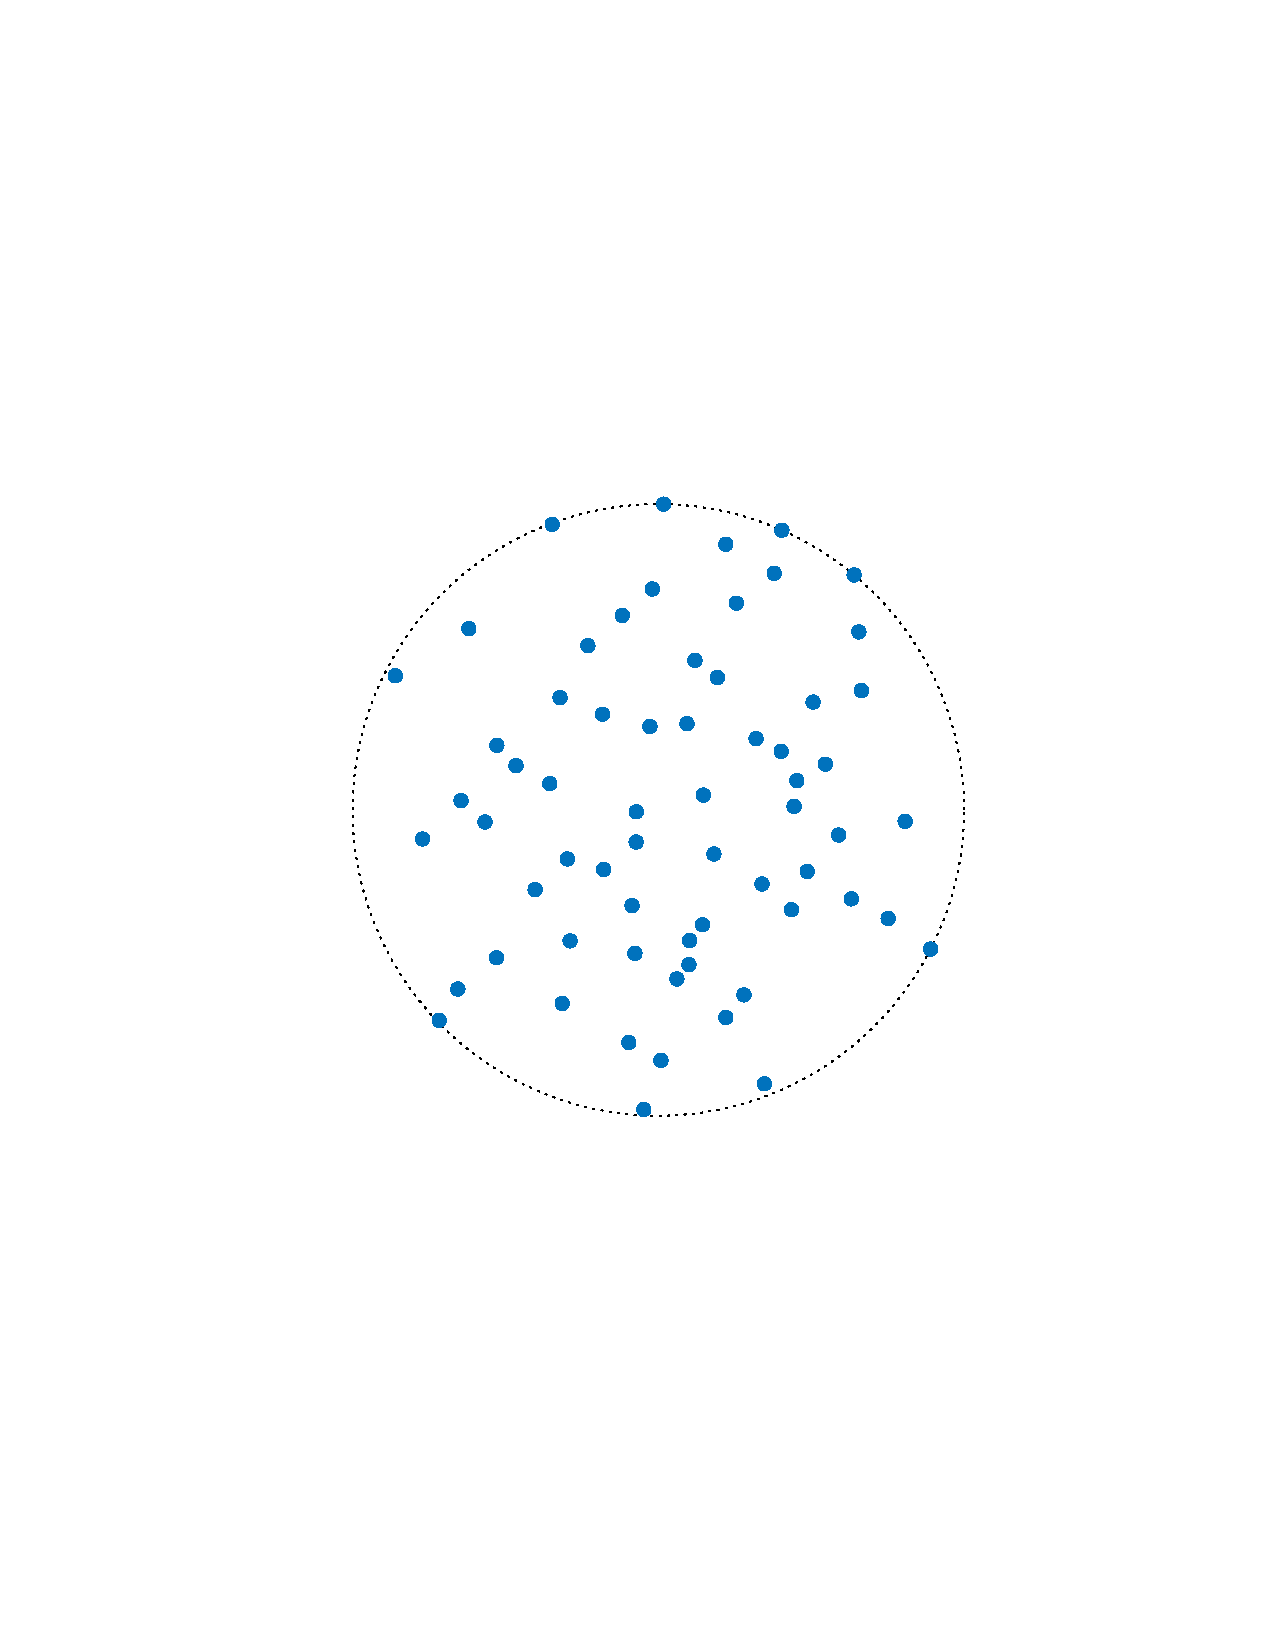
\includegraphics[clip, width=0.3\textwidth, scale=0.025, trim={3cm 8cm 3cm 8cm}]{figures/iea37-opt64-par5.pdf}
	}
	\subfigure[\textit{sub6}]{
		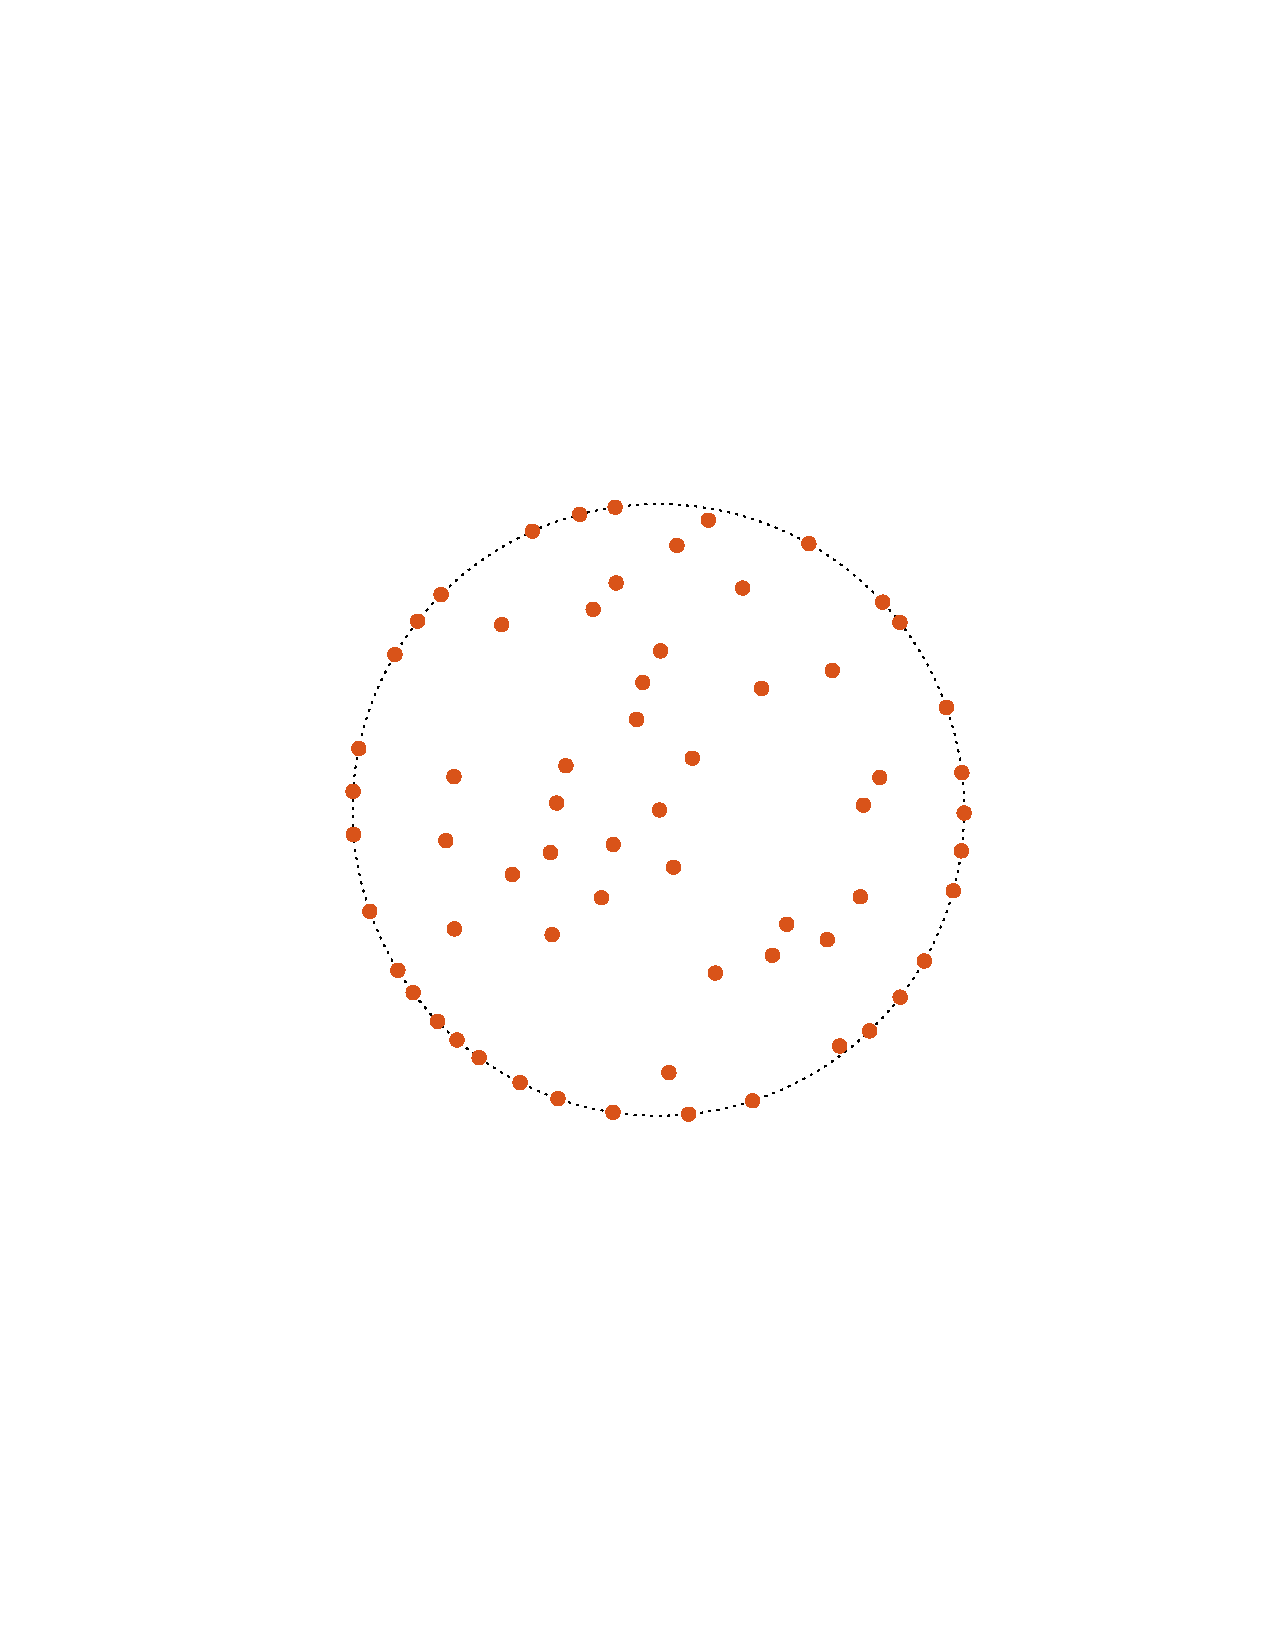
\includegraphics[clip, width=0.3\textwidth, scale=0.025, trim={3cm 8cm 3cm 8cm}]{figures/iea37-opt64-par6.pdf}
	}
	\subfigure[\textit{sub7}]{
		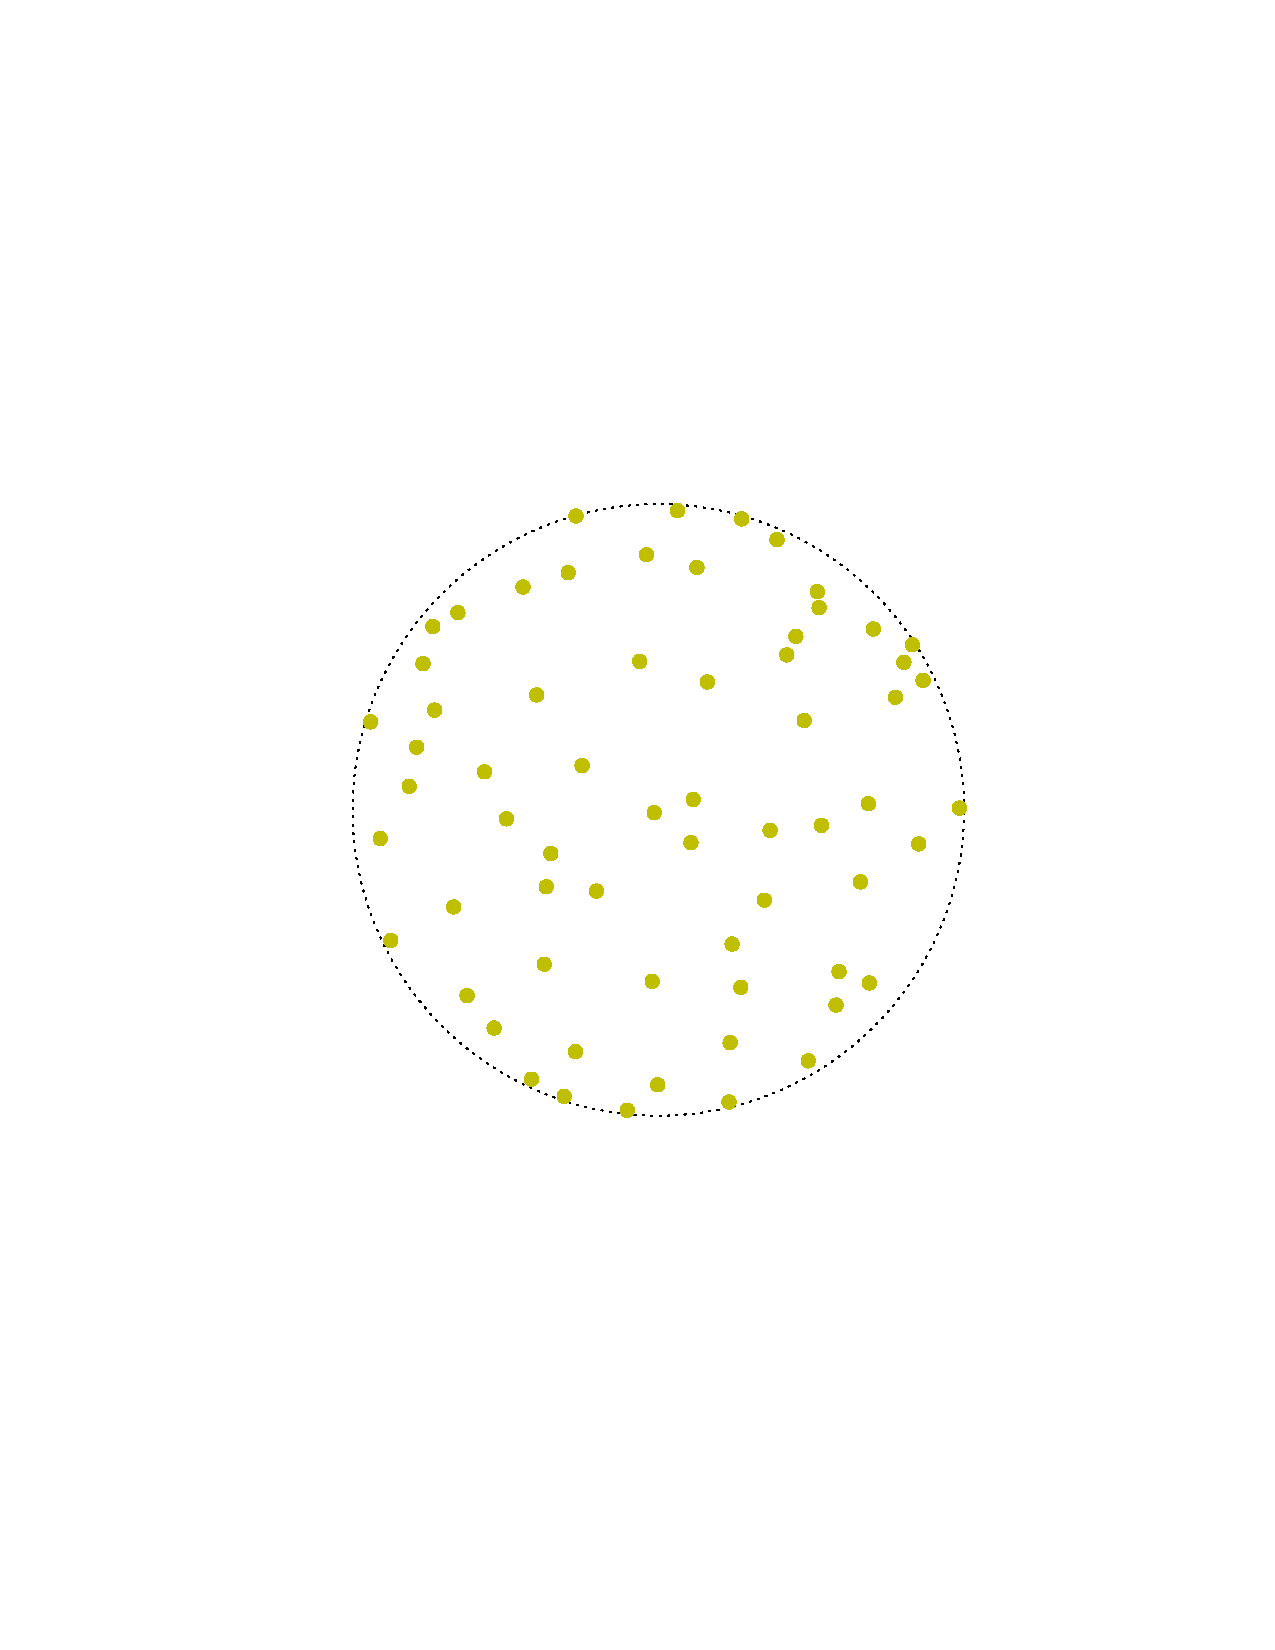
\includegraphics[clip, width=0.3\textwidth,scale=0.025, trim={3cm 8cm 3cm 8cm}]{figures/iea37-opt64-par7.pdf}
	}
	\subfigure[\textit{sub8}]{
		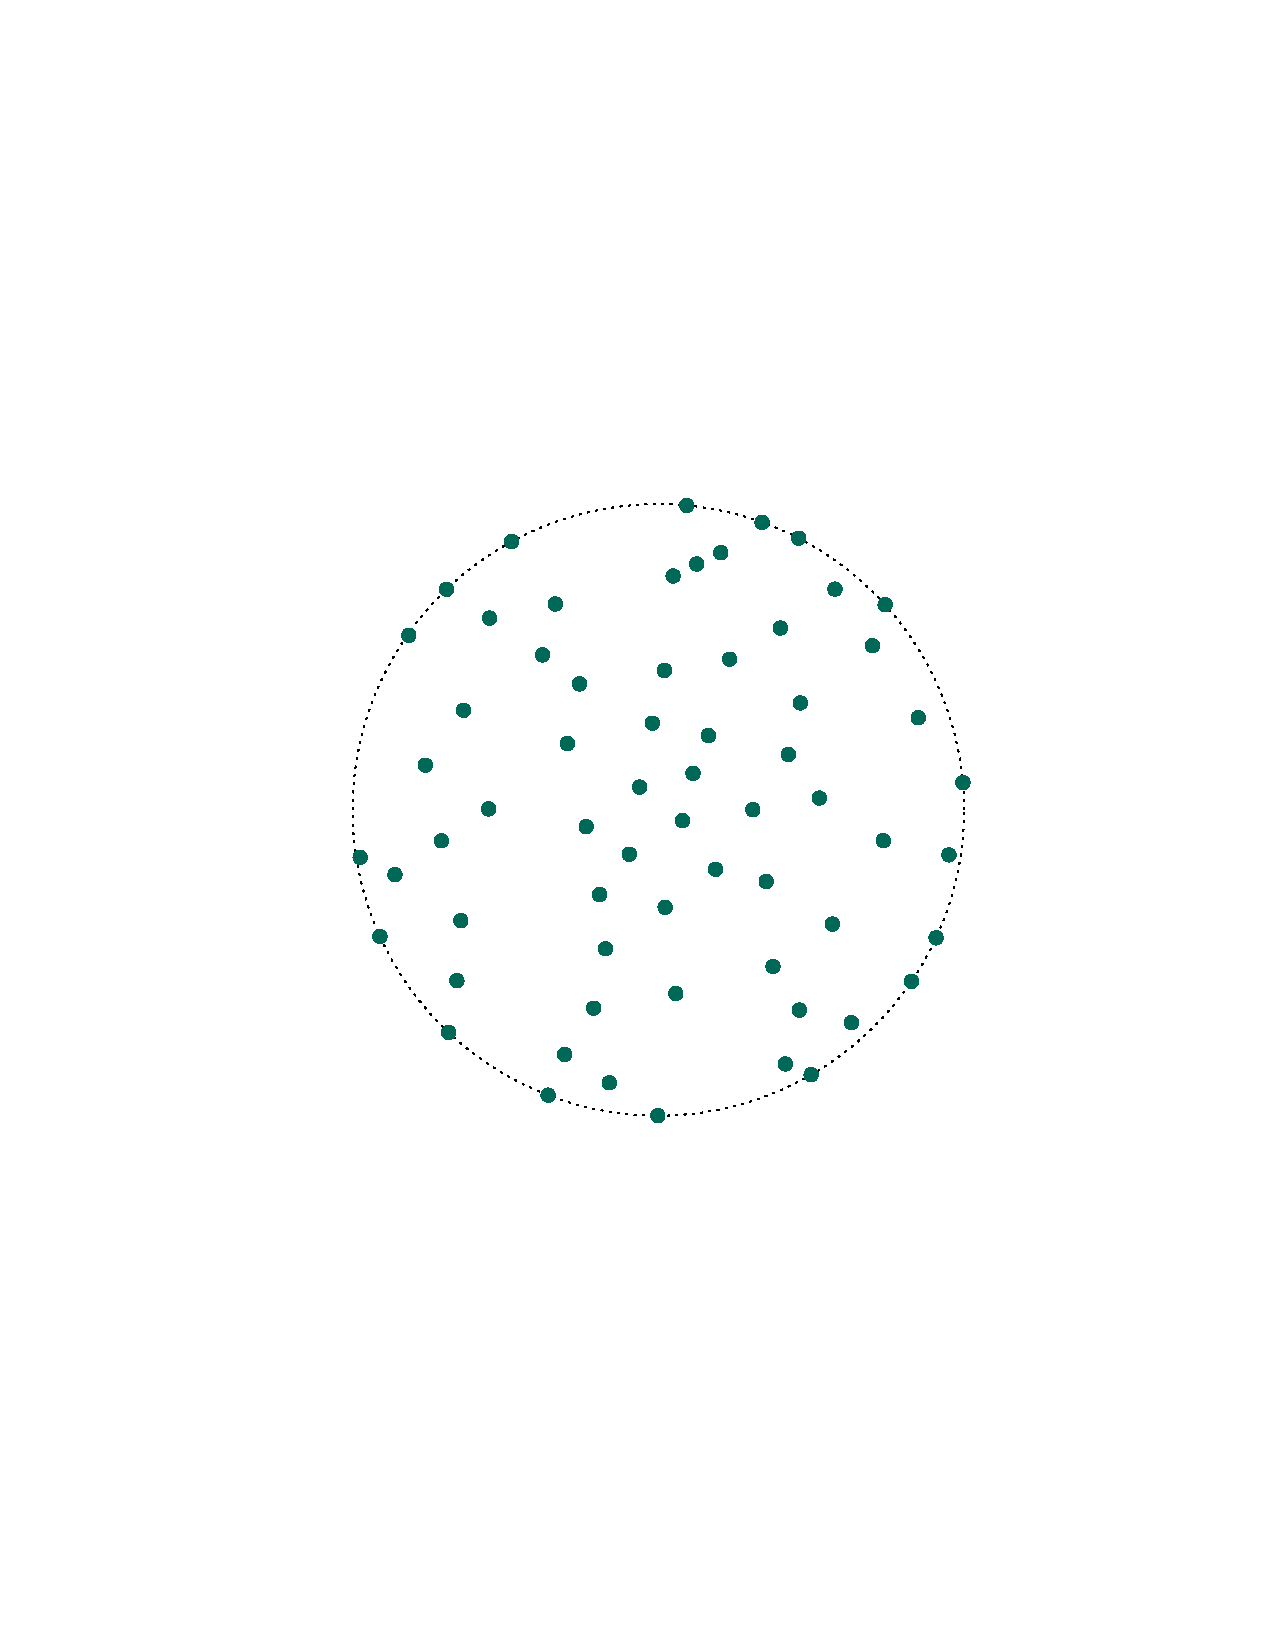
\includegraphics[clip, width=0.3\textwidth,scale=0.025, trim={3cm 8cm 3cm 8cm}]{figures/iea37-opt64-par8.pdf}
	}
	\subfigure[\textit{sub9}]{
		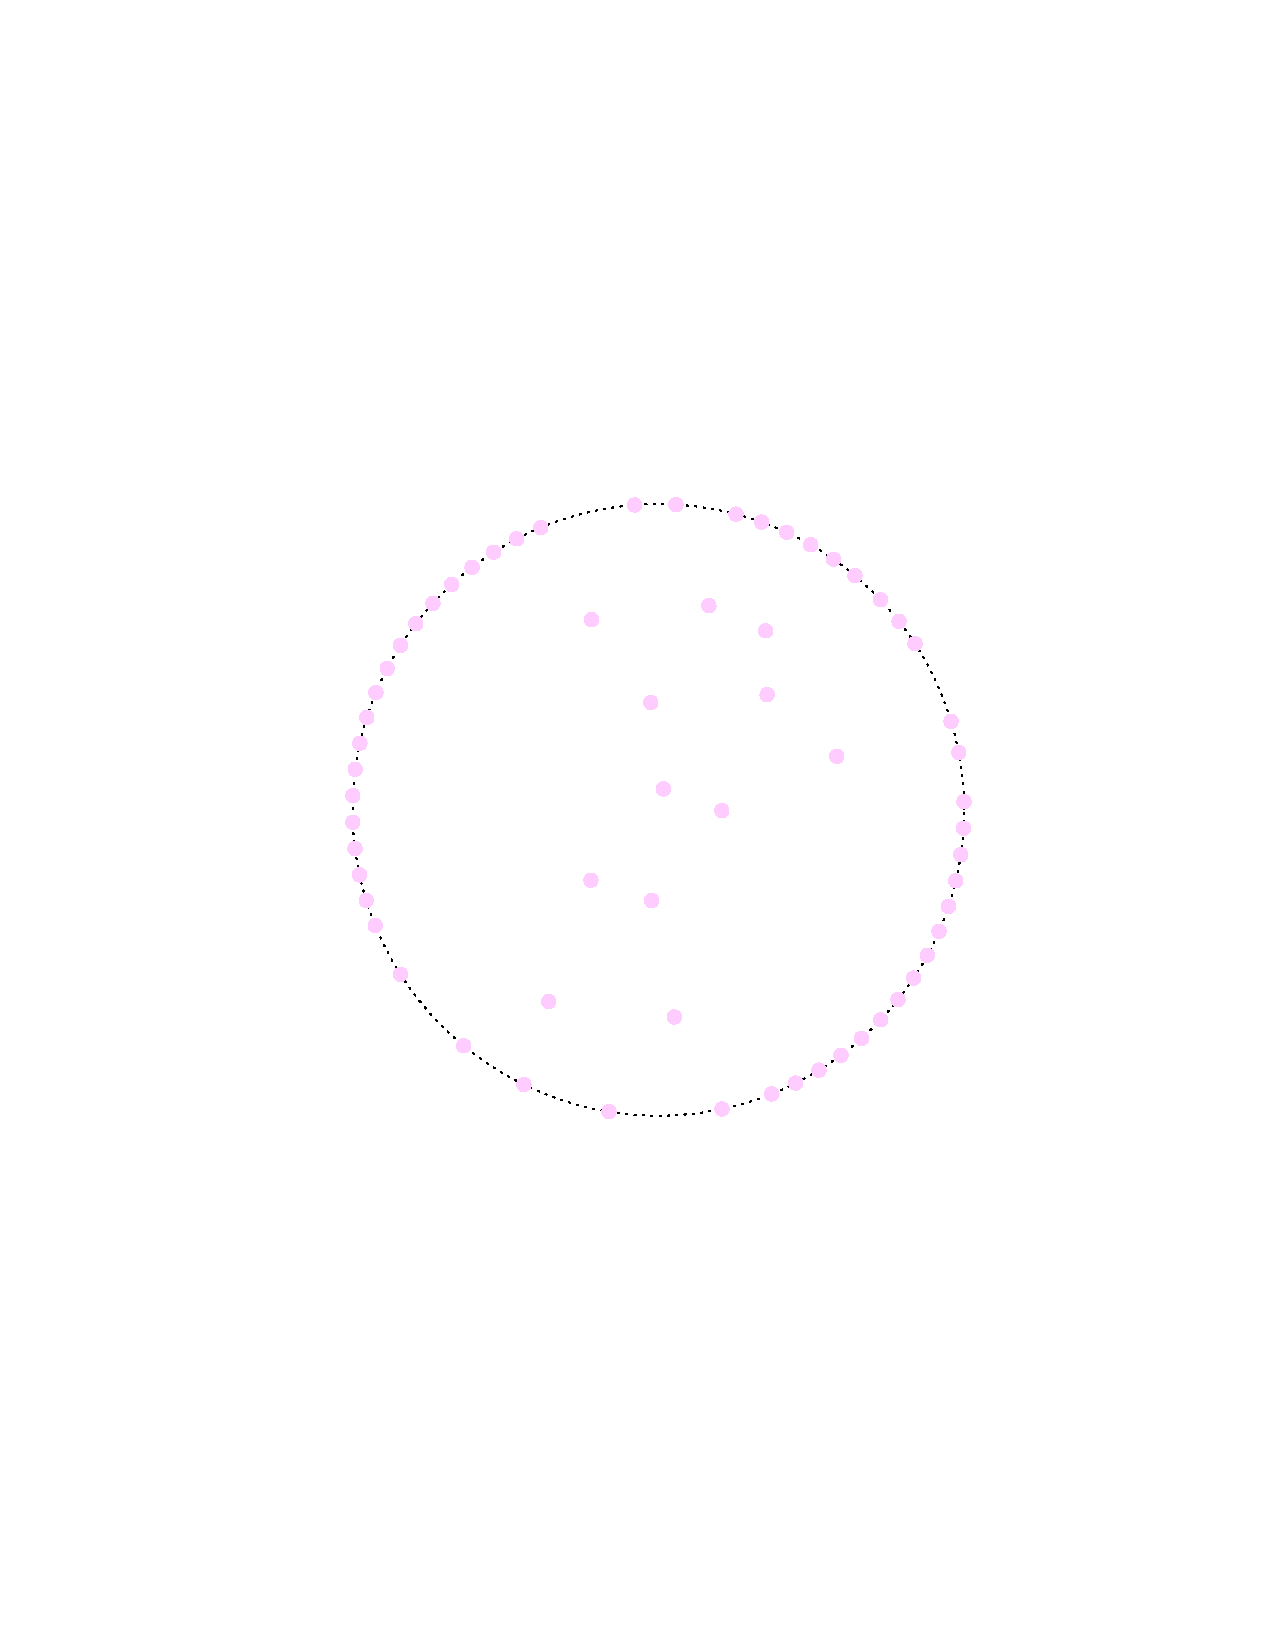
\includegraphics[clip, width=0.3\textwidth, scale=0.025, trim={3cm 8cm 3cm 8cm}]{figures/iea37-opt64-par9.pdf}
	}
	\subfigure[\textit{sub10}]{
		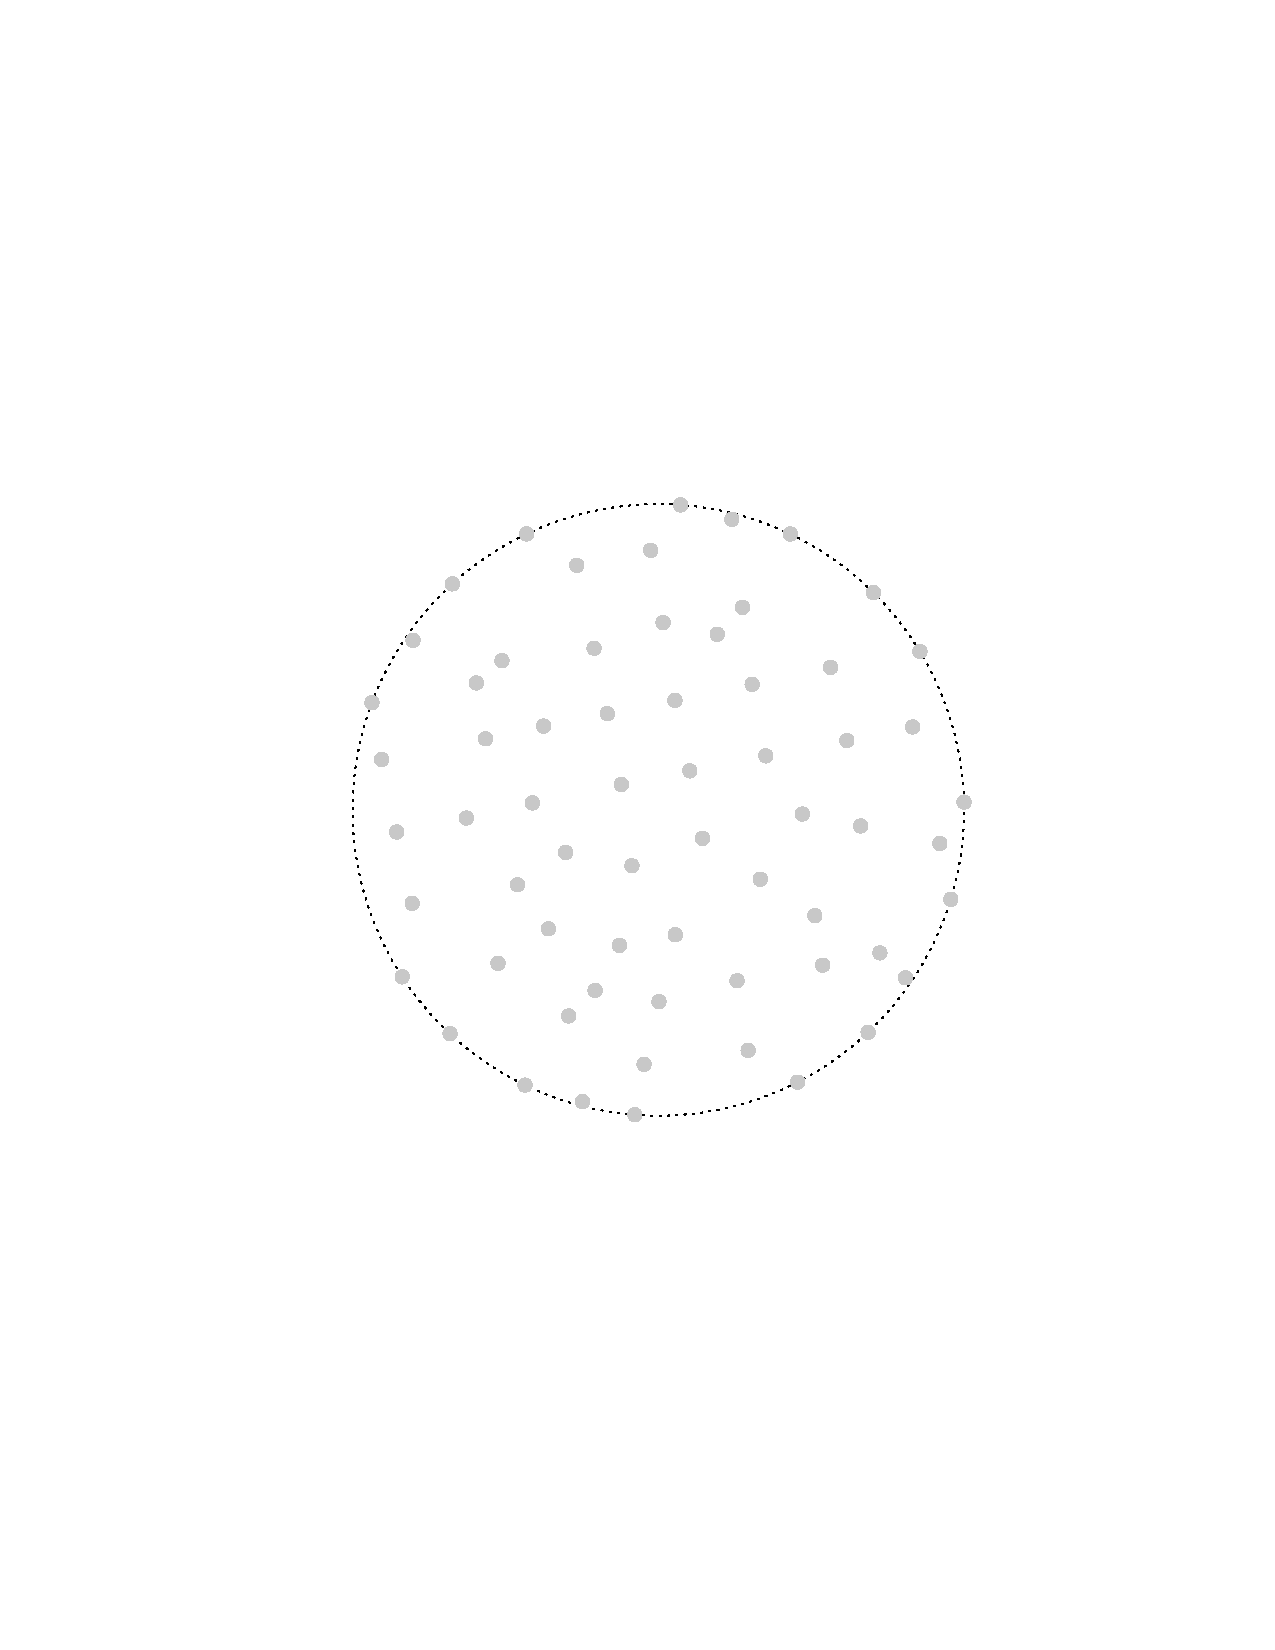
\includegraphics[clip, width=0.3\textwidth, scale=0.025, trim={3cm 8cm 3cm 8cm}]{figures/iea37-opt64-par10.pdf}
    }
    \subfigure[\textit{sub11}]{
		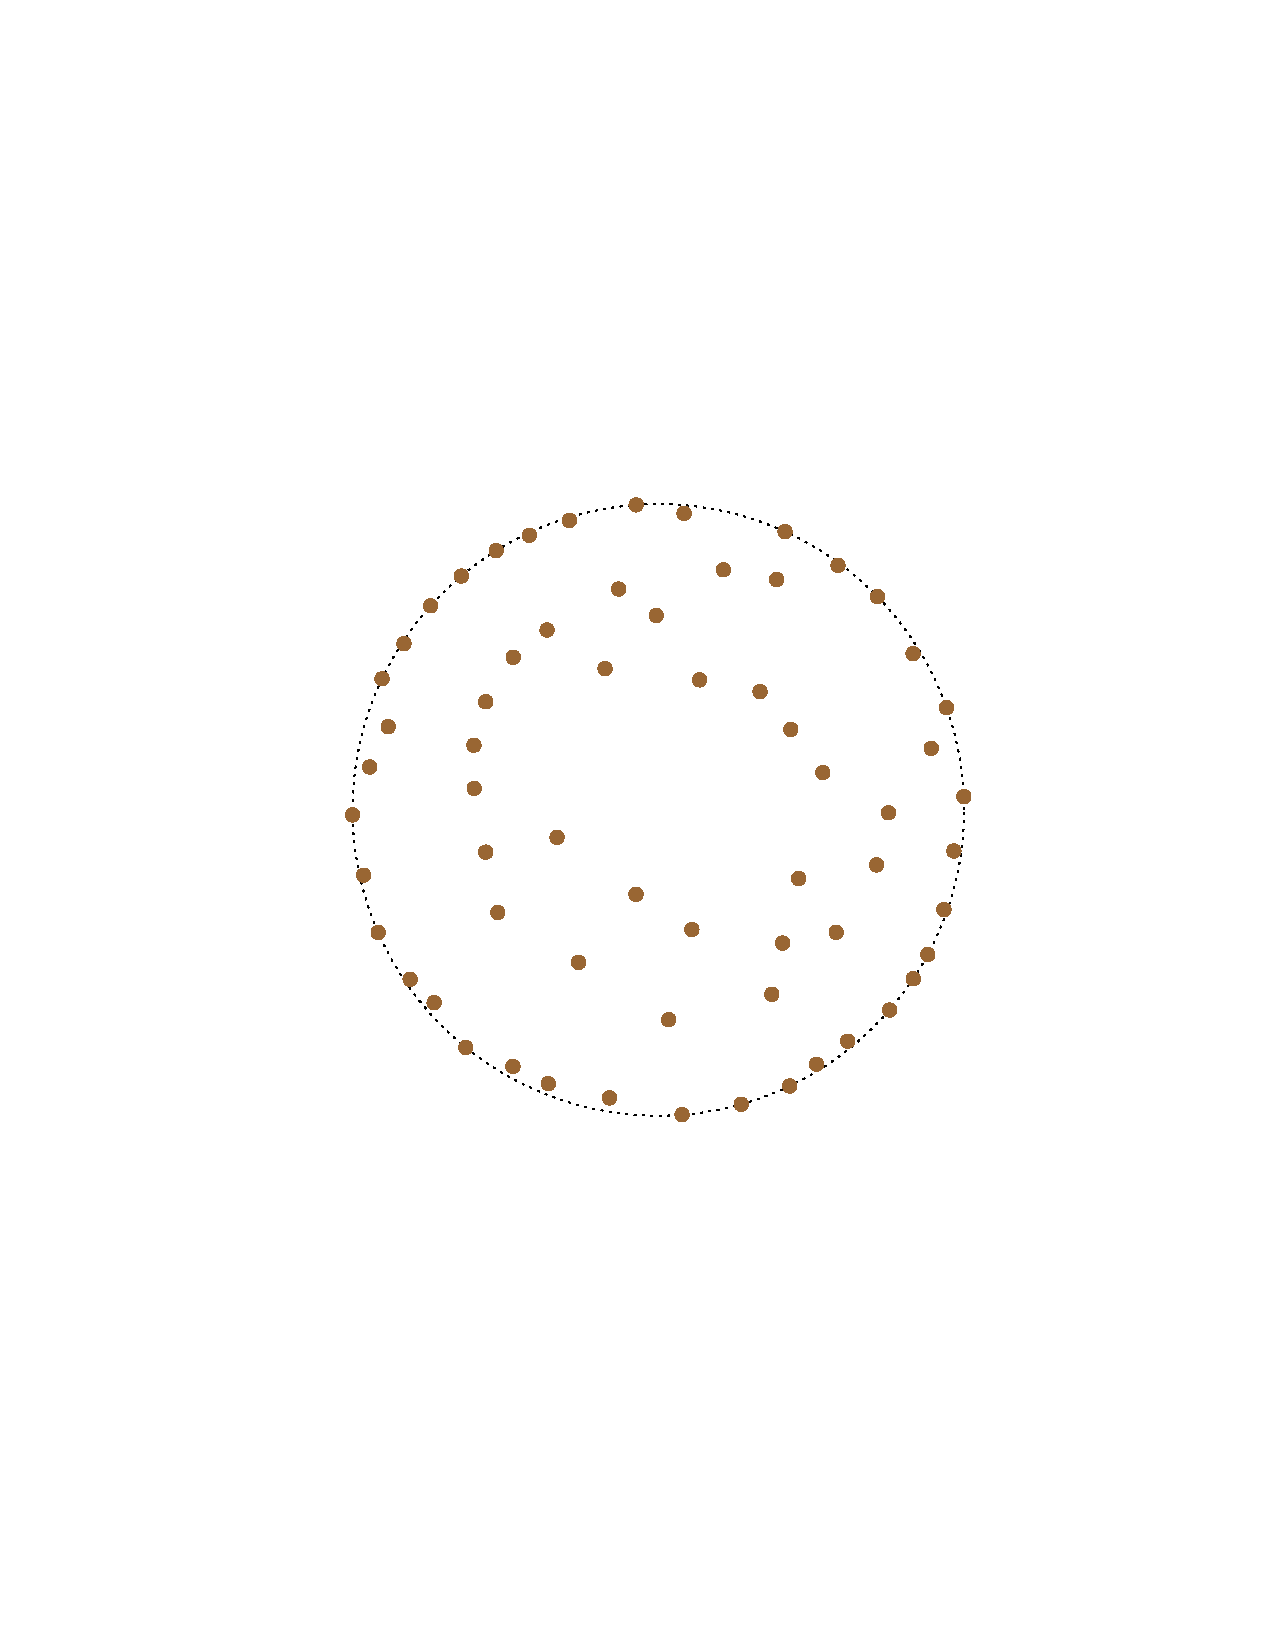
\includegraphics[clip, width=0.3\textwidth, scale=0.025, trim={3cm 8cm 3cm 8cm}]{figures/iea37-opt64-par11.pdf}
	}
	\subfigure[\textit{sub12}]{
		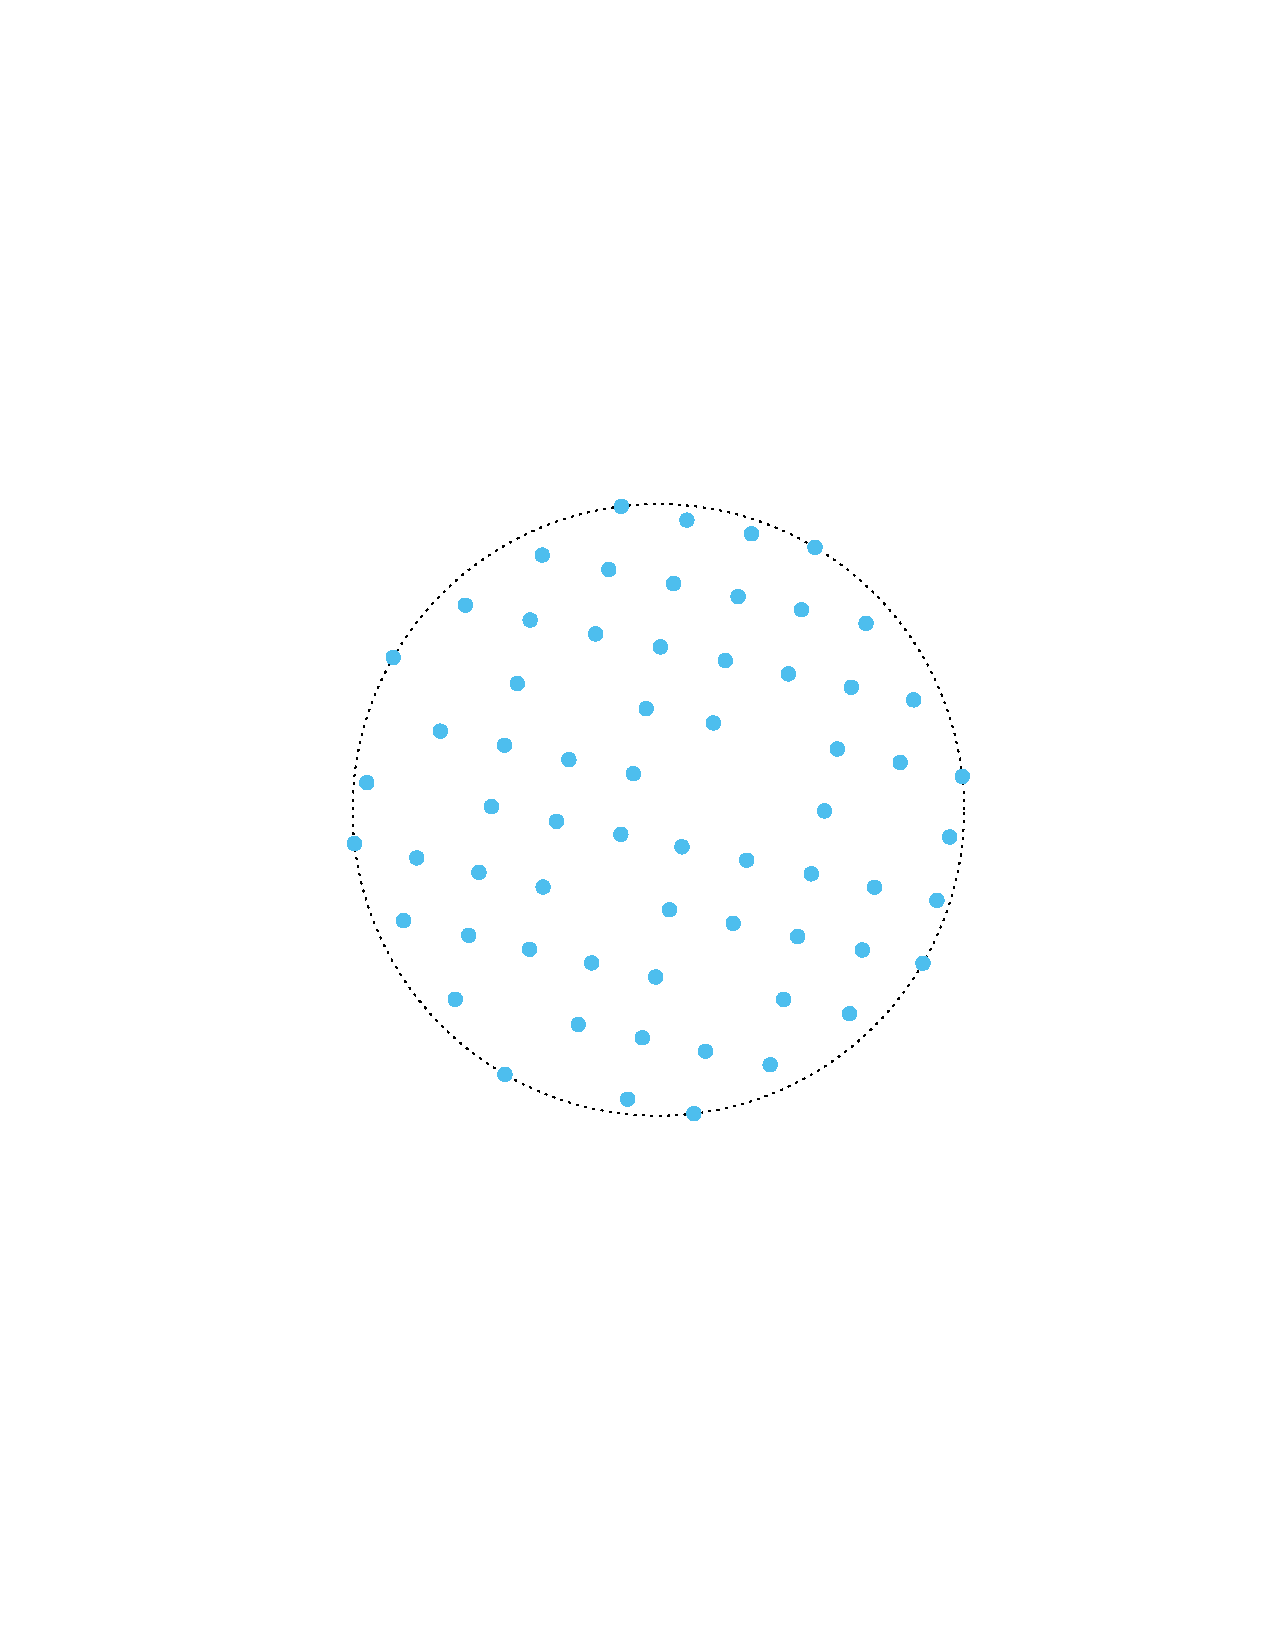
\includegraphics[clip, width=0.3\textwidth, scale=0.025, trim={3cm 8cm 3cm 8cm}]{figures/iea37-opt64-par12.pdf}
	}
	\caption{Case study 1: optimized wind farm layouts with 64 wind turbines.}
	
	\label{fig:64turbs}
\end{figure}

\end{document}